\documentclass[twoside]{book}

% Packages required by doxygen
\usepackage{fixltx2e}
\usepackage{calc}
\usepackage{doxygen}
\usepackage[export]{adjustbox} % also loads graphicx
\usepackage{graphicx}
\usepackage[utf8]{inputenc}
\usepackage{makeidx}
\usepackage{multicol}
\usepackage{multirow}
\PassOptionsToPackage{warn}{textcomp}
\usepackage{textcomp}
\usepackage[nointegrals]{wasysym}
\usepackage[table]{xcolor}

% Font selection
\usepackage[T1]{fontenc}
\usepackage[scaled=.90]{helvet}
\usepackage{courier}
\usepackage{amssymb}
\usepackage{sectsty}
\renewcommand{\familydefault}{\sfdefault}
\allsectionsfont{%
  \fontseries{bc}\selectfont%
  \color{darkgray}%
}
\renewcommand{\DoxyLabelFont}{%
  \fontseries{bc}\selectfont%
  \color{darkgray}%
}
\newcommand{\+}{\discretionary{\mbox{\scriptsize$\hookleftarrow$}}{}{}}

% Page & text layout
\usepackage{geometry}
\geometry{%
  a4paper,%
  top=2.5cm,%
  bottom=2.5cm,%
  left=2.5cm,%
  right=2.5cm%
}
\tolerance=750
\hfuzz=15pt
\hbadness=750
\setlength{\emergencystretch}{15pt}
\setlength{\parindent}{0cm}
\setlength{\parskip}{3ex plus 2ex minus 2ex}
\makeatletter
\renewcommand{\paragraph}{%
  \@startsection{paragraph}{4}{0ex}{-1.0ex}{1.0ex}{%
    \normalfont\normalsize\bfseries\SS@parafont%
  }%
}
\renewcommand{\subparagraph}{%
  \@startsection{subparagraph}{5}{0ex}{-1.0ex}{1.0ex}{%
    \normalfont\normalsize\bfseries\SS@subparafont%
  }%
}
\makeatother

% Headers & footers
\usepackage{fancyhdr}
\pagestyle{fancyplain}
\fancyhead[LE]{\fancyplain{}{\bfseries\thepage}}
\fancyhead[CE]{\fancyplain{}{}}
\fancyhead[RE]{\fancyplain{}{\bfseries\leftmark}}
\fancyhead[LO]{\fancyplain{}{\bfseries\rightmark}}
\fancyhead[CO]{\fancyplain{}{}}
\fancyhead[RO]{\fancyplain{}{\bfseries\thepage}}
\fancyfoot[LE]{\fancyplain{}{}}
\fancyfoot[CE]{\fancyplain{}{}}
\fancyfoot[RE]{\fancyplain{}{\bfseries\scriptsize Generated by Doxygen }}
\fancyfoot[LO]{\fancyplain{}{\bfseries\scriptsize Generated by Doxygen }}
\fancyfoot[CO]{\fancyplain{}{}}
\fancyfoot[RO]{\fancyplain{}{}}
\renewcommand{\footrulewidth}{0.4pt}
\renewcommand{\chaptermark}[1]{%
  \markboth{#1}{}%
}
\renewcommand{\sectionmark}[1]{%
  \markright{\thesection\ #1}%
}

% Indices & bibliography
\usepackage{natbib}
\usepackage[titles]{tocloft}
\setcounter{tocdepth}{3}
\setcounter{secnumdepth}{5}
\makeindex

% Hyperlinks (required, but should be loaded last)
\usepackage{ifpdf}
\ifpdf
  \usepackage[pdftex,pagebackref=true]{hyperref}
\else
  \usepackage[ps2pdf,pagebackref=true]{hyperref}
\fi
\hypersetup{%
  colorlinks=true,%
  linkcolor=blue,%
  citecolor=blue,%
  unicode%
}

% Custom commands
\newcommand{\clearemptydoublepage}{%
  \newpage{\pagestyle{empty}\cleardoublepage}%
}

\usepackage{caption}
\captionsetup{labelsep=space,justification=centering,font={bf},singlelinecheck=off,skip=4pt,position=top}

%===== C O N T E N T S =====

\begin{document}

% Titlepage & ToC
\hypersetup{pageanchor=false,
             bookmarksnumbered=true,
             pdfencoding=unicode
            }
\pagenumbering{roman}
\begin{titlepage}
\vspace*{7cm}
\begin{center}%
{\Large Multi-\/\+Robot-\/\+System }\\
\vspace*{1cm}
{\large Generated by Doxygen 1.8.11}\\
\end{center}
\end{titlepage}
\clearemptydoublepage
\tableofcontents
\clearemptydoublepage
\pagenumbering{arabic}
\hypersetup{pageanchor=true}

%--- Begin generated contents ---
\chapter{R\+E\+A\+D\+ME}
\label{md_gazebo_ros_link_attacher_README}
\hypertarget{md_gazebo_ros_link_attacher_README}{}
Attach two Gazebo models with a virtual joint in a generalized grasp hack

\section*{Build}


\begin{DoxyCode}
1 mkdir -p gazebo\_link\_attacher\_ws/src
2 cd gazebo\_link\_attacher\_ws/src
3 catkin\_init\_workspace
4 git clone https://github.com/pal-robotics/gazebo\_ros\_link\_attacher.git
5 cd ..
6 catkin\_make
7 source devel/setup.bash
\end{DoxyCode}


\section*{Launch}

\begin{DoxyVerb}roslaunch gazebo_ros_link_attacher test_attacher.launch
\end{DoxyVerb}


Empty world with the plugin {\ttfamily libgazebo\+\_\+ros\+\_\+link\+\_\+attacher.\+so} loaded (in the {\itshape worlds} folder).

Which provides the {\ttfamily /link\+\_\+attacher\+\_\+node/attach} service to specify two models and their links to be attached.

And {\ttfamily /link\+\_\+attacher\+\_\+node/detach} service to specify two models and their links to be detached.



\section*{Run demo}

In another shell, be sure to do {\ttfamily source devel/setup.\+bash} of your workspace. \begin{DoxyVerb}rosrun gazebo_ros_link_attacher spawn.py
\end{DoxyVerb}


Three cubes will be spawned. \begin{DoxyVerb}rosrun gazebo_ros_link_attacher attach.py
\end{DoxyVerb}


The cubes will be attached all between themselves as (1,2), (2,3), (3,1). You can move them with the G\+UI and you\textquotesingle{}ll see they will move together. \begin{DoxyVerb}rosrun gazebo_ros_link_attacher detach.py
\end{DoxyVerb}


The cubes will be detached and you can move them separately again.

You can also spawn items with the G\+UI and run a rosservice call\+: 
\begin{DoxyCode}
1 rosservice call /link\_attacher\_node/attach "model\_name\_1: 'unit\_box\_1'
2 link\_name\_1: 'link'
3 model\_name\_2: 'unit\_sphere\_1'
4 link\_name\_2: 'link'"
\end{DoxyCode}


And same thing to detach\+: 
\begin{DoxyCode}
1 rosservice call /link\_attacher\_node/detach "model\_name\_1: 'unit\_box\_1'
2 link\_name\_1: 'link'
3 model\_name\_2: 'unit\_sphere\_1'
4 link\_name\_2: 'link'"
\end{DoxyCode}


\section*{Current status}

It works!

$\sim$$\sim$\+Currently it crashes with\+:$\sim$$\sim$


\begin{DoxyCode}
1 ***** Internal Program Error - assertion (self->inertial != \_\_null) failed in static void
       gazebo::physics::ODELink::MoveCallback(dBodyID):
2 /tmp/buildd/gazebo4-4.1.3/gazebo/physics/ode/ODELink.cc(178): Inertial pointer is NULL
3 Aborted (core dumped)
\end{DoxyCode}


$\sim$$\sim$\+Which I\textquotesingle{}ve only seen this other useful information\+: \href{https://bitbucket.org/osrf/gazebo/issues/1177/removing-moving-model-with-ode-friction}{\tt Bitbucket gazebo removing moving model with ode friction fails}. But it didn\textquotesingle{}t help me solve my crash. I guess when attaching one model to the other it removes the second one to re-\/create it attached to the first or something like that.$\sim$$\sim$

$\sim$$\sim$\+And also this other issue\+: \href{https://bitbucket.org/osrf/gazebo/issues/1077/visualizing-dynamically-created-joints}{\tt Visualizing dynamically created joints} made me add a couple of lines more.$\sim$$\sim$

$\sim$$\sim$\+The method to attach the links is based on the grasp hack of the Gripper in gazebo/physics\+: \href{https://bitbucket.org/osrf/gazebo/src/1d1e3a542af81670f43a120e1df7190592bc4c0f/gazebo/physics/Gripper.hh?at=default&fileviewer=file-view-default}{\tt Gripper.\+hh} \href{https://bitbucket.org/osrf/gazebo/src/1d1e3a542af81670f43a120e1df7190592bc4c0f/gazebo/physics/Gripper.cc?at=default&fileviewer=file-view-default}{\tt Gripper.\+cc}$\sim$$\sim$

$\sim$$\sim$\+Which is to create a revolute joint on the first model (with range of motion 0) linking a link on the first model and a link on the second model.$\sim$$\sim$ 
\chapter{Definition of launchfiles\+:}
\label{md_README}
\hypertarget{md_README}{}
Launchfiles for launching the implemented functionalities are given in /multi\+\_\+robot\+\_\+launcher/launch
\begin{DoxyEnumerate}
\item exe\+\_\+demo.\+launch\+: Executes a demo environment within basic funcitonalities of the robot formation can be shown.
\item exe\+\_\+navigation.\+launch\+: Executes an environment within the robot formation can be used in combination with the navigation\+\_\+stack.
\item exe\+\_\+transport.\+launch\+: Executes an environment within the robot formation is carrying a transport object.
\item formation.\+launch\+: This is one of the most important launchfiles for using mobile robot formation. It launchs the robots for the formation and does the nescessary remaping for member parameters.
\item gazebo. launch\+: Just launches the gazeob environment.
\item robot.\+launch\+: This launches the hole robot stuff. Eg. The robot state publisher the localisation node for extended kalman filter and loads parameter for these modules. This file does N\+OT load the Foramtion controller since this is located within the controller package!
\item simulation.\+launch\+: Prepares simulations from skript files (see bash).
\item spawn\+\_\+transport\+\_\+object.\+launch A launch files that is used to spawn generic transport object
\end{DoxyEnumerate}

\section*{How to start a simple formation\+:}


\begin{DoxyEnumerate}
\item Execute exe\+\_\+demo.\+launch {\ttfamily \$roslaunch multi\+\_\+robot\+\_\+launcher exe\+\_\+demo.\+launch}
\item Wait til everything is setup
\item Execute the system handling node {\ttfamily \$rosrun simulation\+\_\+env system\+\_\+handling\+\_\+node -\/plan -\/reference}
\end{DoxyEnumerate}

\section*{How to modifie formation parameters\+:}


\begin{DoxyEnumerate}
\item Goto foramtion.\+yaml in the multi\+\_\+robot\+\_\+launcher package
\item Change the parameter within the file 2a) If you change the number or names of formation memebers make sure that you do the same in the formation.\+launch file in mutli\+\_\+robot\+\_\+launcher package 
\end{DoxyEnumerate}
\chapter{Hierarchical Index}
\section{Class Hierarchy}
This inheritance list is sorted roughly, but not completely, alphabetically\+:\begin{DoxyCompactList}
\item \contentsline{section}{Circle\+Planner\+:\+:Circle\+Plan}{\pageref{structCirclePlanner_1_1CirclePlan}}{}
\item \contentsline{section}{Controller}{\pageref{classController}}{}
\begin{DoxyCompactList}
\item \contentsline{section}{Master}{\pageref{classMaster}}{}
\item \contentsline{section}{Slave}{\pageref{classSlave}}{}
\end{DoxyCompactList}
\item \contentsline{section}{Controller\+:\+:Control\+State}{\pageref{structController_1_1ControlState}}{}
\item \contentsline{section}{Controller\+:\+:Control\+Vector}{\pageref{structController_1_1ControlVector}}{}
\item \contentsline{section}{Laser\+Predictor\+:\+:Data}{\pageref{structLaserPredictor_1_1Data}}{}
\item \contentsline{section}{Formation}{\pageref{classFormation}}{}
\item \contentsline{section}{Formation\+Publisher}{\pageref{classFormationPublisher}}{}
\item \contentsline{section}{Formation\+Subscriber}{\pageref{classFormationSubscriber}}{}
\item \contentsline{section}{Laser\+Predictor\+:\+:Frames}{\pageref{structLaserPredictor_1_1Frames}}{}
\item \contentsline{section}{Laser\+Predictor}{\pageref{classLaserPredictor}}{}
\item \contentsline{section}{Lissajous\+Planner\+:\+:Lissajous\+Plan}{\pageref{structLissajousPlanner_1_1LissajousPlan}}{}
\item \contentsline{section}{Controller\+:\+:Lyapunov\+Parameter}{\pageref{structController_1_1LyapunovParameter}}{}
\item \contentsline{section}{Planner}{\pageref{classPlanner}}{}
\begin{DoxyCompactList}
\item \contentsline{section}{Circle\+Planner}{\pageref{classCirclePlanner}}{}
\item \contentsline{section}{Clicked\+Pose\+Planner}{\pageref{classClickedPosePlanner}}{}
\item \contentsline{section}{Lissajous\+Planner}{\pageref{classLissajousPlanner}}{}
\item \contentsline{section}{Spiralplanner}{\pageref{classSpiralplanner}}{}
\end{DoxyCompactList}
\item \contentsline{section}{Spiralplanner\+:\+:Spiral\+Plan}{\pageref{structSpiralplanner_1_1SpiralPlan}}{}
\item \contentsline{section}{Laser\+Predictor\+:\+:Transforms}{\pageref{structLaserPredictor_1_1Transforms}}{}
\end{DoxyCompactList}

\chapter{Class Index}
\section{Class List}
Here are the classes, structs, unions and interfaces with brief descriptions\+:\begin{DoxyCompactList}
\item\contentsline{section}{\hyperlink{structController_1_1AngleDistanceParameter}{Controller\+::\+Angle\+Distance\+Parameter} \\*Specifies the Parameters of the angle distance based control law }{\pageref{d5/d97/structController_1_1AngleDistanceParameter}}{}
\item\contentsline{section}{\hyperlink{structController_1_1Buffer}{Controller\+::\+Buffer$<$ T $>$} \\*Template for a buffer of a given size and a given type }{\pageref{da/df9/structController_1_1Buffer}}{}
\item\contentsline{section}{\hyperlink{structCirclePlanner_1_1CirclePlan}{Circle\+Planner\+::\+Circle\+Plan} }{\pageref{dc/d44/structCirclePlanner_1_1CirclePlan}}{}
\item\contentsline{section}{\hyperlink{classCirclePlanner}{Circle\+Planner} }{\pageref{dc/d00/classCirclePlanner}}{}
\item\contentsline{section}{\hyperlink{classClickedPosePlanner}{Clicked\+Pose\+Planner} }{\pageref{dc/de5/classClickedPosePlanner}}{}
\item\contentsline{section}{\hyperlink{classController}{Controller} \\*Provides a easy to use implementation of a generic mobile robot controller }{\pageref{d9/d85/classController}}{}
\item\contentsline{section}{\hyperlink{structController_1_1ControlState}{Controller\+::\+Control\+State} \\*Holds the System state combined by the pose of the system, the cartesian velocity and the angular velocity }{\pageref{df/d22/structController_1_1ControlState}}{}
\item\contentsline{section}{\hyperlink{structController_1_1ControlVector}{Controller\+::\+Control\+Vector} \\*A struct that holds linear and angular velocity of the Robot since this are the control variable for kinematic tracking control }{\pageref{da/ddc/structController_1_1ControlVector}}{}
\item\contentsline{section}{\hyperlink{structLaserPredictor_1_1Data}{Laser\+Predictor\+::\+Data} \\*Holds all the data used within the predictor }{\pageref{de/d78/structLaserPredictor_1_1Data}}{}
\item\contentsline{section}{\hyperlink{structgazebo_1_1GazeboRosLinkAttacher_1_1fixedJoint}{gazebo\+::\+Gazebo\+Ros\+Link\+Attacher\+::fixed\+Joint} \\*Internal representation of a fixed joint }{\pageref{d8/d07/structgazebo_1_1GazeboRosLinkAttacher_1_1fixedJoint}}{}
\item\contentsline{section}{\hyperlink{classFormation}{Formation} \\*A Class for handeling basic mobile \hyperlink{structFormation_1_1Robot}{Robot} formation work. Properly adds Robots to a formation and provides basic interpretation tools as the adjacency matrix of the formation }{\pageref{d0/d39/classFormation}}{}
\item\contentsline{section}{\hyperlink{classFormationPublisher}{Formation\+Publisher} }{\pageref{d1/da9/classFormationPublisher}}{}
\item\contentsline{section}{\hyperlink{classFormationSubscriber}{Formation\+Subscriber} }{\pageref{d8/dc8/classFormationSubscriber}}{}
\item\contentsline{section}{\hyperlink{structLaserPredictor_1_1Frames}{Laser\+Predictor\+::\+Frames} \\*Holds the names of all the necessary frames for the prediction class }{\pageref{d1/d8b/structLaserPredictor_1_1Frames}}{}
\item\contentsline{section}{\hyperlink{classgazebo_1_1GazeboRosLinkAttacher}{gazebo\+::\+Gazebo\+Ros\+Link\+Attacher} }{\pageref{dd/d29/classgazebo_1_1GazeboRosLinkAttacher}}{}
\item\contentsline{section}{\hyperlink{classLaserPredictor}{Laser\+Predictor} \\*A class for predictings neighbour robots from the laser scanner data of another robot }{\pageref{d1/dc0/classLaserPredictor}}{}
\item\contentsline{section}{\hyperlink{structLissajousPlanner_1_1LissajousPlan}{Lissajous\+Planner\+::\+Lissajous\+Plan} }{\pageref{d1/d0f/structLissajousPlanner_1_1LissajousPlan}}{}
\item\contentsline{section}{\hyperlink{classLissajousPlanner}{Lissajous\+Planner} }{\pageref{d5/dbf/classLissajousPlanner}}{}
\item\contentsline{section}{\hyperlink{structController_1_1LyapunovParameter}{Controller\+::\+Lyapunov\+Parameter} \\*Specifies the parameters needed for the lyapunov based control law }{\pageref{da/d3d/structController_1_1LyapunovParameter}}{}
\item\contentsline{section}{\hyperlink{classMaster}{Master} \\*Class that implements a master robot for multi robot formation control }{\pageref{d2/dbd/classMaster}}{}
\item\contentsline{section}{\hyperlink{classOdometryPredictor}{Odometry\+Predictor} }{\pageref{d6/d6d/classOdometryPredictor}}{}
\item\contentsline{section}{\hyperlink{classPlanner}{Planner} \\*A generic planner class that provides general interface functions and architecture }{\pageref{da/dfa/classPlanner}}{}
\item\contentsline{section}{\hyperlink{structFormation_1_1Robot}{Formation\+::\+Robot} \\*Holds a robot to handle with formation member stuff }{\pageref{d0/da7/structFormation_1_1Robot}}{}
\item\contentsline{section}{\hyperlink{structFormation_1_1RobotProperties}{Formation\+::\+Robot\+Properties} \\*Defines Properties of a \hyperlink{structFormation_1_1Robot}{Robot} }{\pageref{d3/d81/structFormation_1_1RobotProperties}}{}
\item\contentsline{section}{\hyperlink{classSlave}{Slave} \\*Class that implements a slave robot for multi robot formation control }{\pageref{d8/d18/classSlave}}{}
\item\contentsline{section}{\hyperlink{structSpiralplanner_1_1SpiralPlan}{Spiralplanner\+::\+Spiral\+Plan} }{\pageref{d2/dd8/structSpiralplanner_1_1SpiralPlan}}{}
\item\contentsline{section}{\hyperlink{classSpiralplanner}{Spiralplanner} }{\pageref{d4/dd5/classSpiralplanner}}{}
\item\contentsline{section}{\hyperlink{structStepResposePlanner_1_1StepPlan}{Step\+Respose\+Planner\+::\+Step\+Plan} }{\pageref{d5/d69/structStepResposePlanner_1_1StepPlan}}{}
\item\contentsline{section}{\hyperlink{classStepResposePlanner}{Step\+Respose\+Planner} }{\pageref{d6/d2a/classStepResposePlanner}}{}
\item\contentsline{section}{\hyperlink{structLaserPredictor_1_1Transforms}{Laser\+Predictor\+::\+Transforms} \\*Holds all necessary transformations }{\pageref{d6/d09/structLaserPredictor_1_1Transforms}}{}
\end{DoxyCompactList}

\chapter{Class Documentation}
\hypertarget{structController_1_1AngleDistanceParameter}{}\section{Controller\+:\+:Angle\+Distance\+Parameter Struct Reference}
\label{structController_1_1AngleDistanceParameter}\index{Controller\+::\+Angle\+Distance\+Parameter@{Controller\+::\+Angle\+Distance\+Parameter}}


Specifies the Parameters of the angle distance based control law.  




{\ttfamily \#include $<$controller.\+h$>$}

\subsection*{Public Member Functions}
\begin{DoxyCompactItemize}
\item 
\hyperlink{structController_1_1AngleDistanceParameter_a13a71741708edb6c837fe7ff40840dde}{Angle\+Distance\+Parameter} ()\hypertarget{structController_1_1AngleDistanceParameter_a13a71741708edb6c837fe7ff40840dde}{}\label{structController_1_1AngleDistanceParameter_a13a71741708edb6c837fe7ff40840dde}

\begin{DoxyCompactList}\small\item\em Construct a new Angle Distance Parameter object, with default parameters. \end{DoxyCompactList}\item 
\hyperlink{structController_1_1AngleDistanceParameter_a07d302639f766797f8dd427935c882c2}{Angle\+Distance\+Parameter} (float \hyperlink{structController_1_1AngleDistanceParameter_ac2bab50d5c5f357d05632e3abc463dbf}{angular\+\_\+gain}, float \hyperlink{structController_1_1AngleDistanceParameter_a519dfcbf82e3e44a9a315b91964fa7de}{linear\+\_\+gain}, float \hyperlink{structController_1_1AngleDistanceParameter_a360e632b14647dce7dbadf168901880c}{d})
\begin{DoxyCompactList}\small\item\em Construct a new Angle Distance Parameter with given parameters. \end{DoxyCompactList}\item 
\hyperlink{structController_1_1AngleDistanceParameter_ab77c9431c35886760e7a2fb659008ab2}{Angle\+Distance\+Parameter} (std\+::vector$<$ float $>$ param)
\begin{DoxyCompactList}\small\item\em Construct a new Angle Distance Parameter from a given vector of parameters. \end{DoxyCompactList}\end{DoxyCompactItemize}
\subsection*{Public Attributes}
\begin{DoxyCompactItemize}
\item 
float \hyperlink{structController_1_1AngleDistanceParameter_ac2bab50d5c5f357d05632e3abc463dbf}{angular\+\_\+gain}\hypertarget{structController_1_1AngleDistanceParameter_ac2bab50d5c5f357d05632e3abc463dbf}{}\label{structController_1_1AngleDistanceParameter_ac2bab50d5c5f357d05632e3abc463dbf}

\begin{DoxyCompactList}\small\item\em Control gain in phi direction. \end{DoxyCompactList}\item 
float \hyperlink{structController_1_1AngleDistanceParameter_a519dfcbf82e3e44a9a315b91964fa7de}{linear\+\_\+gain}\hypertarget{structController_1_1AngleDistanceParameter_a519dfcbf82e3e44a9a315b91964fa7de}{}\label{structController_1_1AngleDistanceParameter_a519dfcbf82e3e44a9a315b91964fa7de}

\begin{DoxyCompactList}\small\item\em Control gain in l direction. \end{DoxyCompactList}\item 
float \hyperlink{structController_1_1AngleDistanceParameter_a360e632b14647dce7dbadf168901880c}{d}\hypertarget{structController_1_1AngleDistanceParameter_a360e632b14647dce7dbadf168901880c}{}\label{structController_1_1AngleDistanceParameter_a360e632b14647dce7dbadf168901880c}

\begin{DoxyCompactList}\small\item\em parameter for collision avoidance \end{DoxyCompactList}\end{DoxyCompactItemize}


\subsection{Detailed Description}
Specifies the Parameters of the angle distance based control law. 

\subsection{Constructor \& Destructor Documentation}
\index{Controller\+::\+Angle\+Distance\+Parameter@{Controller\+::\+Angle\+Distance\+Parameter}!Angle\+Distance\+Parameter@{Angle\+Distance\+Parameter}}
\index{Angle\+Distance\+Parameter@{Angle\+Distance\+Parameter}!Controller\+::\+Angle\+Distance\+Parameter@{Controller\+::\+Angle\+Distance\+Parameter}}
\subsubsection[{\texorpdfstring{Angle\+Distance\+Parameter(float angular\+\_\+gain, float linear\+\_\+gain, float d)}{AngleDistanceParameter(float angular_gain, float linear_gain, float d)}}]{\setlength{\rightskip}{0pt plus 5cm}Controller\+::\+Angle\+Distance\+Parameter\+::\+Angle\+Distance\+Parameter (
\begin{DoxyParamCaption}
\item[{float}]{angular\+\_\+gain, }
\item[{float}]{linear\+\_\+gain, }
\item[{float}]{d}
\end{DoxyParamCaption}
)\hspace{0.3cm}{\ttfamily [inline]}}\hypertarget{structController_1_1AngleDistanceParameter_a07d302639f766797f8dd427935c882c2}{}\label{structController_1_1AngleDistanceParameter_a07d302639f766797f8dd427935c882c2}


Construct a new Angle Distance Parameter with given parameters. 


\begin{DoxyParams}{Parameters}
{\em angular\+\_\+gain} & ///$<$Gain in Angular direction (phi/psi direction) \\
\hline
{\em linear\+\_\+gain} & ///$<$Gain in linear direction (distance direction) \\
\hline
{\em d} & ///$<$Collision avoidance paramtere \\
\hline
\end{DoxyParams}
\index{Controller\+::\+Angle\+Distance\+Parameter@{Controller\+::\+Angle\+Distance\+Parameter}!Angle\+Distance\+Parameter@{Angle\+Distance\+Parameter}}
\index{Angle\+Distance\+Parameter@{Angle\+Distance\+Parameter}!Controller\+::\+Angle\+Distance\+Parameter@{Controller\+::\+Angle\+Distance\+Parameter}}
\subsubsection[{\texorpdfstring{Angle\+Distance\+Parameter(std\+::vector$<$ float $>$ param)}{AngleDistanceParameter(std::vector< float > param)}}]{\setlength{\rightskip}{0pt plus 5cm}Controller\+::\+Angle\+Distance\+Parameter\+::\+Angle\+Distance\+Parameter (
\begin{DoxyParamCaption}
\item[{std\+::vector$<$ float $>$}]{param}
\end{DoxyParamCaption}
)\hspace{0.3cm}{\ttfamily [inline]}}\hypertarget{structController_1_1AngleDistanceParameter_ab77c9431c35886760e7a2fb659008ab2}{}\label{structController_1_1AngleDistanceParameter_ab77c9431c35886760e7a2fb659008ab2}


Construct a new Angle Distance Parameter from a given vector of parameters. 


\begin{DoxyParams}{Parameters}
{\em param} & vector that must contain the three parameters of the object \\
\hline
\end{DoxyParams}


The documentation for this struct was generated from the following file\+:\begin{DoxyCompactItemize}
\item 
controller/include/controller/controller.\+h\end{DoxyCompactItemize}

\hypertarget{structController_1_1Buffer}{}\section{Controller\+:\+:Buffer$<$ T $>$ Struct Template Reference}
\label{structController_1_1Buffer}\index{Controller\+::\+Buffer$<$ T $>$@{Controller\+::\+Buffer$<$ T $>$}}


Template for a buffer of a given size and a given type.  




{\ttfamily \#include $<$controller.\+h$>$}

\subsection*{Public Member Functions}
\begin{DoxyCompactItemize}
\item 
\hyperlink{structController_1_1Buffer_af9a6e1eefa379cbbaac009f7ee3e6912}{Buffer} ()\hypertarget{structController_1_1Buffer_af9a6e1eefa379cbbaac009f7ee3e6912}{}\label{structController_1_1Buffer_af9a6e1eefa379cbbaac009f7ee3e6912}

\begin{DoxyCompactList}\small\item\em Construct a new \hyperlink{structController_1_1Buffer}{Buffer} object with default size. \end{DoxyCompactList}\item 
\hyperlink{structController_1_1Buffer_a05279a3252b1896a35459387458abd4b}{Buffer} (int size)
\begin{DoxyCompactList}\small\item\em Construct a new \hyperlink{structController_1_1Buffer}{Buffer} object of given size. \end{DoxyCompactList}\item 
void \hyperlink{structController_1_1Buffer_aeb29555b9b1be00916e2a631128f103c}{insert} (T element)
\begin{DoxyCompactList}\small\item\em Insert an element into the buffer. \end{DoxyCompactList}\item 
std\+::vector$<$ T $>$ \hyperlink{structController_1_1Buffer_a6b5ebe18f4fff2824f3797c8afa3aced}{get} ()
\begin{DoxyCompactList}\small\item\em Get all currently buffered values. \end{DoxyCompactList}\end{DoxyCompactItemize}
\subsection*{Public Attributes}
\begin{DoxyCompactItemize}
\item 
int \hyperlink{structController_1_1Buffer_a51dd1dc69f114ea7d8585b8f57c3afe1}{size\+\_\+}\hypertarget{structController_1_1Buffer_a51dd1dc69f114ea7d8585b8f57c3afe1}{}\label{structController_1_1Buffer_a51dd1dc69f114ea7d8585b8f57c3afe1}

\begin{DoxyCompactList}\small\item\em Size of the buffer. \end{DoxyCompactList}\item 
int \hyperlink{structController_1_1Buffer_a66c08bfde369f73ce78e85967bd25e6a}{counter\+\_\+}\hypertarget{structController_1_1Buffer_a66c08bfde369f73ce78e85967bd25e6a}{}\label{structController_1_1Buffer_a66c08bfde369f73ce78e85967bd25e6a}

\begin{DoxyCompactList}\small\item\em Current insert index. \end{DoxyCompactList}\item 
std\+::vector$<$ T $>$ \hyperlink{structController_1_1Buffer_aea2f98d896048118af7014893198ddd6}{buffer\+\_\+}\hypertarget{structController_1_1Buffer_aea2f98d896048118af7014893198ddd6}{}\label{structController_1_1Buffer_aea2f98d896048118af7014893198ddd6}

\begin{DoxyCompactList}\small\item\em Buffered values. \end{DoxyCompactList}\end{DoxyCompactItemize}


\subsection{Detailed Description}
\subsubsection*{template$<$typename T$>$\\*
struct Controller\+::\+Buffer$<$ T $>$}

Template for a buffer of a given size and a given type. 


\begin{DoxyTemplParams}{Template Parameters}
{\em T} & type if the values to be buffered \\
\hline
\end{DoxyTemplParams}


\subsection{Constructor \& Destructor Documentation}
\index{Controller\+::\+Buffer@{Controller\+::\+Buffer}!Buffer@{Buffer}}
\index{Buffer@{Buffer}!Controller\+::\+Buffer@{Controller\+::\+Buffer}}
\subsubsection[{\texorpdfstring{Buffer(int size)}{Buffer(int size)}}]{\setlength{\rightskip}{0pt plus 5cm}template$<$typename T$>$ {\bf Controller\+::\+Buffer}$<$ T $>$\+::{\bf Buffer} (
\begin{DoxyParamCaption}
\item[{int}]{size}
\end{DoxyParamCaption}
)\hspace{0.3cm}{\ttfamily [inline]}}\hypertarget{structController_1_1Buffer_a05279a3252b1896a35459387458abd4b}{}\label{structController_1_1Buffer_a05279a3252b1896a35459387458abd4b}


Construct a new \hyperlink{structController_1_1Buffer}{Buffer} object of given size. 


\begin{DoxyParams}{Parameters}
{\em size} & size of the buffer (number of values to be buffered) \\
\hline
\end{DoxyParams}


\subsection{Member Function Documentation}
\index{Controller\+::\+Buffer@{Controller\+::\+Buffer}!get@{get}}
\index{get@{get}!Controller\+::\+Buffer@{Controller\+::\+Buffer}}
\subsubsection[{\texorpdfstring{get()}{get()}}]{\setlength{\rightskip}{0pt plus 5cm}template$<$typename T$>$ std\+::vector$<$T$>$ {\bf Controller\+::\+Buffer}$<$ T $>$\+::get (
\begin{DoxyParamCaption}
{}
\end{DoxyParamCaption}
)\hspace{0.3cm}{\ttfamily [inline]}}\hypertarget{structController_1_1Buffer_a6b5ebe18f4fff2824f3797c8afa3aced}{}\label{structController_1_1Buffer_a6b5ebe18f4fff2824f3797c8afa3aced}


Get all currently buffered values. 

\begin{DoxyReturn}{Returns}
std\+::vector$<$\+T$>$ vector of values within the buffer 
\end{DoxyReturn}
\index{Controller\+::\+Buffer@{Controller\+::\+Buffer}!insert@{insert}}
\index{insert@{insert}!Controller\+::\+Buffer@{Controller\+::\+Buffer}}
\subsubsection[{\texorpdfstring{insert(\+T element)}{insert(T element)}}]{\setlength{\rightskip}{0pt plus 5cm}template$<$typename T$>$ void {\bf Controller\+::\+Buffer}$<$ T $>$\+::insert (
\begin{DoxyParamCaption}
\item[{T}]{element}
\end{DoxyParamCaption}
)\hspace{0.3cm}{\ttfamily [inline]}}\hypertarget{structController_1_1Buffer_aeb29555b9b1be00916e2a631128f103c}{}\label{structController_1_1Buffer_aeb29555b9b1be00916e2a631128f103c}


Insert an element into the buffer. 


\begin{DoxyParams}{Parameters}
{\em element} & Element of type T to be buffered \\
\hline
\end{DoxyParams}


The documentation for this struct was generated from the following file\+:\begin{DoxyCompactItemize}
\item 
controller/include/controller/controller.\+h\end{DoxyCompactItemize}

\hypertarget{structCirclePlanner_1_1CirclePlan}{}\section{Circle\+Planner\+:\+:Circle\+Plan Struct Reference}
\label{structCirclePlanner_1_1CirclePlan}\index{Circle\+Planner\+::\+Circle\+Plan@{Circle\+Planner\+::\+Circle\+Plan}}
\subsection*{Public Attributes}
\begin{DoxyCompactItemize}
\item 
float {\bfseries r}\hypertarget{structCirclePlanner_1_1CirclePlan_a713b4aad1fdffcdc82cc2242a87c9203}{}\label{structCirclePlanner_1_1CirclePlan_a713b4aad1fdffcdc82cc2242a87c9203}

\item 
float {\bfseries omega}\hypertarget{structCirclePlanner_1_1CirclePlan_a3bd3fe64ecc478997f8ffe85be6aaa4e}{}\label{structCirclePlanner_1_1CirclePlan_a3bd3fe64ecc478997f8ffe85be6aaa4e}

\end{DoxyCompactItemize}


The documentation for this struct was generated from the following file\+:\begin{DoxyCompactItemize}
\item 
simulation\+\_\+env/include/simulation\+\_\+env/planner.\+h\end{DoxyCompactItemize}

\hypertarget{classCirclePlanner}{}\section{Circle\+Planner Class Reference}
\label{classCirclePlanner}\index{Circle\+Planner@{Circle\+Planner}}


Inheritance diagram for Circle\+Planner\+:\nopagebreak
\begin{figure}[H]
\begin{center}
\leavevmode
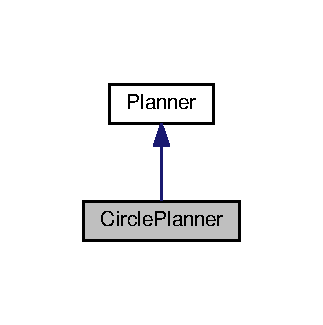
\includegraphics[width=155pt]{classCirclePlanner__inherit__graph}
\end{center}
\end{figure}


Collaboration diagram for Circle\+Planner\+:\nopagebreak
\begin{figure}[H]
\begin{center}
\leavevmode
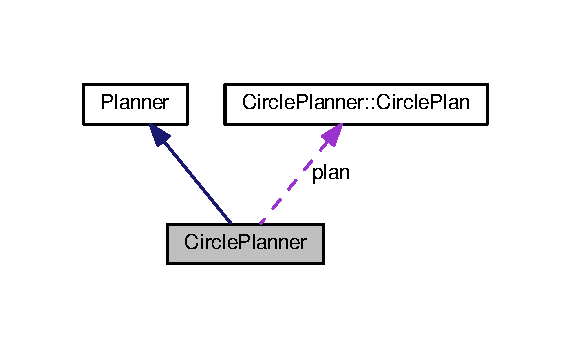
\includegraphics[width=274pt]{classCirclePlanner__coll__graph}
\end{center}
\end{figure}
\subsection*{Classes}
\begin{DoxyCompactItemize}
\item 
struct \hyperlink{structCirclePlanner_1_1CirclePlan}{Circle\+Plan}
\end{DoxyCompactItemize}
\subsection*{Public Member Functions}
\begin{DoxyCompactItemize}
\item 
{\bfseries Circle\+Planner} (ros\+::\+Node\+Handle \&\hyperlink{classPlanner_a9714d036f444a07ce90be8d135b9a40c}{nh})\hypertarget{classCirclePlanner_a33a27f97f5a1300d43c80b519fdfb3ef}{}\label{classCirclePlanner_a33a27f97f5a1300d43c80b519fdfb3ef}

\item 
void {\bfseries set\+\_\+parameter} (double r=3.\+0, double omega=0.\+5)\hypertarget{classCirclePlanner_a21fef783d5f2252fd1b53d93e869fc65}{}\label{classCirclePlanner_a21fef783d5f2252fd1b53d93e869fc65}

\item 
void {\bfseries load} ()\hypertarget{classCirclePlanner_a1c14f6ed36cbd32d39d60ed312a65de8}{}\label{classCirclePlanner_a1c14f6ed36cbd32d39d60ed312a65de8}

\end{DoxyCompactItemize}
\subsection*{Private Member Functions}
\begin{DoxyCompactItemize}
\item 
tf\+::\+Vector3 {\bfseries get\+\_\+position} (ros\+::\+Duration time)\hypertarget{classCirclePlanner_a1d6cdbec03a259af77937f0274dde5d9}{}\label{classCirclePlanner_a1d6cdbec03a259af77937f0274dde5d9}

\item 
tf\+::\+Quaternion {\bfseries get\+\_\+orientation} (ros\+::\+Duration time)\hypertarget{classCirclePlanner_a4e774b6cbc87a3dfa718df5594a0adbf}{}\label{classCirclePlanner_a4e774b6cbc87a3dfa718df5594a0adbf}

\item 
tf\+::\+Vector3 {\bfseries get\+\_\+velocity} (ros\+::\+Duration time)\hypertarget{classCirclePlanner_a5184277b2e174515140514fdec37ba29}{}\label{classCirclePlanner_a5184277b2e174515140514fdec37ba29}

\item 
double {\bfseries get\+\_\+angular\+\_\+velocity} (ros\+::\+Duration time)\hypertarget{classCirclePlanner_afa7c8502da92a63c78711ca92e73fe2b}{}\label{classCirclePlanner_afa7c8502da92a63c78711ca92e73fe2b}

\item 
void {\bfseries check\+\_\+period} (ros\+::\+Duration time)\hypertarget{classCirclePlanner_ab981788d76132e3f03ebedeb128d703a}{}\label{classCirclePlanner_ab981788d76132e3f03ebedeb128d703a}

\end{DoxyCompactItemize}
\subsection*{Private Attributes}
\begin{DoxyCompactItemize}
\item 
\hyperlink{structCirclePlanner_1_1CirclePlan}{Circle\+Plan} {\bfseries plan}\hypertarget{classCirclePlanner_a69f9e183351ef2c5325eef292350fb52}{}\label{classCirclePlanner_a69f9e183351ef2c5325eef292350fb52}

\end{DoxyCompactItemize}
\subsection*{Additional Inherited Members}


The documentation for this class was generated from the following files\+:\begin{DoxyCompactItemize}
\item 
simulation\+\_\+env/include/simulation\+\_\+env/planner.\+h\item 
simulation\+\_\+env/src/planner.\+cpp\end{DoxyCompactItemize}

\hypertarget{classClickedPosePlanner}{}\section{Clicked\+Pose\+Planner Class Reference}
\label{classClickedPosePlanner}\index{Clicked\+Pose\+Planner@{Clicked\+Pose\+Planner}}


Inheritance diagram for Clicked\+Pose\+Planner\+:\nopagebreak
\begin{figure}[H]
\begin{center}
\leavevmode
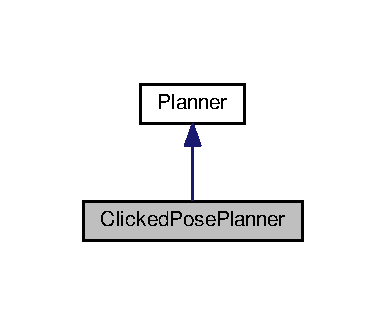
\includegraphics[width=185pt]{classClickedPosePlanner__inherit__graph}
\end{center}
\end{figure}


Collaboration diagram for Clicked\+Pose\+Planner\+:\nopagebreak
\begin{figure}[H]
\begin{center}
\leavevmode
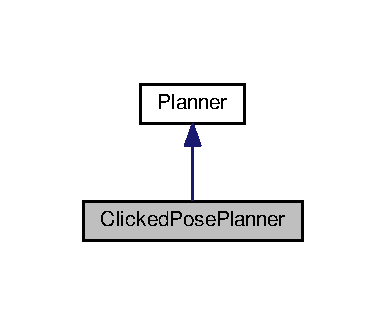
\includegraphics[width=185pt]{classClickedPosePlanner__coll__graph}
\end{center}
\end{figure}
\subsection*{Public Member Functions}
\begin{DoxyCompactItemize}
\item 
{\bfseries Clicked\+Pose\+Planner} (ros\+::\+Node\+Handle \&\hyperlink{classPlanner_a9714d036f444a07ce90be8d135b9a40c}{nh}, std\+::string topic\+\_\+name)\hypertarget{classClickedPosePlanner_a74a3e5f887074f15a88c617c5269ff6f}{}\label{classClickedPosePlanner_a74a3e5f887074f15a88c617c5269ff6f}

\item 
tf\+::\+Vector3 {\bfseries get\+\_\+position} (ros\+::\+Duration time)\hypertarget{classClickedPosePlanner_afc1871c54217d03e9e324f01b6f237a0}{}\label{classClickedPosePlanner_afc1871c54217d03e9e324f01b6f237a0}

\item 
tf\+::\+Quaternion {\bfseries get\+\_\+orientation} (ros\+::\+Duration time)\hypertarget{classClickedPosePlanner_ad0dc3f1824a1e8127cdda0d933700dec}{}\label{classClickedPosePlanner_ad0dc3f1824a1e8127cdda0d933700dec}

\item 
tf\+::\+Vector3 {\bfseries get\+\_\+velocity} (ros\+::\+Duration time)\hypertarget{classClickedPosePlanner_acdbdcf7b2e811542ccd812b72534bcfb}{}\label{classClickedPosePlanner_acdbdcf7b2e811542ccd812b72534bcfb}

\item 
tf\+::\+Vector3 {\bfseries get\+\_\+acceleration} (ros\+::\+Duration time)\hypertarget{classClickedPosePlanner_ade095ec782bd78a10dc397d039c49df1}{}\label{classClickedPosePlanner_ade095ec782bd78a10dc397d039c49df1}

\item 
double {\bfseries get\+\_\+angular\+\_\+velocity} (ros\+::\+Duration time)\hypertarget{classClickedPosePlanner_a29ea1f54b9103ffcffb13867c654c550}{}\label{classClickedPosePlanner_a29ea1f54b9103ffcffb13867c654c550}

\item 
void {\bfseries check\+\_\+period} (ros\+::\+Duration time)\hypertarget{classClickedPosePlanner_afa168a05970471ef34bd5ba19bbe4a0b}{}\label{classClickedPosePlanner_afa168a05970471ef34bd5ba19bbe4a0b}

\end{DoxyCompactItemize}
\subsection*{Private Member Functions}
\begin{DoxyCompactItemize}
\item 
void {\bfseries clicked\+Callback} (const geometry\+\_\+msgs\+::\+Pose\+Stamped\+Const\+Ptr msg)\hypertarget{classClickedPosePlanner_a14fd60114064f69a3d4569b10ce244d2}{}\label{classClickedPosePlanner_a14fd60114064f69a3d4569b10ce244d2}

\item 
void {\bfseries load\+Child} ()\hypertarget{classClickedPosePlanner_a8e8e18e8dc6e007bbd0ac40d5aba6076}{}\label{classClickedPosePlanner_a8e8e18e8dc6e007bbd0ac40d5aba6076}

\end{DoxyCompactItemize}
\subsection*{Private Attributes}
\begin{DoxyCompactItemize}
\item 
ros\+::\+Subscriber {\bfseries sub\+\_\+}\hypertarget{classClickedPosePlanner_ae9909d554dfd56cdf729bc9dfa24565b}{}\label{classClickedPosePlanner_ae9909d554dfd56cdf729bc9dfa24565b}

\item 
tf\+::\+Pose {\bfseries pose\+\_\+}\hypertarget{classClickedPosePlanner_a0edb2f1c085b602791a08a1528fe3c27}{}\label{classClickedPosePlanner_a0edb2f1c085b602791a08a1528fe3c27}

\item 
tf\+::\+Vector3 {\bfseries direction\+\_\+}\hypertarget{classClickedPosePlanner_aa677a316251a6a88adcaa52b3c71ea4b}{}\label{classClickedPosePlanner_aa677a316251a6a88adcaa52b3c71ea4b}

\end{DoxyCompactItemize}
\subsection*{Additional Inherited Members}


The documentation for this class was generated from the following files\+:\begin{DoxyCompactItemize}
\item 
simulation\+\_\+env/include/simulation\+\_\+env/planner.\+h\item 
simulation\+\_\+env/src/planner.\+cpp\end{DoxyCompactItemize}

\hypertarget{classController}{}\section{Controller Class Reference}
\label{classController}\index{Controller@{Controller}}


Provides a easy to use implementation of a generic mobile robot controller.  




{\ttfamily \#include $<$controller.\+h$>$}



Inheritance diagram for Controller\+:
\nopagebreak
\begin{figure}[H]
\begin{center}
\leavevmode
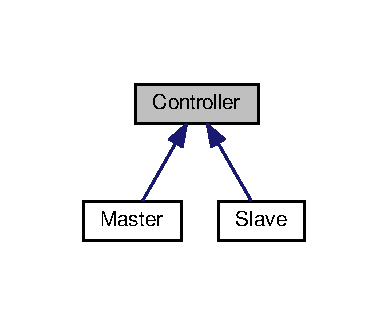
\includegraphics[width=186pt]{classController__inherit__graph}
\end{center}
\end{figure}


Collaboration diagram for Controller\+:\nopagebreak
\begin{figure}[H]
\begin{center}
\leavevmode
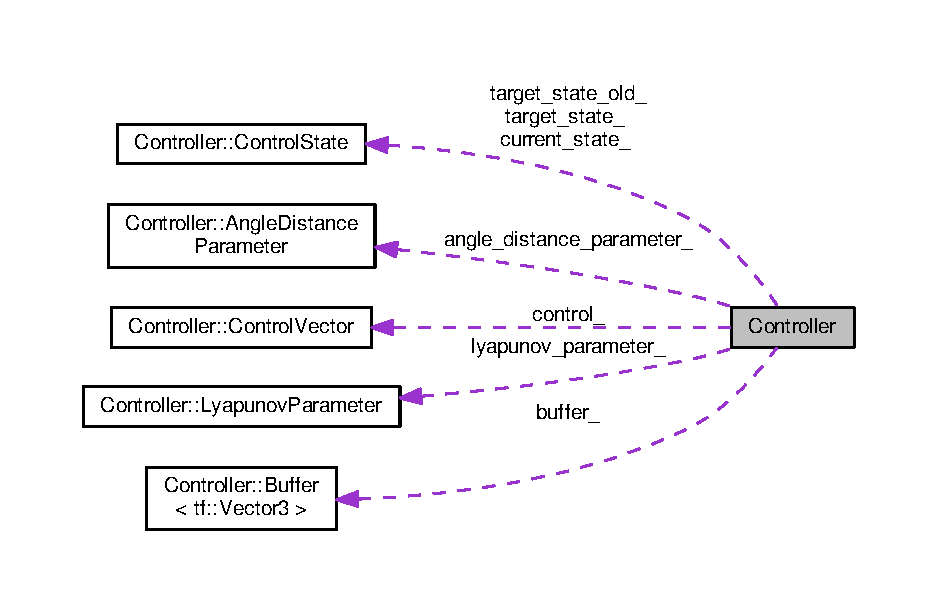
\includegraphics[width=350pt]{classController__coll__graph}
\end{center}
\end{figure}
\subsection*{Classes}
\begin{DoxyCompactItemize}
\item 
struct \hyperlink{structController_1_1ControlState}{Control\+State}
\begin{DoxyCompactList}\small\item\em Holds the System state combined by the pose of the system, the cartesian velocity and the angular velocity. \end{DoxyCompactList}\item 
struct \hyperlink{structController_1_1ControlVector}{Control\+Vector}
\begin{DoxyCompactList}\small\item\em A struct that holds linear and angular velocity of the Robot since this are the control variable for kinematic tracking control. \end{DoxyCompactList}\item 
struct \hyperlink{structController_1_1LyapunovParameter}{Lyapunov\+Parameter}
\begin{DoxyCompactList}\small\item\em Specifies the parameters needed for the lyapunov based control law. \end{DoxyCompactList}\end{DoxyCompactItemize}
\subsection*{Public Types}
\begin{DoxyCompactItemize}
\item 
enum \hyperlink{classController_aa6d956c4c220461a4152415ffa78690a}{Controller\+Type} \{ \hyperlink{classController_aa6d956c4c220461a4152415ffa78690aad2e9073ef821965020410686a3c89483}{pseudo\+\_\+inverse} =1, 
\hyperlink{classController_aa6d956c4c220461a4152415ffa78690aaed0e850e561d54619d85f32c37f5bfab}{lypanov} =2, 
\hyperlink{classController_aa6d956c4c220461a4152415ffa78690aa7ab0ee34114a951d4491d6eb73500cdc}{angle\+\_\+distance} =3
 \}\begin{DoxyCompactList}\small\item\em Specifies the different implemented control laws. \end{DoxyCompactList}
\item 
typedef tf\+::\+Vector3 \hyperlink{classController_a7ab3d947ee649f6bac652de6a00e8148}{Velocity\+Cartesian}\hypertarget{classController_a7ab3d947ee649f6bac652de6a00e8148}{}\label{classController_a7ab3d947ee649f6bac652de6a00e8148}

\begin{DoxyCompactList}\small\item\em Defines Velocity\+Cartesian wich is used to stores cartesian defined velocities. \end{DoxyCompactList}\item 
typedef tf\+::\+Vector3 \hyperlink{classController_a1b8b4035525237f0112b81d44a23da2c}{Position\+Cartesian}\hypertarget{classController_a1b8b4035525237f0112b81d44a23da2c}{}\label{classController_a1b8b4035525237f0112b81d44a23da2c}

\begin{DoxyCompactList}\small\item\em Defines Position\+Cartesian wich is used to store a cartesian defined position. \end{DoxyCompactList}\item 
typedef tf\+::\+Transform \hyperlink{classController_a75a1e2f93842f65d1263f7d3c2fd8898}{Control\+Difference}\hypertarget{classController_a75a1e2f93842f65d1263f7d3c2fd8898}{}\label{classController_a75a1e2f93842f65d1263f7d3c2fd8898}

\begin{DoxyCompactList}\small\item\em Defines Control\+Difference wich is a transformation from the current state in the target state. \end{DoxyCompactList}\item 
typedef \hyperlink{structController_1_1ControlVector}{Control\+Vector} \hyperlink{classController_a6849bee332c04d67ac6f3052cccd2669}{Velocity\+Eulerian}\hypertarget{classController_a6849bee332c04d67ac6f3052cccd2669}{}\label{classController_a6849bee332c04d67ac6f3052cccd2669}

\begin{DoxyCompactList}\small\item\em Defines Velocity\+Eulerian wich is used to store Velocities wich are defined locally in the moved base system. \end{DoxyCompactList}\end{DoxyCompactItemize}
\subsection*{Public Member Functions}
\begin{DoxyCompactItemize}
\item 
\hyperlink{classController_a7341f9092e1977cdd2a1492c4422c019}{Controller} (ros\+::\+Node\+Handle \&\hyperlink{classController_a24e3d3c2536f6ed29018bad1fd53dae2}{nh})
\begin{DoxyCompactList}\small\item\em Construct a new \hyperlink{classController}{Controller} object. \end{DoxyCompactList}\item 
\hyperlink{classController_a0ab87934c4f7a266cfdb86e0f36bc1b5}{$\sim$\+Controller} ()\hypertarget{classController_a0ab87934c4f7a266cfdb86e0f36bc1b5}{}\label{classController_a0ab87934c4f7a266cfdb86e0f36bc1b5}

\begin{DoxyCompactList}\small\item\em Destroy the \hyperlink{classController}{Controller} object. \end{DoxyCompactList}\item 
void \hyperlink{classController_a177d0d6cd7cdb7784ae9c506debfa2c6}{set\+Name} (std\+::string \hyperlink{classController_af81f22d8b64d915769acfb8e8d89e0c8}{name})
\begin{DoxyCompactList}\small\item\em Set the name of object. \end{DoxyCompactList}\item 
void \hyperlink{classController_a156a66bd7cd6340106accbb982b6238b}{set\+Reference} (double x, double y, double z, double angle)
\begin{DoxyCompactList}\small\item\em Set the reference of the mobile robot to be controlled from a global frame. \end{DoxyCompactList}\item 
void \hyperlink{classController_ae86ed49c452a9e94568312ef743aa082}{set\+Reference} (std\+::vector$<$ double $>$ coord, double angle)
\begin{DoxyCompactList}\small\item\em Set the reference of the mobile robot to be controlled from a global frame. \end{DoxyCompactList}\item 
void \hyperlink{classController_adf25339eadd9b31bc1d6b3e47395942e}{set\+World\+Frame} (std\+::string frame)
\begin{DoxyCompactList}\small\item\em Set the world frame name all references are given in. \end{DoxyCompactList}\item 
void \hyperlink{classController_a25202c469ad65696761242dce4e28d76}{set\+Type} (\hyperlink{classController_aa6d956c4c220461a4152415ffa78690a}{Controller\+::\+Controller\+Type} \hyperlink{classController_a17792cff397dc69baca568c7d03f2fc8}{type})
\begin{DoxyCompactList}\small\item\em Sets the type of the used control law. \end{DoxyCompactList}\item 
void \hyperlink{classController_abda96416fab439c188ef494a2b2a0c8e}{set\+Lyapunov} (\hyperlink{structController_1_1LyapunovParameter}{Controller\+::\+Lyapunov\+Parameter} param)
\begin{DoxyCompactList}\small\item\em Sets the parameter of the lyapunov control law. \end{DoxyCompactList}\item 
void \hyperlink{classController_a1f77caed7a7951ca2f4cf7928f88669d}{set\+Lyapunov} (std\+::vector$<$ float $>$ param)
\begin{DoxyCompactList}\small\item\em Sets the parameter of the lyapunov control law. \end{DoxyCompactList}\item 
virtual void \hyperlink{classController_a59e60885d5307979faf477435507069a}{load\+Parameter} ()\hypertarget{classController_a59e60885d5307979faf477435507069a}{}\label{classController_a59e60885d5307979faf477435507069a}

\begin{DoxyCompactList}\small\item\em Loading parameter for a specified \hyperlink{classController}{Controller}. Empty for \hyperlink{classController}{Controller} base class and implemented in inheriting classes. \end{DoxyCompactList}\item 
void \hyperlink{classController_a55c77d2e41634c9b21543647f74eec4c}{load} ()\hypertarget{classController_a55c77d2e41634c9b21543647f74eec4c}{}\label{classController_a55c77d2e41634c9b21543647f74eec4c}

\begin{DoxyCompactList}\small\item\em Loading of R\+OS parameterset for this controller. \end{DoxyCompactList}\item 
void \hyperlink{classController_aa0ea10adc7a81124663fb01693acef17}{link\+Current\+Odom} (std\+::string topic\+\_\+name)
\begin{DoxyCompactList}\small\item\em Links the current odometry topic to the controller. At this topic the current odomotry of the robot must be published. \end{DoxyCompactList}\item 
void \hyperlink{classController_a633d84f97952551654ee70acc31810c6}{link\+Target\+Odom} (std\+::string topic\+\_\+name)
\begin{DoxyCompactList}\small\item\em Links the target/desired odometry topic to the controller. At this topic the desired odometry is published. \end{DoxyCompactList}\item 
void \hyperlink{classController_a7bde6b39b2b2cccb1dd866841f672f99}{link\+Output\+Velocity} (std\+::string topic\+\_\+name)
\begin{DoxyCompactList}\small\item\em Links the output velocity of the controller to a given topic. \end{DoxyCompactList}\item 
void \hyperlink{classController_a6412541600d7444f00f8e48cea0ed024}{link\+Output\+Control\+Data} (std\+::string topic\+\_\+name)
\begin{DoxyCompactList}\small\item\em Links the meta data of the controller to a given topic. \end{DoxyCompactList}\item 
virtual void \hyperlink{classController_a9bf99e0d40660b832c2e70691e9f0a1c}{current\+Odom\+Callback} (nav\+\_\+msgs\+::\+Odometry msg)
\begin{DoxyCompactList}\small\item\em Callback for incoming odometry data for the current robot odometry. \end{DoxyCompactList}\item 
virtual void \hyperlink{classController_a77f138b6a3699c21cf904041e7e19820}{target\+Odom\+Callback} (nav\+\_\+msgs\+::\+Odometry msg)
\begin{DoxyCompactList}\small\item\em Callback for incoming state data for the target odometry of the robot. This is overloaded by child classes. \end{DoxyCompactList}\item 
struct \hyperlink{structController_1_1ControlVector}{Control\+Vector} \hyperlink{classController_a5342dd66c1228e651e569d9b1c31d82e}{calc\+Lyapunov} (\hyperlink{structController_1_1LyapunovParameter}{Lyapunov\+Parameter} parameter, \hyperlink{classController_a6849bee332c04d67ac6f3052cccd2669}{Velocity\+Eulerian} desired, tf\+::\+Transform relative)
\item 
void \hyperlink{classController_abe0a6e0155a0b159efe425e635d3ae76}{execute} (const ros\+::\+Timer\+Event \&ev)\hypertarget{classController_abe0a6e0155a0b159efe425e635d3ae76}{}\label{classController_abe0a6e0155a0b159efe425e635d3ae76}

\begin{DoxyCompactList}\small\item\em Scope of the controller that is called in control frequence. \end{DoxyCompactList}\item 
void \hyperlink{classController_ab5515748f1b0c82f015e039c817ee5f7}{reset} ()\hypertarget{classController_ab5515748f1b0c82f015e039c817ee5f7}{}\label{classController_ab5515748f1b0c82f015e039c817ee5f7}

\begin{DoxyCompactList}\small\item\em Resetting controller to initial state. \end{DoxyCompactList}\item 
bool \hyperlink{classController_a140aa1ee895337d776f88682640c0746}{srv\+Reset} (std\+\_\+srvs\+::\+Empty\+Request \&req, std\+\_\+srvs\+::\+Empty\+Response \&res)
\begin{DoxyCompactList}\small\item\em Service procedure for resetting the \hyperlink{classController}{Controller}. \end{DoxyCompactList}\item 
void \hyperlink{classController_a753fe3680abc7c9ba3040f6fcb638ac2}{control\+State2control\+State\+Msg} (\hyperlink{structController_1_1ControlState}{Control\+State} \&state, multi\+\_\+robot\+\_\+msgs\+::\+Control\+State \&msg)
\begin{DoxyCompactList}\small\item\em Converts \hyperlink{structController_1_1ControlState}{Control\+State} struct to a C\+Ontrol state message. \end{DoxyCompactList}\item 
void \hyperlink{classController_a866cee7328e1318e118c884a850a0e34}{control\+Difference2control\+Difference\+Msg} (\hyperlink{classController_a75a1e2f93842f65d1263f7d3c2fd8898}{Control\+Difference} \&difference, multi\+\_\+robot\+\_\+msgs\+::\+Control\+Difference \&msg)
\begin{DoxyCompactList}\small\item\em Converts Control\+Difference struct to a C\+Ontrol state message. \end{DoxyCompactList}\item 
void \hyperlink{classController_a06c1aab700c5918b76e33c35f3da8ea8}{control\+Vector2control\+Vector\+Msg} (\hyperlink{structController_1_1ControlVector}{Control\+Vector} \&control, multi\+\_\+robot\+\_\+msgs\+::\+Control\+Vector \&msg)
\begin{DoxyCompactList}\small\item\em Converts \hyperlink{structController_1_1ControlVector}{Control\+Vector} struct to a C\+Ontrol state message. \end{DoxyCompactList}\end{DoxyCompactItemize}
\subsection*{Protected Attributes}
\begin{DoxyCompactItemize}
\item 
ros\+::\+Node\+Handle \hyperlink{classController_a24e3d3c2536f6ed29018bad1fd53dae2}{nh}\hypertarget{classController_a24e3d3c2536f6ed29018bad1fd53dae2}{}\label{classController_a24e3d3c2536f6ed29018bad1fd53dae2}

\begin{DoxyCompactList}\small\item\em Node Handle. \end{DoxyCompactList}\item 
tf\+::\+Transform\+Listener $\ast$ \hyperlink{classController_afea373f808d583e4ad613f119439a8f5}{listener}\hypertarget{classController_afea373f808d583e4ad613f119439a8f5}{}\label{classController_afea373f808d583e4ad613f119439a8f5}

\begin{DoxyCompactList}\small\item\em Listener for any transformation. \end{DoxyCompactList}\item 
std\+::string \hyperlink{classController_ae01171e69d9b735e44964662275fc77c}{world\+\_\+frame}\hypertarget{classController_ae01171e69d9b735e44964662275fc77c}{}\label{classController_ae01171e69d9b735e44964662275fc77c}

\begin{DoxyCompactList}\small\item\em Name of the world frame. \end{DoxyCompactList}\item 
\hyperlink{structController_1_1ControlState}{Control\+State} \hyperlink{classController_aaca736f25e7da33272ded507e0c8057f}{current\+\_\+state\+\_\+}\hypertarget{classController_aaca736f25e7da33272ded507e0c8057f}{}\label{classController_aaca736f25e7da33272ded507e0c8057f}

\begin{DoxyCompactList}\small\item\em The current state of the robot. \end{DoxyCompactList}\item 
\hyperlink{structController_1_1ControlState}{Control\+State} \hyperlink{classController_a8412c8448970cf820f932cff02d69d33}{target\+\_\+state\+\_\+}\hypertarget{classController_a8412c8448970cf820f932cff02d69d33}{}\label{classController_a8412c8448970cf820f932cff02d69d33}

\begin{DoxyCompactList}\small\item\em The target state of the robot. \end{DoxyCompactList}\item 
\hyperlink{classController_a75a1e2f93842f65d1263f7d3c2fd8898}{Control\+Difference} \hyperlink{classController_afe3b54c59a80046661f0030a573539d7}{control\+\_\+dif\+\_\+}\hypertarget{classController_afe3b54c59a80046661f0030a573539d7}{}\label{classController_afe3b54c59a80046661f0030a573539d7}

\begin{DoxyCompactList}\small\item\em Transformation from current configuration to target configuration. \end{DoxyCompactList}\item 
\hyperlink{structController_1_1ControlVector}{Control\+Vector} \hyperlink{classController_aaafcd892e9e6080e839a1348a7ef40db}{control\+\_\+}\hypertarget{classController_aaafcd892e9e6080e839a1348a7ef40db}{}\label{classController_aaafcd892e9e6080e839a1348a7ef40db}

\begin{DoxyCompactList}\small\item\em The calculated control vector. \end{DoxyCompactList}\item 
tf\+::\+Transform \hyperlink{classController_aa713beca2ef8152d273bbc6fc38f7fc8}{world2reference\+\_\+}\hypertarget{classController_aa713beca2ef8152d273bbc6fc38f7fc8}{}\label{classController_aa713beca2ef8152d273bbc6fc38f7fc8}

\begin{DoxyCompactList}\small\item\em Transformation from a world to the controllers refrence frame. \end{DoxyCompactList}\end{DoxyCompactItemize}
\subsection*{Private Member Functions}
\begin{DoxyCompactItemize}
\item 
void \hyperlink{classController_ae6859e3a43be2fa31cb82ace3954e746}{publish} ()\hypertarget{classController_ae6859e3a43be2fa31cb82ace3954e746}{}\label{classController_ae6859e3a43be2fa31cb82ace3954e746}

\begin{DoxyCompactList}\small\item\em Publish all outgoing data. \end{DoxyCompactList}\item 
void \hyperlink{classController_a8509c67c73d26e981ef0972f44dc73ca}{publish\+\_\+refrence} ()\hypertarget{classController_a8509c67c73d26e981ef0972f44dc73ca}{}\label{classController_a8509c67c73d26e981ef0972f44dc73ca}

\begin{DoxyCompactList}\small\item\em Adding the world frame. Broadcastes a world frame respectiveliy the robot reference frame expressed in world coordinates. \end{DoxyCompactList}\end{DoxyCompactItemize}
\subsection*{Private Attributes}
\begin{DoxyCompactItemize}
\item 
ros\+::\+Publisher \hyperlink{classController_a2ff92c110ca7f28bdd702229a1295505}{pub\+\_\+cmd\+\_\+vel}\hypertarget{classController_a2ff92c110ca7f28bdd702229a1295505}{}\label{classController_a2ff92c110ca7f28bdd702229a1295505}

\begin{DoxyCompactList}\small\item\em publisher object for velocity outoput topic \end{DoxyCompactList}\item 
ros\+::\+Publisher \hyperlink{classController_a6abeaf23d1c17d6af6eecf7d1479fe31}{pub\+\_\+state\+\_\+out}\hypertarget{classController_a6abeaf23d1c17d6af6eecf7d1479fe31}{}\label{classController_a6abeaf23d1c17d6af6eecf7d1479fe31}

\begin{DoxyCompactList}\small\item\em publisher object for state output topic \end{DoxyCompactList}\item 
ros\+::\+Publisher \hyperlink{classController_afde3eefcf7ac040b2a38a8d1e95a6077}{pub\+\_\+control\+\_\+data}\hypertarget{classController_afde3eefcf7ac040b2a38a8d1e95a6077}{}\label{classController_afde3eefcf7ac040b2a38a8d1e95a6077}

\begin{DoxyCompactList}\small\item\em publisher object for control difference topic \end{DoxyCompactList}\item 
ros\+::\+Subscriber \hyperlink{classController_a855093341ac8afa84efd841654fedaf5}{sub\+\_\+odom\+\_\+current}\hypertarget{classController_a855093341ac8afa84efd841654fedaf5}{}\label{classController_a855093341ac8afa84efd841654fedaf5}

\begin{DoxyCompactList}\small\item\em Subscriber object for odometry. \end{DoxyCompactList}\item 
ros\+::\+Subscriber \hyperlink{classController_a7c21cd887b80a3ebceae1e5e320c6ad8}{sub\+\_\+odom\+\_\+target}\hypertarget{classController_a7c21cd887b80a3ebceae1e5e320c6ad8}{}\label{classController_a7c21cd887b80a3ebceae1e5e320c6ad8}

\begin{DoxyCompactList}\small\item\em Subscriber object for target odometry topic. \end{DoxyCompactList}\item 
ros\+::\+Timer \hyperlink{classController_a96e34ca6ebe5b7c8035982ff98270f4b}{time\+\_\+scope\+\_\+}\hypertarget{classController_a96e34ca6ebe5b7c8035982ff98270f4b}{}\label{classController_a96e34ca6ebe5b7c8035982ff98270f4b}

\begin{DoxyCompactList}\small\item\em Timer for control scope. \end{DoxyCompactList}\item 
ros\+::\+Service\+Server \hyperlink{classController_ae981013bac649b6310e924b6a126bc40}{reset\+\_\+service}\hypertarget{classController_ae981013bac649b6310e924b6a126bc40}{}\label{classController_ae981013bac649b6310e924b6a126bc40}

\begin{DoxyCompactList}\small\item\em Service for resetting the controller. \end{DoxyCompactList}\item 
std\+::string \hyperlink{classController_af81f22d8b64d915769acfb8e8d89e0c8}{name}\hypertarget{classController_af81f22d8b64d915769acfb8e8d89e0c8}{}\label{classController_af81f22d8b64d915769acfb8e8d89e0c8}

\begin{DoxyCompactList}\small\item\em Name of the node respective \hyperlink{classController}{Controller}. \end{DoxyCompactList}\item 
\hyperlink{structController_1_1LyapunovParameter}{Lyapunov\+Parameter} \hyperlink{classController_a8069db2319ff64d65607b1aa897d3069}{lyapunov\+\_\+parameter}\hypertarget{classController_a8069db2319ff64d65607b1aa897d3069}{}\label{classController_a8069db2319ff64d65607b1aa897d3069}

\begin{DoxyCompactList}\small\item\em Parameter set for lyapunov determinations. \end{DoxyCompactList}\item 
\hyperlink{classController_aa6d956c4c220461a4152415ffa78690a}{Controller\+Type} \hyperlink{classController_a17792cff397dc69baca568c7d03f2fc8}{type}\hypertarget{classController_a17792cff397dc69baca568c7d03f2fc8}{}\label{classController_a17792cff397dc69baca568c7d03f2fc8}

\begin{DoxyCompactList}\small\item\em Type of control algorythm that is used. \end{DoxyCompactList}\item 
bool \hyperlink{classController_a4e0e569456498e5670a48244c22cafc9}{loaded\+\_\+parameter}\hypertarget{classController_a4e0e569456498e5670a48244c22cafc9}{}\label{classController_a4e0e569456498e5670a48244c22cafc9}

\begin{DoxyCompactList}\small\item\em Flag if parameter were loaded from the parameter server. \end{DoxyCompactList}\end{DoxyCompactItemize}


\subsection{Detailed Description}
Provides a easy to use implementation of a generic mobile robot controller. 

\subsection{Member Enumeration Documentation}
\index{Controller@{Controller}!Controller\+Type@{Controller\+Type}}
\index{Controller\+Type@{Controller\+Type}!Controller@{Controller}}
\subsubsection[{\texorpdfstring{Controller\+Type}{ControllerType}}]{\setlength{\rightskip}{0pt plus 5cm}enum {\bf Controller\+::\+Controller\+Type}}\hypertarget{classController_aa6d956c4c220461a4152415ffa78690a}{}\label{classController_aa6d956c4c220461a4152415ffa78690a}


Specifies the different implemented control laws. 

\begin{Desc}
\item[Enumerator]\par
\begin{description}
\index{pseudo\+\_\+inverse@{pseudo\+\_\+inverse}!Controller@{Controller}}\index{Controller@{Controller}!pseudo\+\_\+inverse@{pseudo\+\_\+inverse}}\item[{\em 
pseudo\+\_\+inverse\hypertarget{classController_aa6d956c4c220461a4152415ffa78690aad2e9073ef821965020410686a3c89483}{}\label{classController_aa6d956c4c220461a4152415ffa78690aad2e9073ef821965020410686a3c89483}
}]Control law is based on pseudo inveres the input for generate a output (least squares optimisation) \index{lypanov@{lypanov}!Controller@{Controller}}\index{Controller@{Controller}!lypanov@{lypanov}}\item[{\em 
lypanov\hypertarget{classController_aa6d956c4c220461a4152415ffa78690aaed0e850e561d54619d85f32c37f5bfab}{}\label{classController_aa6d956c4c220461a4152415ffa78690aaed0e850e561d54619d85f32c37f5bfab}
}]Control law is based on the lyapunov approache. Output is determined from a lyapunov stable function \index{angle\+\_\+distance@{angle\+\_\+distance}!Controller@{Controller}}\index{Controller@{Controller}!angle\+\_\+distance@{angle\+\_\+distance}}\item[{\em 
angle\+\_\+distance\hypertarget{classController_aa6d956c4c220461a4152415ffa78690aa7ab0ee34114a951d4491d6eb73500cdc}{}\label{classController_aa6d956c4c220461a4152415ffa78690aa7ab0ee34114a951d4491d6eb73500cdc}
}]Control law based on linear approach in angle and distance respectively \end{description}
\end{Desc}


\subsection{Constructor \& Destructor Documentation}
\index{Controller@{Controller}!Controller@{Controller}}
\index{Controller@{Controller}!Controller@{Controller}}
\subsubsection[{\texorpdfstring{Controller(ros\+::\+Node\+Handle \&nh)}{Controller(ros::NodeHandle &nh)}}]{\setlength{\rightskip}{0pt plus 5cm}Controller\+::\+Controller (
\begin{DoxyParamCaption}
\item[{ros\+::\+Node\+Handle \&}]{nh}
\end{DoxyParamCaption}
)}\hypertarget{classController_a7341f9092e1977cdd2a1492c4422c019}{}\label{classController_a7341f9092e1977cdd2a1492c4422c019}


Construct a new \hyperlink{classController}{Controller} object. 


\begin{DoxyParams}{Parameters}
{\em nh} & Ros nodehandle for managing namespaces and ros functionality within the controller object \\
\hline
\end{DoxyParams}


\subsection{Member Function Documentation}
\index{Controller@{Controller}!calc\+Lyapunov@{calc\+Lyapunov}}
\index{calc\+Lyapunov@{calc\+Lyapunov}!Controller@{Controller}}
\subsubsection[{\texorpdfstring{calc\+Lyapunov(\+Lyapunov\+Parameter parameter, Velocity\+Eulerian desired, tf\+::\+Transform relative)}{calcLyapunov(LyapunovParameter parameter, VelocityEulerian desired, tf::Transform relative)}}]{\setlength{\rightskip}{0pt plus 5cm}struct {\bf Controller\+::\+Control\+Vector} Controller\+::calc\+Lyapunov (
\begin{DoxyParamCaption}
\item[{{\bf Lyapunov\+Parameter}}]{parameter, }
\item[{{\bf Velocity\+Eulerian}}]{desired, }
\item[{tf\+::\+Transform}]{relative}
\end{DoxyParamCaption}
)}\hypertarget{classController_a5342dd66c1228e651e569d9b1c31d82e}{}\label{classController_a5342dd66c1228e651e569d9b1c31d82e}

\begin{DoxyParams}{Parameters}
{\em parameter} & Set of lyapunov parameter for calculating the control vector \\
\hline
{\em desired} & Desired velocities in eulerian description (moved base). Contains angular and linear velocity \\
\hline
{\em relative} & Transformation from current to target state \\
\hline
\end{DoxyParams}
\begin{DoxyReturn}{Returns}
\hyperlink{structController_1_1ControlVector}{Control\+Vector} 
\end{DoxyReturn}
\index{Controller@{Controller}!control\+Difference2control\+Difference\+Msg@{control\+Difference2control\+Difference\+Msg}}
\index{control\+Difference2control\+Difference\+Msg@{control\+Difference2control\+Difference\+Msg}!Controller@{Controller}}
\subsubsection[{\texorpdfstring{control\+Difference2control\+Difference\+Msg(\+Control\+Difference \&difference, multi\+\_\+robot\+\_\+msgs\+::\+Control\+Difference \&msg)}{controlDifference2controlDifferenceMsg(ControlDifference &difference, multi_robot_msgs::ControlDifference &msg)}}]{\setlength{\rightskip}{0pt plus 5cm}void Controller\+::control\+Difference2control\+Difference\+Msg (
\begin{DoxyParamCaption}
\item[{{\bf Control\+Difference} \&}]{difference, }
\item[{multi\+\_\+robot\+\_\+msgs\+::\+Control\+Difference \&}]{msg}
\end{DoxyParamCaption}
)}\hypertarget{classController_a866cee7328e1318e118c884a850a0e34}{}\label{classController_a866cee7328e1318e118c884a850a0e34}


Converts Control\+Difference struct to a C\+Ontrol state message. 


\begin{DoxyParams}{Parameters}
{\em difference} & Control\+Difference to be converted \\
\hline
{\em msg} & Referenze to the msg the conversion is stored in \\
\hline
\end{DoxyParams}
\index{Controller@{Controller}!control\+State2control\+State\+Msg@{control\+State2control\+State\+Msg}}
\index{control\+State2control\+State\+Msg@{control\+State2control\+State\+Msg}!Controller@{Controller}}
\subsubsection[{\texorpdfstring{control\+State2control\+State\+Msg(\+Control\+State \&state, multi\+\_\+robot\+\_\+msgs\+::\+Control\+State \&msg)}{controlState2controlStateMsg(ControlState &state, multi_robot_msgs::ControlState &msg)}}]{\setlength{\rightskip}{0pt plus 5cm}void Controller\+::control\+State2control\+State\+Msg (
\begin{DoxyParamCaption}
\item[{{\bf Controller\+::\+Control\+State} \&}]{state, }
\item[{multi\+\_\+robot\+\_\+msgs\+::\+Control\+State \&}]{msg}
\end{DoxyParamCaption}
)}\hypertarget{classController_a753fe3680abc7c9ba3040f6fcb638ac2}{}\label{classController_a753fe3680abc7c9ba3040f6fcb638ac2}


Converts \hyperlink{structController_1_1ControlState}{Control\+State} struct to a C\+Ontrol state message. 


\begin{DoxyParams}{Parameters}
{\em state} & Control state to be converted \\
\hline
{\em msg} & Referenze to the msg the conversion is stored in \\
\hline
\end{DoxyParams}
\index{Controller@{Controller}!control\+Vector2control\+Vector\+Msg@{control\+Vector2control\+Vector\+Msg}}
\index{control\+Vector2control\+Vector\+Msg@{control\+Vector2control\+Vector\+Msg}!Controller@{Controller}}
\subsubsection[{\texorpdfstring{control\+Vector2control\+Vector\+Msg(\+Control\+Vector \&control, multi\+\_\+robot\+\_\+msgs\+::\+Control\+Vector \&msg)}{controlVector2controlVectorMsg(ControlVector &control, multi_robot_msgs::ControlVector &msg)}}]{\setlength{\rightskip}{0pt plus 5cm}void Controller\+::control\+Vector2control\+Vector\+Msg (
\begin{DoxyParamCaption}
\item[{{\bf Control\+Vector} \&}]{control, }
\item[{multi\+\_\+robot\+\_\+msgs\+::\+Control\+Vector \&}]{msg}
\end{DoxyParamCaption}
)}\hypertarget{classController_a06c1aab700c5918b76e33c35f3da8ea8}{}\label{classController_a06c1aab700c5918b76e33c35f3da8ea8}


Converts \hyperlink{structController_1_1ControlVector}{Control\+Vector} struct to a C\+Ontrol state message. 


\begin{DoxyParams}{Parameters}
{\em control} & \hyperlink{structController_1_1ControlVector}{Control\+Vector} to be converted \\
\hline
{\em msg} & Referenze to the msg the conversion is stored in \\
\hline
\end{DoxyParams}
\index{Controller@{Controller}!current\+Odom\+Callback@{current\+Odom\+Callback}}
\index{current\+Odom\+Callback@{current\+Odom\+Callback}!Controller@{Controller}}
\subsubsection[{\texorpdfstring{current\+Odom\+Callback(nav\+\_\+msgs\+::\+Odometry msg)}{currentOdomCallback(nav_msgs::Odometry msg)}}]{\setlength{\rightskip}{0pt plus 5cm}void Controller\+::current\+Odom\+Callback (
\begin{DoxyParamCaption}
\item[{nav\+\_\+msgs\+::\+Odometry}]{msg}
\end{DoxyParamCaption}
)\hspace{0.3cm}{\ttfamily [virtual]}}\hypertarget{classController_a9bf99e0d40660b832c2e70691e9f0a1c}{}\label{classController_a9bf99e0d40660b832c2e70691e9f0a1c}


Callback for incoming odometry data for the current robot odometry. 


\begin{DoxyParams}{Parameters}
{\em msg} & Incoming message \\
\hline
\end{DoxyParams}
\index{Controller@{Controller}!link\+Current\+Odom@{link\+Current\+Odom}}
\index{link\+Current\+Odom@{link\+Current\+Odom}!Controller@{Controller}}
\subsubsection[{\texorpdfstring{link\+Current\+Odom(std\+::string topic\+\_\+name)}{linkCurrentOdom(std::string topic_name)}}]{\setlength{\rightskip}{0pt plus 5cm}void Controller\+::link\+Current\+Odom (
\begin{DoxyParamCaption}
\item[{std\+::string}]{topic\+\_\+name}
\end{DoxyParamCaption}
)}\hypertarget{classController_aa0ea10adc7a81124663fb01693acef17}{}\label{classController_aa0ea10adc7a81124663fb01693acef17}


Links the current odometry topic to the controller. At this topic the current odomotry of the robot must be published. 


\begin{DoxyParams}{Parameters}
{\em topic\+\_\+name} & Name of the topic \\
\hline
\end{DoxyParams}
\index{Controller@{Controller}!link\+Output\+Control\+Data@{link\+Output\+Control\+Data}}
\index{link\+Output\+Control\+Data@{link\+Output\+Control\+Data}!Controller@{Controller}}
\subsubsection[{\texorpdfstring{link\+Output\+Control\+Data(std\+::string topic\+\_\+name)}{linkOutputControlData(std::string topic_name)}}]{\setlength{\rightskip}{0pt plus 5cm}void Controller\+::link\+Output\+Control\+Data (
\begin{DoxyParamCaption}
\item[{std\+::string}]{topic\+\_\+name}
\end{DoxyParamCaption}
)}\hypertarget{classController_a6412541600d7444f00f8e48cea0ed024}{}\label{classController_a6412541600d7444f00f8e48cea0ed024}


Links the meta data of the controller to a given topic. 


\begin{DoxyParams}{Parameters}
{\em topic\+\_\+name} & Name of the topic \\
\hline
\end{DoxyParams}
\index{Controller@{Controller}!link\+Output\+Velocity@{link\+Output\+Velocity}}
\index{link\+Output\+Velocity@{link\+Output\+Velocity}!Controller@{Controller}}
\subsubsection[{\texorpdfstring{link\+Output\+Velocity(std\+::string topic\+\_\+name)}{linkOutputVelocity(std::string topic_name)}}]{\setlength{\rightskip}{0pt plus 5cm}void Controller\+::link\+Output\+Velocity (
\begin{DoxyParamCaption}
\item[{std\+::string}]{topic\+\_\+name}
\end{DoxyParamCaption}
)}\hypertarget{classController_a7bde6b39b2b2cccb1dd866841f672f99}{}\label{classController_a7bde6b39b2b2cccb1dd866841f672f99}


Links the output velocity of the controller to a given topic. 

O\+U\+T\+P\+U\+TS.


\begin{DoxyParams}{Parameters}
{\em topic\+\_\+name} & Name of the topic \\
\hline
\end{DoxyParams}
\index{Controller@{Controller}!link\+Target\+Odom@{link\+Target\+Odom}}
\index{link\+Target\+Odom@{link\+Target\+Odom}!Controller@{Controller}}
\subsubsection[{\texorpdfstring{link\+Target\+Odom(std\+::string topic\+\_\+name)}{linkTargetOdom(std::string topic_name)}}]{\setlength{\rightskip}{0pt plus 5cm}void Controller\+::link\+Target\+Odom (
\begin{DoxyParamCaption}
\item[{std\+::string}]{topic\+\_\+name}
\end{DoxyParamCaption}
)}\hypertarget{classController_a633d84f97952551654ee70acc31810c6}{}\label{classController_a633d84f97952551654ee70acc31810c6}


Links the target/desired odometry topic to the controller. At this topic the desired odometry is published. 


\begin{DoxyParams}{Parameters}
{\em topic\+\_\+name} & Name of the topic \\
\hline
\end{DoxyParams}
\index{Controller@{Controller}!set\+Lyapunov@{set\+Lyapunov}}
\index{set\+Lyapunov@{set\+Lyapunov}!Controller@{Controller}}
\subsubsection[{\texorpdfstring{set\+Lyapunov(\+Controller\+::\+Lyapunov\+Parameter param)}{setLyapunov(Controller::LyapunovParameter param)}}]{\setlength{\rightskip}{0pt plus 5cm}void Controller\+::set\+Lyapunov (
\begin{DoxyParamCaption}
\item[{{\bf Controller\+::\+Lyapunov\+Parameter}}]{param}
\end{DoxyParamCaption}
)}\hypertarget{classController_abda96416fab439c188ef494a2b2a0c8e}{}\label{classController_abda96416fab439c188ef494a2b2a0c8e}


Sets the parameter of the lyapunov control law. 


\begin{DoxyParams}{Parameters}
{\em param} & Parameterset as defined in lyapunov struct \\
\hline
\end{DoxyParams}
\index{Controller@{Controller}!set\+Lyapunov@{set\+Lyapunov}}
\index{set\+Lyapunov@{set\+Lyapunov}!Controller@{Controller}}
\subsubsection[{\texorpdfstring{set\+Lyapunov(std\+::vector$<$ float $>$ param)}{setLyapunov(std::vector< float > param)}}]{\setlength{\rightskip}{0pt plus 5cm}void Controller\+::set\+Lyapunov (
\begin{DoxyParamCaption}
\item[{std\+::vector$<$ float $>$}]{param}
\end{DoxyParamCaption}
)}\hypertarget{classController_a1f77caed7a7951ca2f4cf7928f88669d}{}\label{classController_a1f77caed7a7951ca2f4cf7928f88669d}


Sets the parameter of the lyapunov control law. 


\begin{DoxyParams}{Parameters}
{\em param} & vector of given parameters \mbox{[}kx,ky,ktheta,vd,omega\mbox{]} \\
\hline
\end{DoxyParams}
\index{Controller@{Controller}!set\+Name@{set\+Name}}
\index{set\+Name@{set\+Name}!Controller@{Controller}}
\subsubsection[{\texorpdfstring{set\+Name(std\+::string name)}{setName(std::string name)}}]{\setlength{\rightskip}{0pt plus 5cm}void Controller\+::set\+Name (
\begin{DoxyParamCaption}
\item[{std\+::string}]{name}
\end{DoxyParamCaption}
)}\hypertarget{classController_a177d0d6cd7cdb7784ae9c506debfa2c6}{}\label{classController_a177d0d6cd7cdb7784ae9c506debfa2c6}


Set the name of object. 


\begin{DoxyParams}{Parameters}
{\em name} & Name to be set \\
\hline
\end{DoxyParams}
\index{Controller@{Controller}!set\+Reference@{set\+Reference}}
\index{set\+Reference@{set\+Reference}!Controller@{Controller}}
\subsubsection[{\texorpdfstring{set\+Reference(double x, double y, double z, double angle)}{setReference(double x, double y, double z, double angle)}}]{\setlength{\rightskip}{0pt plus 5cm}void Controller\+::set\+Reference (
\begin{DoxyParamCaption}
\item[{double}]{x, }
\item[{double}]{y, }
\item[{double}]{z, }
\item[{double}]{angle}
\end{DoxyParamCaption}
)}\hypertarget{classController_a156a66bd7cd6340106accbb982b6238b}{}\label{classController_a156a66bd7cd6340106accbb982b6238b}


Set the reference of the mobile robot to be controlled from a global frame. 


\begin{DoxyParams}{Parameters}
{\em x} & X-\/position of robot \\
\hline
{\em y} & Y-\/position of robot \\
\hline
{\em z} & Z-\/position of robot \\
\hline
{\em angle} & Angular-\/position of robot \\
\hline
\end{DoxyParams}
\index{Controller@{Controller}!set\+Reference@{set\+Reference}}
\index{set\+Reference@{set\+Reference}!Controller@{Controller}}
\subsubsection[{\texorpdfstring{set\+Reference(std\+::vector$<$ double $>$ coord, double angle)}{setReference(std::vector< double > coord, double angle)}}]{\setlength{\rightskip}{0pt plus 5cm}void Controller\+::set\+Reference (
\begin{DoxyParamCaption}
\item[{std\+::vector$<$ double $>$}]{coord, }
\item[{double}]{angle}
\end{DoxyParamCaption}
)}\hypertarget{classController_ae86ed49c452a9e94568312ef743aa082}{}\label{classController_ae86ed49c452a9e94568312ef743aa082}


Set the reference of the mobile robot to be controlled from a global frame. 


\begin{DoxyParams}{Parameters}
{\em coord} & vector of the robot position \mbox{[}x,y,z\mbox{]} \\
\hline
{\em angle} & angel of the robot \\
\hline
\end{DoxyParams}
\index{Controller@{Controller}!set\+Type@{set\+Type}}
\index{set\+Type@{set\+Type}!Controller@{Controller}}
\subsubsection[{\texorpdfstring{set\+Type(\+Controller\+::\+Controller\+Type type)}{setType(Controller::ControllerType type)}}]{\setlength{\rightskip}{0pt plus 5cm}void Controller\+::set\+Type (
\begin{DoxyParamCaption}
\item[{{\bf Controller\+::\+Controller\+Type}}]{type}
\end{DoxyParamCaption}
)}\hypertarget{classController_a25202c469ad65696761242dce4e28d76}{}\label{classController_a25202c469ad65696761242dce4e28d76}


Sets the type of the used control law. 


\begin{DoxyParams}{Parameters}
{\em type} & Type of the controller as defined in controller\+Type \\
\hline
\end{DoxyParams}
\index{Controller@{Controller}!set\+World\+Frame@{set\+World\+Frame}}
\index{set\+World\+Frame@{set\+World\+Frame}!Controller@{Controller}}
\subsubsection[{\texorpdfstring{set\+World\+Frame(std\+::string frame)}{setWorldFrame(std::string frame)}}]{\setlength{\rightskip}{0pt plus 5cm}void Controller\+::set\+World\+Frame (
\begin{DoxyParamCaption}
\item[{std\+::string}]{frame}
\end{DoxyParamCaption}
)}\hypertarget{classController_adf25339eadd9b31bc1d6b3e47395942e}{}\label{classController_adf25339eadd9b31bc1d6b3e47395942e}


Set the world frame name all references are given in. 


\begin{DoxyParams}{Parameters}
{\em frame} & Name of the world frame \\
\hline
\end{DoxyParams}
\index{Controller@{Controller}!srv\+Reset@{srv\+Reset}}
\index{srv\+Reset@{srv\+Reset}!Controller@{Controller}}
\subsubsection[{\texorpdfstring{srv\+Reset(std\+\_\+srvs\+::\+Empty\+Request \&req, std\+\_\+srvs\+::\+Empty\+Response \&res)}{srvReset(std_srvs::EmptyRequest &req, std_srvs::EmptyResponse &res)}}]{\setlength{\rightskip}{0pt plus 5cm}bool Controller\+::srv\+Reset (
\begin{DoxyParamCaption}
\item[{std\+\_\+srvs\+::\+Empty\+Request \&}]{req, }
\item[{std\+\_\+srvs\+::\+Empty\+Response \&}]{res}
\end{DoxyParamCaption}
)}\hypertarget{classController_a140aa1ee895337d776f88682640c0746}{}\label{classController_a140aa1ee895337d776f88682640c0746}


Service procedure for resetting the \hyperlink{classController}{Controller}. 


\begin{DoxyParams}{Parameters}
{\em req} & Reqest for the service \\
\hline
{\em res} & Responce of the service \\
\hline
\end{DoxyParams}
\begin{DoxyReturn}{Returns}
true succeeded 

false not succeeded 
\end{DoxyReturn}
\index{Controller@{Controller}!target\+Odom\+Callback@{target\+Odom\+Callback}}
\index{target\+Odom\+Callback@{target\+Odom\+Callback}!Controller@{Controller}}
\subsubsection[{\texorpdfstring{target\+Odom\+Callback(nav\+\_\+msgs\+::\+Odometry msg)}{targetOdomCallback(nav_msgs::Odometry msg)}}]{\setlength{\rightskip}{0pt plus 5cm}void Controller\+::target\+Odom\+Callback (
\begin{DoxyParamCaption}
\item[{nav\+\_\+msgs\+::\+Odometry}]{msg}
\end{DoxyParamCaption}
)\hspace{0.3cm}{\ttfamily [virtual]}}\hypertarget{classController_a77f138b6a3699c21cf904041e7e19820}{}\label{classController_a77f138b6a3699c21cf904041e7e19820}


Callback for incoming state data for the target odometry of the robot. This is overloaded by child classes. 


\begin{DoxyParams}{Parameters}
{\em msg} & Incoming message \\
\hline
\end{DoxyParams}


Reimplemented in \hyperlink{classSlave_a2f80eae9dc8e4e20037c1a371f9b8189}{Slave}.



The documentation for this class was generated from the following files\+:\begin{DoxyCompactItemize}
\item 
controller/include/controller/controller.\+h\item 
controller/src/controller.\+cpp\end{DoxyCompactItemize}

\hypertarget{structController_1_1ControlState}{}\section{Controller\+:\+:Control\+State Struct Reference}
\label{structController_1_1ControlState}\index{Controller\+::\+Control\+State@{Controller\+::\+Control\+State}}


Holds the System state combined by the pose of the system, the cartesian velocity and the angular velocity.  




{\ttfamily \#include $<$controller.\+h$>$}

\subsection*{Public Member Functions}
\begin{DoxyCompactItemize}
\item 
\hyperlink{structController_1_1ControlState_a796d0aa1a726976960e68a9e4a81f535}{Control\+State} ()\hypertarget{structController_1_1ControlState_a796d0aa1a726976960e68a9e4a81f535}{}\label{structController_1_1ControlState_a796d0aa1a726976960e68a9e4a81f535}

\begin{DoxyCompactList}\small\item\em Construct a new Control State object with default memebers. \end{DoxyCompactList}\end{DoxyCompactItemize}
\subsection*{Public Attributes}
\begin{DoxyCompactItemize}
\item 
tf\+::\+Pose \hyperlink{structController_1_1ControlState_a7c5ccd93c34234a339675a8882007972}{pose}\hypertarget{structController_1_1ControlState_a7c5ccd93c34234a339675a8882007972}{}\label{structController_1_1ControlState_a7c5ccd93c34234a339675a8882007972}

\begin{DoxyCompactList}\small\item\em Complete pose of the robot in 3 dimensional space. \end{DoxyCompactList}\item 
\hyperlink{classController_a7ab3d947ee649f6bac652de6a00e8148}{Velocity\+Cartesian} \hyperlink{structController_1_1ControlState_a3555392a901189a545630300a7b71e67}{velocity}\hypertarget{structController_1_1ControlState_a3555392a901189a545630300a7b71e67}{}\label{structController_1_1ControlState_a3555392a901189a545630300a7b71e67}

\begin{DoxyCompactList}\small\item\em Velocity in cartesian space. \end{DoxyCompactList}\item 
double \hyperlink{structController_1_1ControlState_acb345c317b7389a4553f28252a6f66b5}{angular\+\_\+velocity}\hypertarget{structController_1_1ControlState_acb345c317b7389a4553f28252a6f66b5}{}\label{structController_1_1ControlState_acb345c317b7389a4553f28252a6f66b5}

\begin{DoxyCompactList}\small\item\em Angular velocity around z-\/axis. \end{DoxyCompactList}\end{DoxyCompactItemize}


\subsection{Detailed Description}
Holds the System state combined by the pose of the system, the cartesian velocity and the angular velocity. 

The documentation for this struct was generated from the following file\+:\begin{DoxyCompactItemize}
\item 
controller/include/controller/controller.\+h\end{DoxyCompactItemize}

\hypertarget{structController_1_1ControlVector}{}\section{Controller\+:\+:Control\+Vector Struct Reference}
\label{structController_1_1ControlVector}\index{Controller\+::\+Control\+Vector@{Controller\+::\+Control\+Vector}}


A struct that holds linear and angular velocity of the Robot since this are the control variable for kinematic tracking control.  




{\ttfamily \#include $<$controller.\+h$>$}

\subsection*{Public Member Functions}
\begin{DoxyCompactItemize}
\item 
\hyperlink{structController_1_1ControlVector_abf98db4ce95ac636bb5ac950b6b820b3}{Control\+Vector} ()\hypertarget{structController_1_1ControlVector_abf98db4ce95ac636bb5ac950b6b820b3}{}\label{structController_1_1ControlVector_abf98db4ce95ac636bb5ac950b6b820b3}

\begin{DoxyCompactList}\small\item\em Construct a new Control Vector object with default parameters. \end{DoxyCompactList}\end{DoxyCompactItemize}
\subsection*{Public Attributes}
\begin{DoxyCompactItemize}
\item 
double \hyperlink{structController_1_1ControlVector_af8d8ff93ddf343a13a35bba355d39976}{v}\hypertarget{structController_1_1ControlVector_af8d8ff93ddf343a13a35bba355d39976}{}\label{structController_1_1ControlVector_af8d8ff93ddf343a13a35bba355d39976}

\begin{DoxyCompactList}\small\item\em Linear velocity. \end{DoxyCompactList}\item 
double \hyperlink{structController_1_1ControlVector_ad5963169c4ea0c021cb923191aef7ed3}{omega}\hypertarget{structController_1_1ControlVector_ad5963169c4ea0c021cb923191aef7ed3}{}\label{structController_1_1ControlVector_ad5963169c4ea0c021cb923191aef7ed3}

\begin{DoxyCompactList}\small\item\em Angular velocity. \end{DoxyCompactList}\end{DoxyCompactItemize}


\subsection{Detailed Description}
A struct that holds linear and angular velocity of the Robot since this are the control variable for kinematic tracking control. 

The documentation for this struct was generated from the following file\+:\begin{DoxyCompactItemize}
\item 
controller/include/controller/controller.\+h\end{DoxyCompactItemize}

\hypertarget{structLaserPredictor_1_1Data}{}\section{Laser\+Predictor\+:\+:Data Struct Reference}
\label{structLaserPredictor_1_1Data}\index{Laser\+Predictor\+::\+Data@{Laser\+Predictor\+::\+Data}}


Holds all the data used within the predictor.  




{\ttfamily \#include $<$laser\+\_\+predictor.\+h$>$}

\subsection*{Public Attributes}
\begin{DoxyCompactItemize}
\item 
sensor\+\_\+msgs\+::\+Point\+Cloud \hyperlink{structLaserPredictor_1_1Data_a402dafed5a6071f3878c940e9fce8eb5}{front}\hypertarget{structLaserPredictor_1_1Data_a402dafed5a6071f3878c940e9fce8eb5}{}\label{structLaserPredictor_1_1Data_a402dafed5a6071f3878c940e9fce8eb5}

\begin{DoxyCompactList}\small\item\em \hyperlink{structLaserPredictor_1_1Data}{Data} from the front laser scanner. \end{DoxyCompactList}\item 
sensor\+\_\+msgs\+::\+Point\+Cloud \hyperlink{structLaserPredictor_1_1Data_a28c147023eef318db330a6aaf0ad222e}{back}\hypertarget{structLaserPredictor_1_1Data_a28c147023eef318db330a6aaf0ad222e}{}\label{structLaserPredictor_1_1Data_a28c147023eef318db330a6aaf0ad222e}

\begin{DoxyCompactList}\small\item\em \hyperlink{structLaserPredictor_1_1Data}{Data} from the back laser scanner. \end{DoxyCompactList}\item 
sensor\+\_\+msgs\+::\+Point\+Cloud \hyperlink{structLaserPredictor_1_1Data_a1d152a8b966302e2ffbfa223db50a3a8}{combined}\hypertarget{structLaserPredictor_1_1Data_a1d152a8b966302e2ffbfa223db50a3a8}{}\label{structLaserPredictor_1_1Data_a1d152a8b966302e2ffbfa223db50a3a8}

\begin{DoxyCompactList}\small\item\em Combined data of frot and back laser scanner. \end{DoxyCompactList}\item 
sensor\+\_\+msgs\+::\+Point\+Cloud \hyperlink{structLaserPredictor_1_1Data_a231a9a2d65eb34afc867e406f6304af0}{combined\+\_\+clustered}\hypertarget{structLaserPredictor_1_1Data_a231a9a2d65eb34afc867e406f6304af0}{}\label{structLaserPredictor_1_1Data_a231a9a2d65eb34afc867e406f6304af0}

\begin{DoxyCompactList}\small\item\em combined Clustered data \end{DoxyCompactList}\item 
std\+::vector$<$ sensor\+\_\+msgs\+::\+Point\+Cloud $>$ {\bfseries clusters}\hypertarget{structLaserPredictor_1_1Data_acb3ccd7db818edc244956b9fb257378e}{}\label{structLaserPredictor_1_1Data_acb3ccd7db818edc244956b9fb257378e}

\end{DoxyCompactItemize}


\subsection{Detailed Description}
Holds all the data used within the predictor. 

The documentation for this struct was generated from the following file\+:\begin{DoxyCompactItemize}
\item 
formation/include/formation/laser\+\_\+predictor.\+h\end{DoxyCompactItemize}

\hypertarget{structgazebo_1_1GazeboRosLinkAttacher_1_1fixedJoint}{}\section{gazebo\+:\+:Gazebo\+Ros\+Link\+Attacher\+:\+:fixed\+Joint Struct Reference}
\label{structgazebo_1_1GazeboRosLinkAttacher_1_1fixedJoint}\index{gazebo\+::\+Gazebo\+Ros\+Link\+Attacher\+::fixed\+Joint@{gazebo\+::\+Gazebo\+Ros\+Link\+Attacher\+::fixed\+Joint}}


Internal representation of a fixed joint.  




{\ttfamily \#include $<$gazebo\+\_\+ros\+\_\+link\+\_\+attacher.\+h$>$}

\subsection*{Public Attributes}
\begin{DoxyCompactItemize}
\item 
std\+::string {\bfseries model1}\hypertarget{structgazebo_1_1GazeboRosLinkAttacher_1_1fixedJoint_a8d83add58b7214afb37052e3ae479868}{}\label{structgazebo_1_1GazeboRosLinkAttacher_1_1fixedJoint_a8d83add58b7214afb37052e3ae479868}

\item 
physics\+::\+Model\+Ptr {\bfseries m1}\hypertarget{structgazebo_1_1GazeboRosLinkAttacher_1_1fixedJoint_a5e1129028953a8199030be680b974e60}{}\label{structgazebo_1_1GazeboRosLinkAttacher_1_1fixedJoint_a5e1129028953a8199030be680b974e60}

\item 
std\+::string {\bfseries link1}\hypertarget{structgazebo_1_1GazeboRosLinkAttacher_1_1fixedJoint_a3090239967ff7b2e9a5d4e9541881e1d}{}\label{structgazebo_1_1GazeboRosLinkAttacher_1_1fixedJoint_a3090239967ff7b2e9a5d4e9541881e1d}

\item 
physics\+::\+Link\+Ptr {\bfseries l1}\hypertarget{structgazebo_1_1GazeboRosLinkAttacher_1_1fixedJoint_a5786f412c9432d1a7e462ad47a04bf53}{}\label{structgazebo_1_1GazeboRosLinkAttacher_1_1fixedJoint_a5786f412c9432d1a7e462ad47a04bf53}

\item 
std\+::string {\bfseries model2}\hypertarget{structgazebo_1_1GazeboRosLinkAttacher_1_1fixedJoint_a81d1a2bde375190b1181631f5dc9c857}{}\label{structgazebo_1_1GazeboRosLinkAttacher_1_1fixedJoint_a81d1a2bde375190b1181631f5dc9c857}

\item 
physics\+::\+Model\+Ptr {\bfseries m2}\hypertarget{structgazebo_1_1GazeboRosLinkAttacher_1_1fixedJoint_a5f254cec9a0b35da36075a1e5384164c}{}\label{structgazebo_1_1GazeboRosLinkAttacher_1_1fixedJoint_a5f254cec9a0b35da36075a1e5384164c}

\item 
std\+::string {\bfseries link2}\hypertarget{structgazebo_1_1GazeboRosLinkAttacher_1_1fixedJoint_ab23fdd5c92e88d806fe0ec54f9cf25bf}{}\label{structgazebo_1_1GazeboRosLinkAttacher_1_1fixedJoint_ab23fdd5c92e88d806fe0ec54f9cf25bf}

\item 
physics\+::\+Link\+Ptr {\bfseries l2}\hypertarget{structgazebo_1_1GazeboRosLinkAttacher_1_1fixedJoint_a6d36ba24793c4f8e87f1f1ce94af376c}{}\label{structgazebo_1_1GazeboRosLinkAttacher_1_1fixedJoint_a6d36ba24793c4f8e87f1f1ce94af376c}

\item 
physics\+::\+Joint\+Ptr {\bfseries joint}\hypertarget{structgazebo_1_1GazeboRosLinkAttacher_1_1fixedJoint_a286396444182501270ee421f8dded9a5}{}\label{structgazebo_1_1GazeboRosLinkAttacher_1_1fixedJoint_a286396444182501270ee421f8dded9a5}

\end{DoxyCompactItemize}


\subsection{Detailed Description}
Internal representation of a fixed joint. 

The documentation for this struct was generated from the following file\+:\begin{DoxyCompactItemize}
\item 
gazebo\+\_\+ros\+\_\+link\+\_\+attacher/include/gazebo\+\_\+ros\+\_\+link\+\_\+attacher.\+h\end{DoxyCompactItemize}

\hypertarget{classFormation}{}\section{Formation Class Reference}
\label{classFormation}\index{Formation@{Formation}}


A Class for handeling basic mobile \hyperlink{structFormation_1_1Robot}{Robot} formation work. Properly adds Robots to a formation and provides basic interpretation tools as the adjacency matrix of the formation.  




{\ttfamily \#include $<$formation.\+h$>$}

\subsection*{Classes}
\begin{DoxyCompactItemize}
\item 
struct \hyperlink{structFormation_1_1Robot}{Robot}
\begin{DoxyCompactList}\small\item\em Holds a robot to handle with formation member stuff. \end{DoxyCompactList}\item 
struct \hyperlink{structFormation_1_1RobotProperties}{Robot\+Properties}
\begin{DoxyCompactList}\small\item\em Defines Properties of a \hyperlink{structFormation_1_1Robot}{Robot}. \end{DoxyCompactList}\end{DoxyCompactItemize}
\subsection*{Public Types}
\begin{DoxyCompactItemize}
\item 
enum {\bfseries Pose\+Estamination} \{ {\bfseries by\+\_\+laser\+\_\+scanner}, 
{\bfseries by\+\_\+odometry}, 
{\bfseries by\+\_\+ekf}
 \}\hypertarget{classFormation_a2717e351d4d88ac7eb481208ad072dfd}{}\label{classFormation_a2717e351d4d88ac7eb481208ad072dfd}

\item 
{\footnotesize template$<$typename T $>$ }\\using \hyperlink{classFormation_a227cd099c5171dd7a8f66cf010793e4e}{Matrix} = std\+::vector$<$ std\+::vector$<$ T $>$ $>$
\begin{DoxyCompactList}\small\item\em Template for a generic matrix as std\+::vector of std\+::vectors. \end{DoxyCompactList}\item 
typedef std\+::vector$<$ std\+::string $>$ \hyperlink{classFormation_a174a86b886bea3cb5d2c60526e73074d}{Neighbours}\hypertarget{classFormation_a174a86b886bea3cb5d2c60526e73074d}{}\label{classFormation_a174a86b886bea3cb5d2c60526e73074d}

\begin{DoxyCompactList}\small\item\em Defines Neighbours as vector of robot names. \end{DoxyCompactList}\item 
typedef std\+::shared\+\_\+ptr$<$ \hyperlink{classLaserPredictor}{Laser\+Predictor} $>$ \hyperlink{classFormation_a57c79726ce19c016f8cb19ebe1b7f379}{Laser\+Pointer}\hypertarget{classFormation_a57c79726ce19c016f8cb19ebe1b7f379}{}\label{classFormation_a57c79726ce19c016f8cb19ebe1b7f379}

\begin{DoxyCompactList}\small\item\em Defines Laser\+Pointer as shared pointer to a \hyperlink{classLaserPredictor}{Laser\+Predictor}. \end{DoxyCompactList}\item 
typedef std\+::shared\+\_\+ptr$<$ \hyperlink{classOdometryPredictor}{Odometry\+Predictor} $>$ {\bfseries Odom\+Pointer}\hypertarget{classFormation_a74a566bcc1caafd2ebda78f9dc104fd4}{}\label{classFormation_a74a566bcc1caafd2ebda78f9dc104fd4}

\item 
using \hyperlink{classFormation_ae679dc0b3c837ce510678f0fd98baf36}{Poses} = \hyperlink{classLaserPredictor_a6c7dc6bd4bfb6acd3d95e88e1b9b4be2}{Laser\+Predictor\+::\+Poses}\hypertarget{classFormation_ae679dc0b3c837ce510678f0fd98baf36}{}\label{classFormation_ae679dc0b3c837ce510678f0fd98baf36}

\begin{DoxyCompactList}\small\item\em Brings Poses up to scope. \end{DoxyCompactList}\item 
using \hyperlink{classFormation_a35557939fd09f70d86432bfb68f315e2}{Cloud} = \hyperlink{classLaserPredictor_ae6d64da5bf82f544a2ea8a421af5a677}{Laser\+Predictor\+::\+Cloud}\hypertarget{classFormation_a35557939fd09f70d86432bfb68f315e2}{}\label{classFormation_a35557939fd09f70d86432bfb68f315e2}

\begin{DoxyCompactList}\small\item\em Brings Cloud up to scope. \end{DoxyCompactList}\item 
typedef \hyperlink{classFormation}{Formation} \hyperlink{classFormation_ac849f4299770d0303d16a25b55f17a04}{Transformation}\hypertarget{classFormation_ac849f4299770d0303d16a25b55f17a04}{}\label{classFormation_ac849f4299770d0303d16a25b55f17a04}

\begin{DoxyCompactList}\small\item\em Defines a Transformation between two Formations. \end{DoxyCompactList}\end{DoxyCompactItemize}
\subsection*{Public Member Functions}
\begin{DoxyCompactItemize}
\item 
\hyperlink{classFormation_a60c3058dd353550d89183ec529909cb6}{Formation} ()\hypertarget{classFormation_a60c3058dd353550d89183ec529909cb6}{}\label{classFormation_a60c3058dd353550d89183ec529909cb6}

\begin{DoxyCompactList}\small\item\em Construct a new \hyperlink{classFormation}{Formation} object. \end{DoxyCompactList}\item 
int \hyperlink{classFormation_ae2112756bd93d96fe630f2ef03296cd8}{size} ()
\begin{DoxyCompactList}\small\item\em Gets the number of Robots within the formation. \end{DoxyCompactList}\item 
bool \hyperlink{classFormation_a9e7daefe97ed604263d43ecc1c60998e}{empty} ()
\begin{DoxyCompactList}\small\item\em Checks wheather the formation doesnt contain any robot. \end{DoxyCompactList}\item 
void \hyperlink{classFormation_a2e905a5a990cc2eb9a67f0af772c8437}{add\+Robot} (\hyperlink{structFormation_1_1RobotProperties}{Robot\+Properties} robot)
\begin{DoxyCompactList}\small\item\em Adds a robot with given properties to the formation. \end{DoxyCompactList}\item 
void \hyperlink{classFormation_a18eb5684d095d131c1df1df469bd9cc6}{modifie\+Pose} (std\+::string name, tf\+::\+Pose pose)
\begin{DoxyCompactList}\small\item\em Modifies the pose of the ith robot within the \hyperlink{classFormation}{Formation}. \end{DoxyCompactList}\item 
std\+::vector$<$ std\+::string $>$ \hyperlink{classFormation_a7eadb61f6058458c881e22cae4244f91}{get\+Names} ()
\begin{DoxyCompactList}\small\item\em Get the Names object. \end{DoxyCompactList}\item 
std\+::string \hyperlink{classFormation_aee68539f4d3557c8de6ddc47b0930145}{get\+Reference\+Frame} ()
\begin{DoxyCompactList}\small\item\em Get the Reference Frame object. \end{DoxyCompactList}\item 
\hyperlink{classFormation_ae679dc0b3c837ce510678f0fd98baf36}{Poses} \hyperlink{classFormation_a17f1290727f4dbbb5cb465ed7e71157d}{get\+Pose} ()
\begin{DoxyCompactList}\small\item\em Gets a vector that contains every single robot pose. Estamination of pose is specified by the class type paramter. \end{DoxyCompactList}\item 
\hyperlink{classFormation_ae679dc0b3c837ce510678f0fd98baf36}{Poses} \hyperlink{classFormation_af1dc98ac112955531616fd2bbc8e623e}{get\+Pose} (Pose\+Estamination type)
\begin{DoxyCompactList}\small\item\em Get the Poses object. \end{DoxyCompactList}\item 
tf\+::\+Pose \hyperlink{classFormation_a2499e2f4187c728a877f1a1ba819e218}{get\+Pose} (std\+::string name)
\begin{DoxyCompactList}\small\item\em Get the Pose object of a specified robot. Estamination of pose is specified by the class type paramter. \end{DoxyCompactList}\item 
tf\+::\+Pose \hyperlink{classFormation_a29a211b4b563b671ff459e743220b4ca}{get\+Pose} (std\+::string name, Pose\+Estamination type)
\begin{DoxyCompactList}\small\item\em Get the Poses object of a specified robot. \end{DoxyCompactList}\item 
\hyperlink{classFormation_a35557939fd09f70d86432bfb68f315e2}{Cloud} \hyperlink{classFormation_ad14f504d5804ed58a4654ea876b3c200}{get\+Scan} ()
\begin{DoxyCompactList}\small\item\em Get the Scanner data from all of the formation robots. \end{DoxyCompactList}\item 
\hyperlink{classFormation_a35557939fd09f70d86432bfb68f315e2}{Cloud} \hyperlink{classFormation_a58d09fdb11d737bd50a5e6c77eaf5597}{get\+Scan} (std\+::string name)
\begin{DoxyCompactList}\small\item\em Get the Scan data from a specific robot. \end{DoxyCompactList}\item 
\hyperlink{classFormation_a35557939fd09f70d86432bfb68f315e2}{Cloud} \hyperlink{classFormation_a1335fe18a276370833fd44554b1bdcf5}{get\+Clustered\+Scan} ()
\begin{DoxyCompactList}\small\item\em Get the clustered scanner data for every robot within the formation. \end{DoxyCompactList}\item 
\hyperlink{classFormation_a35557939fd09f70d86432bfb68f315e2}{Cloud} \hyperlink{classFormation_a11b9cc80dc3eff6c83cfaf0147637891}{get\+Clustered\+Scan} (std\+::string name)
\begin{DoxyCompactList}\small\item\em Get the Clustered Scan data for a specific robot. \end{DoxyCompactList}\item 
\hyperlink{classFormation_ae679dc0b3c837ce510678f0fd98baf36}{Poses} \hyperlink{classFormation_af0ecd22c0998609569ad33c0f93de39e}{get\+Scanned\+Pose} ()
\begin{DoxyCompactList}\small\item\em Get the Scanned Poses object. \end{DoxyCompactList}\item 
\hyperlink{classFormation_ae679dc0b3c837ce510678f0fd98baf36}{Poses} \hyperlink{classFormation_a3cc2889276bd6847bd1bec115b6e58ac}{get\+Scanned\+Pose} (std\+::string name)
\begin{DoxyCompactList}\small\item\em Get the Scanned Poses object. \end{DoxyCompactList}\item 
void \hyperlink{classFormation_ab5ed22754d944ab340b1b41090239369}{start\+Prediction} (double frequenzy)
\begin{DoxyCompactList}\small\item\em Starts the prediciton algorithms within the formation. \end{DoxyCompactList}\item 
\hyperlink{classFormation_a227cd099c5171dd7a8f66cf010793e4e}{Formation\+::\+Matrix}$<$ double $>$ \hyperlink{classFormation_ac02154b202da99f2752c617cc2afc8b0}{get\+Adjacency} ()
\begin{DoxyCompactList}\small\item\em Calculates and returns the Adjacency matrix of the formation. \end{DoxyCompactList}\item 
\hyperlink{classFormation_a227cd099c5171dd7a8f66cf010793e4e}{Formation\+::\+Matrix}$<$ bool $>$ \hyperlink{classFormation_ae94d8ce0717f1f1288236f21b49b6df1}{get\+Connectivity} ()
\begin{DoxyCompactList}\small\item\em Calculates and returns the Connectivity matrix of the formation. \end{DoxyCompactList}\end{DoxyCompactItemize}
\subsection*{Private Member Functions}
\begin{DoxyCompactItemize}
\item 
tf\+::\+Pose \hyperlink{classFormation_a58f07e7658e834f031b41d43c69bf105}{get\+Pose\+By\+Laser} (std\+::string name)
\begin{DoxyCompactList}\small\item\em Calcualte the robot pose from the laserscanner data. \end{DoxyCompactList}\item 
tf\+::\+Pose \hyperlink{classFormation_a51658d7a848dd8281d78391b50c17c07}{get\+Pose\+By\+Odom} (std\+::string name)
\begin{DoxyCompactList}\small\item\em Calcualte the robot pose from the odomotry data. \end{DoxyCompactList}\item 
tf\+::\+Pose \hyperlink{classFormation_ac02aaa23f0736c5ebc396f598f24ffda}{get\+Pose\+By\+Ekf} (std\+::string name)
\begin{DoxyCompactList}\small\item\em Calcualte the robot pose from the kalman filtered data. \end{DoxyCompactList}\item 
\hyperlink{classFormation_ae679dc0b3c837ce510678f0fd98baf36}{Poses} \hyperlink{classFormation_a84a8884d35fd3b2b0a2d13a524813582}{get\+Pose\+By\+Laser} ()
\begin{DoxyCompactList}\small\item\em Calcualte the robot poses from the laserscanner data. \end{DoxyCompactList}\item 
\hyperlink{classFormation_ae679dc0b3c837ce510678f0fd98baf36}{Poses} \hyperlink{classFormation_a65f7219eae228db0bca8929192e17e6d}{get\+Pose\+By\+Odom} ()
\begin{DoxyCompactList}\small\item\em Calcualte the robot poses from the odometry data. \end{DoxyCompactList}\item 
\hyperlink{classFormation_ae679dc0b3c837ce510678f0fd98baf36}{Poses} \hyperlink{classFormation_aa1abf9f7770254bfe43fa030c2557d3c}{get\+Pose\+By\+Ekf} ()
\begin{DoxyCompactList}\small\item\em Calcualte the robot poses from the kalman filtered data. \end{DoxyCompactList}\item 
\hyperlink{classFormation_a227cd099c5171dd7a8f66cf010793e4e}{Matrix}$<$ bool $>$ \hyperlink{classFormation_a9ce3e6dbf7316f44796db86eb65e328c}{determine\+Connectivity} ()
\begin{DoxyCompactList}\small\item\em Determines the connectivity matrix of the formation. \end{DoxyCompactList}\item 
\hyperlink{classFormation_a227cd099c5171dd7a8f66cf010793e4e}{Matrix}$<$ double $>$ \hyperlink{classFormation_a0d72674a06fab2a9e262bdb89d75e294}{determine\+Adjacency} ()
\begin{DoxyCompactList}\small\item\em Determines the adjacency matrix of the formation. \end{DoxyCompactList}\item 
tf\+::\+Transform {\bfseries transform\+Between\+Robots} (\hyperlink{structFormation_1_1Robot}{Robot} robot1, \hyperlink{structFormation_1_1Robot}{Robot} robot2)\hypertarget{classFormation_a63efd039220b02244325b6d9bce84217}{}\label{classFormation_a63efd039220b02244325b6d9bce84217}

\end{DoxyCompactItemize}
\subsection*{Private Attributes}
\begin{DoxyCompactItemize}
\item 
std\+::string \hyperlink{classFormation_aded9be036260714976d7b2344343aa36}{reference\+\_\+frame\+\_\+}\hypertarget{classFormation_aded9be036260714976d7b2344343aa36}{}\label{classFormation_aded9be036260714976d7b2344343aa36}

\begin{DoxyCompactList}\small\item\em Name of the referece frame formation geometries are defined in. \end{DoxyCompactList}\item 
unsigned int \hyperlink{classFormation_a37afd22fcc314d948dfdf1012ee8e0b5}{number\+\_\+of\+\_\+robots\+\_\+}\hypertarget{classFormation_a37afd22fcc314d948dfdf1012ee8e0b5}{}\label{classFormation_a37afd22fcc314d948dfdf1012ee8e0b5}

\begin{DoxyCompactList}\small\item\em Contains the number of robots within the formation. \end{DoxyCompactList}\item 
std\+::map$<$ std\+::string, \hyperlink{structFormation_1_1Robot}{Robot} $>$ \hyperlink{classFormation_a97b2e99a4484d35efb628a8c1856fce1}{formation\+\_\+map\+\_\+}\hypertarget{classFormation_a97b2e99a4484d35efb628a8c1856fce1}{}\label{classFormation_a97b2e99a4484d35efb628a8c1856fce1}

\begin{DoxyCompactList}\small\item\em Maps a special robot name to its correspondence \hyperlink{structFormation_1_1Robot}{Robot}. \end{DoxyCompactList}\item 
std\+::map$<$ std\+::string, unsigned int $>$ \hyperlink{classFormation_a828cdf6334de77b7858687066c107610}{index\+\_\+map\+\_\+}\hypertarget{classFormation_a828cdf6334de77b7858687066c107610}{}\label{classFormation_a828cdf6334de77b7858687066c107610}

\begin{DoxyCompactList}\small\item\em Maps a special idex of a robot to its name. \end{DoxyCompactList}\item 
\hyperlink{classFormation_a227cd099c5171dd7a8f66cf010793e4e}{Matrix}$<$ double $>$ \hyperlink{classFormation_a4381913dde85c784c452c38782c88c3d}{adjacency\+\_\+}\hypertarget{classFormation_a4381913dde85c784c452c38782c88c3d}{}\label{classFormation_a4381913dde85c784c452c38782c88c3d}

\begin{DoxyCompactList}\small\item\em contains the adjacence matrice of the formation \end{DoxyCompactList}\item 
\hyperlink{classFormation_a227cd099c5171dd7a8f66cf010793e4e}{Matrix}$<$ bool $>$ \hyperlink{classFormation_aa33f8090d7ed17b5a70eed9156db713a}{connectivity\+\_\+}\hypertarget{classFormation_aa33f8090d7ed17b5a70eed9156db713a}{}\label{classFormation_aa33f8090d7ed17b5a70eed9156db713a}

\begin{DoxyCompactList}\small\item\em contains the connectivity matrice of the formation \end{DoxyCompactList}\item 
Pose\+Estamination {\bfseries type\+\_\+}\hypertarget{classFormation_a1753db68c71fb1cfc25462dd3e67986e}{}\label{classFormation_a1753db68c71fb1cfc25462dd3e67986e}

\end{DoxyCompactItemize}


\subsection{Detailed Description}
A Class for handeling basic mobile \hyperlink{structFormation_1_1Robot}{Robot} formation work. Properly adds Robots to a formation and provides basic interpretation tools as the adjacency matrix of the formation. 

\subsection{Member Typedef Documentation}
\index{Formation@{Formation}!Matrix@{Matrix}}
\index{Matrix@{Matrix}!Formation@{Formation}}
\subsubsection[{\texorpdfstring{Matrix}{Matrix}}]{\setlength{\rightskip}{0pt plus 5cm}template$<$typename T $>$ using {\bf Formation\+::\+Matrix} =  std\+::vector$<$std\+::vector$<$T$>$ $>$}\hypertarget{classFormation_a227cd099c5171dd7a8f66cf010793e4e}{}\label{classFormation_a227cd099c5171dd7a8f66cf010793e4e}


Template for a generic matrix as std\+::vector of std\+::vectors. 


\begin{DoxyTemplParams}{Template Parameters}
{\em T} & type of the matrix values \\
\hline
\end{DoxyTemplParams}


\subsection{Member Function Documentation}
\index{Formation@{Formation}!add\+Robot@{add\+Robot}}
\index{add\+Robot@{add\+Robot}!Formation@{Formation}}
\subsubsection[{\texorpdfstring{add\+Robot(\+Robot\+Properties robot)}{addRobot(RobotProperties robot)}}]{\setlength{\rightskip}{0pt plus 5cm}void Formation\+::add\+Robot (
\begin{DoxyParamCaption}
\item[{{\bf Formation\+::\+Robot\+Properties}}]{robot\+\_\+properties}
\end{DoxyParamCaption}
)}\hypertarget{classFormation_a2e905a5a990cc2eb9a67f0af772c8437}{}\label{classFormation_a2e905a5a990cc2eb9a67f0af772c8437}


Adds a robot with given properties to the formation. 


\begin{DoxyParams}{Parameters}
{\em robot} & Properties of the added robot \\
\hline
\end{DoxyParams}
\index{Formation@{Formation}!determine\+Adjacency@{determine\+Adjacency}}
\index{determine\+Adjacency@{determine\+Adjacency}!Formation@{Formation}}
\subsubsection[{\texorpdfstring{determine\+Adjacency()}{determineAdjacency()}}]{\setlength{\rightskip}{0pt plus 5cm}{\bf Formation\+::\+Matrix}$<$ double $>$ Formation\+::determine\+Adjacency (
\begin{DoxyParamCaption}
{}
\end{DoxyParamCaption}
)\hspace{0.3cm}{\ttfamily [private]}}\hypertarget{classFormation_a0d72674a06fab2a9e262bdb89d75e294}{}\label{classFormation_a0d72674a06fab2a9e262bdb89d75e294}


Determines the adjacency matrix of the formation. 

\begin{DoxyReturn}{Returns}
Matrix$<$double$>$ Adjacency matrix 
\end{DoxyReturn}
\index{Formation@{Formation}!determine\+Connectivity@{determine\+Connectivity}}
\index{determine\+Connectivity@{determine\+Connectivity}!Formation@{Formation}}
\subsubsection[{\texorpdfstring{determine\+Connectivity()}{determineConnectivity()}}]{\setlength{\rightskip}{0pt plus 5cm}{\bf Formation\+::\+Matrix}$<$ bool $>$ Formation\+::determine\+Connectivity (
\begin{DoxyParamCaption}
{}
\end{DoxyParamCaption}
)\hspace{0.3cm}{\ttfamily [private]}}\hypertarget{classFormation_a9ce3e6dbf7316f44796db86eb65e328c}{}\label{classFormation_a9ce3e6dbf7316f44796db86eb65e328c}


Determines the connectivity matrix of the formation. 

\begin{DoxyReturn}{Returns}
Matrix$<$bool$>$ Connectivity matrix 
\end{DoxyReturn}
\index{Formation@{Formation}!empty@{empty}}
\index{empty@{empty}!Formation@{Formation}}
\subsubsection[{\texorpdfstring{empty()}{empty()}}]{\setlength{\rightskip}{0pt plus 5cm}bool Formation\+::empty (
\begin{DoxyParamCaption}
{}
\end{DoxyParamCaption}
)}\hypertarget{classFormation_a9e7daefe97ed604263d43ecc1c60998e}{}\label{classFormation_a9e7daefe97ed604263d43ecc1c60998e}


Checks wheather the formation doesnt contain any robot. 

\begin{DoxyReturn}{Returns}
true \hyperlink{classFormation}{Formation} is empty 

false \hyperlink{classFormation}{Formation} contains at least one robot 
\end{DoxyReturn}
\index{Formation@{Formation}!get\+Adjacency@{get\+Adjacency}}
\index{get\+Adjacency@{get\+Adjacency}!Formation@{Formation}}
\subsubsection[{\texorpdfstring{get\+Adjacency()}{getAdjacency()}}]{\setlength{\rightskip}{0pt plus 5cm}{\bf Formation\+::\+Matrix}$<$ double $>$ Formation\+::get\+Adjacency (
\begin{DoxyParamCaption}
{}
\end{DoxyParamCaption}
)}\hypertarget{classFormation_ac02154b202da99f2752c617cc2afc8b0}{}\label{classFormation_ac02154b202da99f2752c617cc2afc8b0}


Calculates and returns the Adjacency matrix of the formation. 

\begin{DoxyReturn}{Returns}
std\+::vector$<$std\+::vector$<$double$>$ $>$ adjacency matrix 
\end{DoxyReturn}
\index{Formation@{Formation}!get\+Clustered\+Scan@{get\+Clustered\+Scan}}
\index{get\+Clustered\+Scan@{get\+Clustered\+Scan}!Formation@{Formation}}
\subsubsection[{\texorpdfstring{get\+Clustered\+Scan()}{getClusteredScan()}}]{\setlength{\rightskip}{0pt plus 5cm}{\bf Formation\+::\+Cloud} Formation\+::get\+Clustered\+Scan (
\begin{DoxyParamCaption}
{}
\end{DoxyParamCaption}
)}\hypertarget{classFormation_a1335fe18a276370833fd44554b1bdcf5}{}\label{classFormation_a1335fe18a276370833fd44554b1bdcf5}


Get the clustered scanner data for every robot within the formation. 

\begin{DoxyReturn}{Returns}
\hyperlink{classLaserPredictor_ae6d64da5bf82f544a2ea8a421af5a677}{Laser\+Predictor\+::\+Cloud} 
\end{DoxyReturn}
\index{Formation@{Formation}!get\+Clustered\+Scan@{get\+Clustered\+Scan}}
\index{get\+Clustered\+Scan@{get\+Clustered\+Scan}!Formation@{Formation}}
\subsubsection[{\texorpdfstring{get\+Clustered\+Scan(std\+::string name)}{getClusteredScan(std::string name)}}]{\setlength{\rightskip}{0pt plus 5cm}{\bf Formation\+::\+Cloud} Formation\+::get\+Clustered\+Scan (
\begin{DoxyParamCaption}
\item[{std\+::string}]{name}
\end{DoxyParamCaption}
)}\hypertarget{classFormation_a11b9cc80dc3eff6c83cfaf0147637891}{}\label{classFormation_a11b9cc80dc3eff6c83cfaf0147637891}


Get the Clustered Scan data for a specific robot. 


\begin{DoxyParams}{Parameters}
{\em name} & Name of the robot to get data from \\
\hline
\end{DoxyParams}
\begin{DoxyReturn}{Returns}
Cloud Data from the robots laserscanner 
\end{DoxyReturn}
\index{Formation@{Formation}!get\+Connectivity@{get\+Connectivity}}
\index{get\+Connectivity@{get\+Connectivity}!Formation@{Formation}}
\subsubsection[{\texorpdfstring{get\+Connectivity()}{getConnectivity()}}]{\setlength{\rightskip}{0pt plus 5cm}{\bf Formation\+::\+Matrix}$<$ bool $>$ Formation\+::get\+Connectivity (
\begin{DoxyParamCaption}
{}
\end{DoxyParamCaption}
)}\hypertarget{classFormation_ae94d8ce0717f1f1288236f21b49b6df1}{}\label{classFormation_ae94d8ce0717f1f1288236f21b49b6df1}


Calculates and returns the Connectivity matrix of the formation. 

\begin{DoxyReturn}{Returns}
\hyperlink{classFormation_a227cd099c5171dd7a8f66cf010793e4e}{Formation\+::\+Matrix$<$bool$>$} 
\end{DoxyReturn}
\index{Formation@{Formation}!get\+Names@{get\+Names}}
\index{get\+Names@{get\+Names}!Formation@{Formation}}
\subsubsection[{\texorpdfstring{get\+Names()}{getNames()}}]{\setlength{\rightskip}{0pt plus 5cm}std\+::vector$<$ std\+::string $>$ Formation\+::get\+Names (
\begin{DoxyParamCaption}
{}
\end{DoxyParamCaption}
)}\hypertarget{classFormation_a7eadb61f6058458c881e22cae4244f91}{}\label{classFormation_a7eadb61f6058458c881e22cae4244f91}


Get the Names object. 

\begin{DoxyReturn}{Returns}
std\+::vector$<$std\+::string$>$ Names of all robots within the formation 
\end{DoxyReturn}
\index{Formation@{Formation}!get\+Pose@{get\+Pose}}
\index{get\+Pose@{get\+Pose}!Formation@{Formation}}
\subsubsection[{\texorpdfstring{get\+Pose()}{getPose()}}]{\setlength{\rightskip}{0pt plus 5cm}{\bf Formation\+::\+Poses} Formation\+::get\+Pose (
\begin{DoxyParamCaption}
{}
\end{DoxyParamCaption}
)}\hypertarget{classFormation_a17f1290727f4dbbb5cb465ed7e71157d}{}\label{classFormation_a17f1290727f4dbbb5cb465ed7e71157d}


Gets a vector that contains every single robot pose. Estamination of pose is specified by the class type paramter. 

\begin{DoxyReturn}{Returns}
std\+::vector$<$tf\+::\+Pose$>$ Vector of the robot poses 
\end{DoxyReturn}
\index{Formation@{Formation}!get\+Pose@{get\+Pose}}
\index{get\+Pose@{get\+Pose}!Formation@{Formation}}
\subsubsection[{\texorpdfstring{get\+Pose(\+Pose\+Estamination type)}{getPose(PoseEstamination type)}}]{\setlength{\rightskip}{0pt plus 5cm}{\bf Formation\+::\+Poses} Formation\+::get\+Pose (
\begin{DoxyParamCaption}
\item[{Pose\+Estamination}]{type}
\end{DoxyParamCaption}
)}\hypertarget{classFormation_af1dc98ac112955531616fd2bbc8e623e}{}\label{classFormation_af1dc98ac112955531616fd2bbc8e623e}


Get the Poses object. 


\begin{DoxyParams}{Parameters}
{\em type} & type of estamination to be used \\
\hline
\end{DoxyParams}
\begin{DoxyReturn}{Returns}
Poses Estaminated poses 
\end{DoxyReturn}
\index{Formation@{Formation}!get\+Pose@{get\+Pose}}
\index{get\+Pose@{get\+Pose}!Formation@{Formation}}
\subsubsection[{\texorpdfstring{get\+Pose(std\+::string name)}{getPose(std::string name)}}]{\setlength{\rightskip}{0pt plus 5cm}tf\+::\+Pose Formation\+::get\+Pose (
\begin{DoxyParamCaption}
\item[{std\+::string}]{name}
\end{DoxyParamCaption}
)}\hypertarget{classFormation_a2499e2f4187c728a877f1a1ba819e218}{}\label{classFormation_a2499e2f4187c728a877f1a1ba819e218}


Get the Pose object of a specified robot. Estamination of pose is specified by the class type paramter. 


\begin{DoxyParams}{Parameters}
{\em name} & Name of the robot to get the pose from \\
\hline
\end{DoxyParams}
\begin{DoxyReturn}{Returns}
tf\+::\+Pose pose of the robot 
\end{DoxyReturn}
\index{Formation@{Formation}!get\+Pose@{get\+Pose}}
\index{get\+Pose@{get\+Pose}!Formation@{Formation}}
\subsubsection[{\texorpdfstring{get\+Pose(std\+::string name, Pose\+Estamination type)}{getPose(std::string name, PoseEstamination type)}}]{\setlength{\rightskip}{0pt plus 5cm}tf\+::\+Pose Formation\+::get\+Pose (
\begin{DoxyParamCaption}
\item[{std\+::string}]{name, }
\item[{Pose\+Estamination}]{type}
\end{DoxyParamCaption}
)}\hypertarget{classFormation_a29a211b4b563b671ff459e743220b4ca}{}\label{classFormation_a29a211b4b563b671ff459e743220b4ca}


Get the Poses object of a specified robot. 


\begin{DoxyParams}{Parameters}
{\em name} & Name of the robot \\
\hline
{\em type} & type of pose estamination \\
\hline
\end{DoxyParams}
\begin{DoxyReturn}{Returns}
tf\+::\+Pose Pose of the robot 
\end{DoxyReturn}
\index{Formation@{Formation}!get\+Pose\+By\+Ekf@{get\+Pose\+By\+Ekf}}
\index{get\+Pose\+By\+Ekf@{get\+Pose\+By\+Ekf}!Formation@{Formation}}
\subsubsection[{\texorpdfstring{get\+Pose\+By\+Ekf(std\+::string name)}{getPoseByEkf(std::string name)}}]{\setlength{\rightskip}{0pt plus 5cm}tf\+::\+Pose Formation\+::get\+Pose\+By\+Ekf (
\begin{DoxyParamCaption}
\item[{std\+::string}]{name}
\end{DoxyParamCaption}
)\hspace{0.3cm}{\ttfamily [private]}}\hypertarget{classFormation_ac02aaa23f0736c5ebc396f598f24ffda}{}\label{classFormation_ac02aaa23f0736c5ebc396f598f24ffda}


Calcualte the robot pose from the kalman filtered data. 


\begin{DoxyParams}{Parameters}
{\em name} & Name of the robot to get the pose of \\
\hline
\end{DoxyParams}
\begin{DoxyReturn}{Returns}
tf\+::\+Pose Pose of the robot specified by name 
\end{DoxyReturn}
\index{Formation@{Formation}!get\+Pose\+By\+Ekf@{get\+Pose\+By\+Ekf}}
\index{get\+Pose\+By\+Ekf@{get\+Pose\+By\+Ekf}!Formation@{Formation}}
\subsubsection[{\texorpdfstring{get\+Pose\+By\+Ekf()}{getPoseByEkf()}}]{\setlength{\rightskip}{0pt plus 5cm}{\bf Formation\+::\+Poses} Formation\+::get\+Pose\+By\+Ekf (
\begin{DoxyParamCaption}
{}
\end{DoxyParamCaption}
)\hspace{0.3cm}{\ttfamily [private]}}\hypertarget{classFormation_aa1abf9f7770254bfe43fa030c2557d3c}{}\label{classFormation_aa1abf9f7770254bfe43fa030c2557d3c}


Calcualte the robot poses from the kalman filtered data. 

\begin{DoxyReturn}{Returns}
Poses Poses of the robots 
\end{DoxyReturn}
\index{Formation@{Formation}!get\+Pose\+By\+Laser@{get\+Pose\+By\+Laser}}
\index{get\+Pose\+By\+Laser@{get\+Pose\+By\+Laser}!Formation@{Formation}}
\subsubsection[{\texorpdfstring{get\+Pose\+By\+Laser(std\+::string name)}{getPoseByLaser(std::string name)}}]{\setlength{\rightskip}{0pt plus 5cm}tf\+::\+Pose Formation\+::get\+Pose\+By\+Laser (
\begin{DoxyParamCaption}
\item[{std\+::string}]{name}
\end{DoxyParamCaption}
)\hspace{0.3cm}{\ttfamily [private]}}\hypertarget{classFormation_a58f07e7658e834f031b41d43c69bf105}{}\label{classFormation_a58f07e7658e834f031b41d43c69bf105}


Calcualte the robot pose from the laserscanner data. 


\begin{DoxyParams}{Parameters}
{\em name} & Name of the robot to get the pose of \\
\hline
\end{DoxyParams}
\begin{DoxyReturn}{Returns}
tf\+::\+Pose Pose of the robot specified by name 
\end{DoxyReturn}
\index{Formation@{Formation}!get\+Pose\+By\+Laser@{get\+Pose\+By\+Laser}}
\index{get\+Pose\+By\+Laser@{get\+Pose\+By\+Laser}!Formation@{Formation}}
\subsubsection[{\texorpdfstring{get\+Pose\+By\+Laser()}{getPoseByLaser()}}]{\setlength{\rightskip}{0pt plus 5cm}{\bf Formation\+::\+Poses} Formation\+::get\+Pose\+By\+Laser (
\begin{DoxyParamCaption}
{}
\end{DoxyParamCaption}
)\hspace{0.3cm}{\ttfamily [private]}}\hypertarget{classFormation_a84a8884d35fd3b2b0a2d13a524813582}{}\label{classFormation_a84a8884d35fd3b2b0a2d13a524813582}


Calcualte the robot poses from the laserscanner data. 

\begin{DoxyReturn}{Returns}
Poses Poses of the robots 
\end{DoxyReturn}
\index{Formation@{Formation}!get\+Pose\+By\+Odom@{get\+Pose\+By\+Odom}}
\index{get\+Pose\+By\+Odom@{get\+Pose\+By\+Odom}!Formation@{Formation}}
\subsubsection[{\texorpdfstring{get\+Pose\+By\+Odom(std\+::string name)}{getPoseByOdom(std::string name)}}]{\setlength{\rightskip}{0pt plus 5cm}tf\+::\+Pose Formation\+::get\+Pose\+By\+Odom (
\begin{DoxyParamCaption}
\item[{std\+::string}]{name}
\end{DoxyParamCaption}
)\hspace{0.3cm}{\ttfamily [private]}}\hypertarget{classFormation_a51658d7a848dd8281d78391b50c17c07}{}\label{classFormation_a51658d7a848dd8281d78391b50c17c07}


Calcualte the robot pose from the odomotry data. 


\begin{DoxyParams}{Parameters}
{\em name} & Name of the robot to get the pose of \\
\hline
\end{DoxyParams}
\begin{DoxyReturn}{Returns}
tf\+::\+Pose Pose of the robot specified by name 
\end{DoxyReturn}
\index{Formation@{Formation}!get\+Pose\+By\+Odom@{get\+Pose\+By\+Odom}}
\index{get\+Pose\+By\+Odom@{get\+Pose\+By\+Odom}!Formation@{Formation}}
\subsubsection[{\texorpdfstring{get\+Pose\+By\+Odom()}{getPoseByOdom()}}]{\setlength{\rightskip}{0pt plus 5cm}{\bf Formation\+::\+Poses} Formation\+::get\+Pose\+By\+Odom (
\begin{DoxyParamCaption}
{}
\end{DoxyParamCaption}
)\hspace{0.3cm}{\ttfamily [private]}}\hypertarget{classFormation_a65f7219eae228db0bca8929192e17e6d}{}\label{classFormation_a65f7219eae228db0bca8929192e17e6d}


Calcualte the robot poses from the odometry data. 

\begin{DoxyReturn}{Returns}
Poses Poses of the robots 
\end{DoxyReturn}
\index{Formation@{Formation}!get\+Reference\+Frame@{get\+Reference\+Frame}}
\index{get\+Reference\+Frame@{get\+Reference\+Frame}!Formation@{Formation}}
\subsubsection[{\texorpdfstring{get\+Reference\+Frame()}{getReferenceFrame()}}]{\setlength{\rightskip}{0pt plus 5cm}std\+::string Formation\+::get\+Reference\+Frame (
\begin{DoxyParamCaption}
{}
\end{DoxyParamCaption}
)}\hypertarget{classFormation_aee68539f4d3557c8de6ddc47b0930145}{}\label{classFormation_aee68539f4d3557c8de6ddc47b0930145}


Get the Reference Frame object. 

\begin{DoxyReturn}{Returns}
std\+::string Name of the reference frame formation wide geometry is defined in 
\end{DoxyReturn}
\index{Formation@{Formation}!get\+Scan@{get\+Scan}}
\index{get\+Scan@{get\+Scan}!Formation@{Formation}}
\subsubsection[{\texorpdfstring{get\+Scan()}{getScan()}}]{\setlength{\rightskip}{0pt plus 5cm}{\bf Formation\+::\+Cloud} Formation\+::get\+Scan (
\begin{DoxyParamCaption}
{}
\end{DoxyParamCaption}
)}\hypertarget{classFormation_ad14f504d5804ed58a4654ea876b3c200}{}\label{classFormation_ad14f504d5804ed58a4654ea876b3c200}


Get the Scanner data from all of the formation robots. 

\begin{DoxyReturn}{Returns}
Cloud Data from the laser scanners 
\end{DoxyReturn}
\index{Formation@{Formation}!get\+Scan@{get\+Scan}}
\index{get\+Scan@{get\+Scan}!Formation@{Formation}}
\subsubsection[{\texorpdfstring{get\+Scan(std\+::string name)}{getScan(std::string name)}}]{\setlength{\rightskip}{0pt plus 5cm}{\bf Formation\+::\+Cloud} Formation\+::get\+Scan (
\begin{DoxyParamCaption}
\item[{std\+::string}]{name}
\end{DoxyParamCaption}
)}\hypertarget{classFormation_a58d09fdb11d737bd50a5e6c77eaf5597}{}\label{classFormation_a58d09fdb11d737bd50a5e6c77eaf5597}


Get the Scan data from a specific robot. 


\begin{DoxyParams}{Parameters}
{\em name} & name of the robot \\
\hline
\end{DoxyParams}
\begin{DoxyReturn}{Returns}
Cloud data from its laser scanners 
\end{DoxyReturn}
\index{Formation@{Formation}!get\+Scanned\+Pose@{get\+Scanned\+Pose}}
\index{get\+Scanned\+Pose@{get\+Scanned\+Pose}!Formation@{Formation}}
\subsubsection[{\texorpdfstring{get\+Scanned\+Pose()}{getScannedPose()}}]{\setlength{\rightskip}{0pt plus 5cm}{\bf Formation\+::\+Poses} Formation\+::get\+Scanned\+Pose (
\begin{DoxyParamCaption}
{}
\end{DoxyParamCaption}
)}\hypertarget{classFormation_af0ecd22c0998609569ad33c0f93de39e}{}\label{classFormation_af0ecd22c0998609569ad33c0f93de39e}


Get the Scanned Poses object. 

\begin{DoxyReturn}{Returns}
Poses Poses of the identified neighbours of the robot 
\end{DoxyReturn}
\index{Formation@{Formation}!get\+Scanned\+Pose@{get\+Scanned\+Pose}}
\index{get\+Scanned\+Pose@{get\+Scanned\+Pose}!Formation@{Formation}}
\subsubsection[{\texorpdfstring{get\+Scanned\+Pose(std\+::string name)}{getScannedPose(std::string name)}}]{\setlength{\rightskip}{0pt plus 5cm}{\bf Formation\+::\+Poses} Formation\+::get\+Scanned\+Pose (
\begin{DoxyParamCaption}
\item[{std\+::string}]{name}
\end{DoxyParamCaption}
)}\hypertarget{classFormation_a3cc2889276bd6847bd1bec115b6e58ac}{}\label{classFormation_a3cc2889276bd6847bd1bec115b6e58ac}


Get the Scanned Poses object. 


\begin{DoxyParams}{Parameters}
{\em name} & Name of the robot to get the scanned poses of its neighbours from \\
\hline
\end{DoxyParams}
\begin{DoxyReturn}{Returns}
Poses Poses of the identified neighbours of the robot 
\end{DoxyReturn}
\index{Formation@{Formation}!modifie\+Pose@{modifie\+Pose}}
\index{modifie\+Pose@{modifie\+Pose}!Formation@{Formation}}
\subsubsection[{\texorpdfstring{modifie\+Pose(std\+::string name, tf\+::\+Pose pose)}{modifiePose(std::string name, tf::Pose pose)}}]{\setlength{\rightskip}{0pt plus 5cm}void Formation\+::modifie\+Pose (
\begin{DoxyParamCaption}
\item[{std\+::string}]{name, }
\item[{tf\+::\+Pose}]{pose}
\end{DoxyParamCaption}
)}\hypertarget{classFormation_a18eb5684d095d131c1df1df469bd9cc6}{}\label{classFormation_a18eb5684d095d131c1df1df469bd9cc6}


Modifies the pose of the ith robot within the \hyperlink{classFormation}{Formation}. 


\begin{DoxyParams}{Parameters}
{\em i} & Index of the robot to be modified \\
\hline
{\em pose} & modified Pose of the robot \\
\hline
\end{DoxyParams}
\index{Formation@{Formation}!size@{size}}
\index{size@{size}!Formation@{Formation}}
\subsubsection[{\texorpdfstring{size()}{size()}}]{\setlength{\rightskip}{0pt plus 5cm}int Formation\+::size (
\begin{DoxyParamCaption}
{}
\end{DoxyParamCaption}
)}\hypertarget{classFormation_ae2112756bd93d96fe630f2ef03296cd8}{}\label{classFormation_ae2112756bd93d96fe630f2ef03296cd8}


Gets the number of Robots within the formation. 

\begin{DoxyReturn}{Returns}
int Number of Robots 
\end{DoxyReturn}
\index{Formation@{Formation}!start\+Prediction@{start\+Prediction}}
\index{start\+Prediction@{start\+Prediction}!Formation@{Formation}}
\subsubsection[{\texorpdfstring{start\+Prediction(double frequenzy)}{startPrediction(double frequenzy)}}]{\setlength{\rightskip}{0pt plus 5cm}void Formation\+::start\+Prediction (
\begin{DoxyParamCaption}
\item[{double}]{frequenzy}
\end{DoxyParamCaption}
)}\hypertarget{classFormation_ab5ed22754d944ab340b1b41090239369}{}\label{classFormation_ab5ed22754d944ab340b1b41090239369}


Starts the prediciton algorithms within the formation. 


\begin{DoxyParams}{Parameters}
{\em frequenzy} & Frequenzy at wich a prediction should be calculated \\
\hline
\end{DoxyParams}


The documentation for this class was generated from the following files\+:\begin{DoxyCompactItemize}
\item 
formation/include/formation/formation.\+h\item 
formation/src/formation.\+cpp\end{DoxyCompactItemize}

\hypertarget{classFormationPublisher}{}\section{Formation\+Publisher Class Reference}
\label{classFormationPublisher}\index{Formation\+Publisher@{Formation\+Publisher}}
\subsection*{Public Member Functions}
\begin{DoxyCompactItemize}
\item 
\hyperlink{classFormationPublisher_a5ce149496bdaebcaac0989a0db61530a}{Formation\+Publisher} ()\hypertarget{classFormationPublisher_a5ce149496bdaebcaac0989a0db61530a}{}\label{classFormationPublisher_a5ce149496bdaebcaac0989a0db61530a}

\begin{DoxyCompactList}\small\item\em Construct a new \hyperlink{classFormation}{Formation} Publisher object. \end{DoxyCompactList}\item 
\hyperlink{classFormationPublisher_abad14f3b8d260c25ff13389b6b598c83}{Formation\+Publisher} (\hyperlink{classFormation}{Formation} $\ast$formation)
\begin{DoxyCompactList}\small\item\em Construct a new \hyperlink{classFormation}{Formation} Publisher object for a given formation. \end{DoxyCompactList}\item 
void {\bfseries publish\+Poses} ()\hypertarget{classFormationPublisher_a10fc32146697d23385516d9419951b62}{}\label{classFormationPublisher_a10fc32146697d23385516d9419951b62}

\item 
void \hyperlink{classFormationPublisher_a07b3b18afbd63e7def97631ad594bd93}{publish\+Laser\+Scans} ()\hypertarget{classFormationPublisher_a07b3b18afbd63e7def97631ad594bd93}{}\label{classFormationPublisher_a07b3b18afbd63e7def97631ad594bd93}

\begin{DoxyCompactList}\small\item\em Publishs the laser scan data of the hole formation. \end{DoxyCompactList}\item 
void \hyperlink{classFormationPublisher_a6062b9c79aa0a9503a7b58615db027dc}{publish\+Clustered\+Laser\+Scans} ()\hypertarget{classFormationPublisher_a6062b9c79aa0a9503a7b58615db027dc}{}\label{classFormationPublisher_a6062b9c79aa0a9503a7b58615db027dc}

\begin{DoxyCompactList}\small\item\em Publishs the clustered laser scan data of the hole formation. \end{DoxyCompactList}\item 
void \hyperlink{classFormationPublisher_a58a0b41ef89c603710aa9babac2d222a}{publish\+Scan\+Poses} ()\hypertarget{classFormationPublisher_a58a0b41ef89c603710aa9babac2d222a}{}\label{classFormationPublisher_a58a0b41ef89c603710aa9babac2d222a}

\begin{DoxyCompactList}\small\item\em Publishs the Poses wich are predicted by the laser scanner data. \end{DoxyCompactList}\item 
void \hyperlink{classFormationPublisher_a36f8a9d87cc5be6d8d01ee146c7339a9}{publish\+Seperated\+Laser\+Scans} ()\hypertarget{classFormationPublisher_a36f8a9d87cc5be6d8d01ee146c7339a9}{}\label{classFormationPublisher_a36f8a9d87cc5be6d8d01ee146c7339a9}

\begin{DoxyCompactList}\small\item\em Publishs the Laser scanner data of the formation. \end{DoxyCompactList}\item 
void \hyperlink{classFormationPublisher_a7b69ef4f03e3c9b15d504e4129f7c677}{publish\+Seperated\+Cluster\+Scans} ()\hypertarget{classFormationPublisher_a7b69ef4f03e3c9b15d504e4129f7c677}{}\label{classFormationPublisher_a7b69ef4f03e3c9b15d504e4129f7c677}

\begin{DoxyCompactList}\small\item\em Publishs the clustered Laser scanner data of the formation. \end{DoxyCompactList}\item 
void \hyperlink{classFormationPublisher_a0a01cba2ee701b66ea4bdc3a8d020da9}{publish\+Seperated\+Scanned\+Poses} ()\hypertarget{classFormationPublisher_a0a01cba2ee701b66ea4bdc3a8d020da9}{}\label{classFormationPublisher_a0a01cba2ee701b66ea4bdc3a8d020da9}

\begin{DoxyCompactList}\small\item\em Publish the Poses wich are determined from the lasser scanner data within the formation. \end{DoxyCompactList}\item 
void \hyperlink{classFormationPublisher_a4559382249eb3e051ac899d54bb0a1f0}{publish} ()\hypertarget{classFormationPublisher_a4559382249eb3e051ac899d54bb0a1f0}{}\label{classFormationPublisher_a4559382249eb3e051ac899d54bb0a1f0}

\begin{DoxyCompactList}\small\item\em Publishs all the formation data. \end{DoxyCompactList}\end{DoxyCompactItemize}
\subsection*{Private Attributes}
\begin{DoxyCompactItemize}
\item 
std\+::shared\+\_\+ptr$<$ \hyperlink{classFormation}{Formation} $>$ {\bfseries formation\+\_\+}\hypertarget{classFormationPublisher_afde74a05d76fab172a5fe082b3c2a29f}{}\label{classFormationPublisher_afde74a05d76fab172a5fe082b3c2a29f}

\item 
ros\+::\+Node\+Handle {\bfseries nh\+\_\+}\hypertarget{classFormationPublisher_a313cced4558ac58574ae4035d0021211}{}\label{classFormationPublisher_a313cced4558ac58574ae4035d0021211}

\item 
ros\+::\+Publisher {\bfseries scan\+\_\+pub\+\_\+}\hypertarget{classFormationPublisher_aeeb45b5bfefbec155b6f54c935de1526}{}\label{classFormationPublisher_aeeb45b5bfefbec155b6f54c935de1526}

\item 
ros\+::\+Publisher {\bfseries cluster\+\_\+scan\+\_\+pub\+\_\+}\hypertarget{classFormationPublisher_ac55c81247dd40c31c91ac9b64c106b2d}{}\label{classFormationPublisher_ac55c81247dd40c31c91ac9b64c106b2d}

\item 
std\+::map$<$ std\+::string, ros\+::\+Publisher $>$ {\bfseries pose\+\_\+pub\+\_\+list\+\_\+}\hypertarget{classFormationPublisher_a160136dc8ed728bc79c9c381cb75cfbc}{}\label{classFormationPublisher_a160136dc8ed728bc79c9c381cb75cfbc}

\item 
std\+::map$<$ std\+::string, ros\+::\+Publisher $>$ {\bfseries scan\+\_\+pub\+\_\+list\+\_\+}\hypertarget{classFormationPublisher_ace72a0374b23fb91205368981d997adb}{}\label{classFormationPublisher_ace72a0374b23fb91205368981d997adb}

\item 
std\+::map$<$ std\+::string, ros\+::\+Publisher $>$ {\bfseries cluster\+\_\+scan\+\_\+pub\+\_\+list\+\_\+}\hypertarget{classFormationPublisher_aaa63016387f2b55740539d0925ce4b28}{}\label{classFormationPublisher_aaa63016387f2b55740539d0925ce4b28}

\item 
bool {\bfseries publish\+\_\+pose\+\_\+}\hypertarget{classFormationPublisher_a171f25755f77eb6e260fc710d5436bbf}{}\label{classFormationPublisher_a171f25755f77eb6e260fc710d5436bbf}

\item 
bool {\bfseries publish\+\_\+scans\+\_\+}\hypertarget{classFormationPublisher_aed48f7676e4307e91aaa00d71aacf100}{}\label{classFormationPublisher_aed48f7676e4307e91aaa00d71aacf100}

\item 
bool {\bfseries publish\+\_\+scans\+\_\+clustered\+\_\+}\hypertarget{classFormationPublisher_a7a7e4f0716d4f32a00aef2f483a42170}{}\label{classFormationPublisher_a7a7e4f0716d4f32a00aef2f483a42170}

\item 
bool {\bfseries publish\+\_\+seperated\+\_\+}\hypertarget{classFormationPublisher_ae975048bad266dd8322aacdc5b3da747}{}\label{classFormationPublisher_ae975048bad266dd8322aacdc5b3da747}

\item 
bool {\bfseries publish\+\_\+combined\+\_\+}\hypertarget{classFormationPublisher_acc3da7045fe3dd5a5fe52f4a608645f5}{}\label{classFormationPublisher_acc3da7045fe3dd5a5fe52f4a608645f5}

\end{DoxyCompactItemize}


\subsection{Constructor \& Destructor Documentation}
\index{Formation\+Publisher@{Formation\+Publisher}!Formation\+Publisher@{Formation\+Publisher}}
\index{Formation\+Publisher@{Formation\+Publisher}!Formation\+Publisher@{Formation\+Publisher}}
\subsubsection[{\texorpdfstring{Formation\+Publisher(\+Formation $\ast$formation)}{FormationPublisher(Formation *formation)}}]{\setlength{\rightskip}{0pt plus 5cm}Formation\+Publisher\+::\+Formation\+Publisher (
\begin{DoxyParamCaption}
\item[{{\bf Formation} $\ast$}]{formation}
\end{DoxyParamCaption}
)}\hypertarget{classFormationPublisher_abad14f3b8d260c25ff13389b6b598c83}{}\label{classFormationPublisher_abad14f3b8d260c25ff13389b6b598c83}


Construct a new \hyperlink{classFormation}{Formation} Publisher object for a given formation. 


\begin{DoxyParams}{Parameters}
{\em formation} & pointer to the formation wich data should be published \\
\hline
\end{DoxyParams}


The documentation for this class was generated from the following files\+:\begin{DoxyCompactItemize}
\item 
formation/include/formation/formation\+\_\+publisher.\+h\item 
formation/src/formation\+\_\+publisher.\+cpp\end{DoxyCompactItemize}

\hypertarget{classFormationSubscriber}{}\section{Formation\+Subscriber Class Reference}
\label{classFormationSubscriber}\index{Formation\+Subscriber@{Formation\+Subscriber}}


Collaboration diagram for Formation\+Subscriber\+:\nopagebreak
\begin{figure}[H]
\begin{center}
\leavevmode
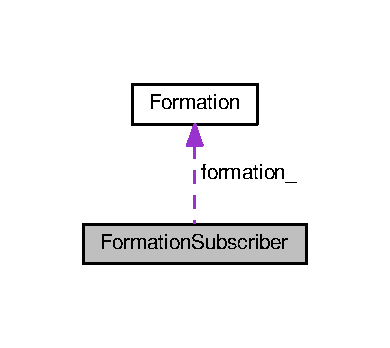
\includegraphics[width=187pt]{classFormationSubscriber__coll__graph}
\end{center}
\end{figure}
\subsection*{Public Member Functions}
\begin{DoxyCompactItemize}
\item 
{\bfseries Formation\+Subscriber} (ros\+::\+Node\+Handle \&nh, \hyperlink{classFormation}{Formation} $\ast$formation, std\+::vector$<$ std\+::string $>$ topics)\hypertarget{classFormationSubscriber_ab691695d88dd33de83c5a1a6688cc0df}{}\label{classFormationSubscriber_ab691695d88dd33de83c5a1a6688cc0df}

\item 
void {\bfseries callback\+\_\+odometry} (const nav\+\_\+msgs\+::\+Odometry\+Const\+Ptr \&msg, int number)\hypertarget{classFormationSubscriber_ad321467ea2f6538f7ee9c6fc233438d0}{}\label{classFormationSubscriber_ad321467ea2f6538f7ee9c6fc233438d0}

\item 
void {\bfseries callback\+\_\+laserscanner} (const sensor\+\_\+msgs\+::\+Laser\+Scan\+Const\+Ptr \&msg, int number)\hypertarget{classFormationSubscriber_a1eb720d4ce3016eb21cac0f33296eeae}{}\label{classFormationSubscriber_a1eb720d4ce3016eb21cac0f33296eeae}

\end{DoxyCompactItemize}
\subsection*{Private Attributes}
\begin{DoxyCompactItemize}
\item 
\hyperlink{classFormation}{Formation} $\ast$ {\bfseries formation\+\_\+}\hypertarget{classFormationSubscriber_a5c3e1951c929d9f8e069a6a3dfe617f7}{}\label{classFormationSubscriber_a5c3e1951c929d9f8e069a6a3dfe617f7}

\item 
tf\+::\+Transform\+Listener {\bfseries listener\+\_\+}\hypertarget{classFormationSubscriber_a73b853f947df83fd15788ee09729f5f2}{}\label{classFormationSubscriber_a73b853f947df83fd15788ee09729f5f2}

\item 
std\+::list$<$ ros\+::\+Subscriber $>$ {\bfseries odom\+\_\+subscribers\+\_\+}\hypertarget{classFormationSubscriber_ad9f976b3e787695511b231126b5690a9}{}\label{classFormationSubscriber_ad9f976b3e787695511b231126b5690a9}

\item 
std\+::list$<$ ros\+::\+Subscriber $>$ {\bfseries laser\+\_\+subscribers\+\_\+}\hypertarget{classFormationSubscriber_a07c4f6a377d998cf14fb152c155e0798}{}\label{classFormationSubscriber_a07c4f6a377d998cf14fb152c155e0798}

\end{DoxyCompactItemize}


The documentation for this class was generated from the following files\+:\begin{DoxyCompactItemize}
\item 
formation/include/formation/formation\+\_\+subscriber.\+h\item 
formation/src/formation\+\_\+subscriber.\+cpp\end{DoxyCompactItemize}

\hypertarget{structLaserPredictor_1_1Frames}{}\section{Laser\+Predictor\+:\+:Frames Struct Reference}
\label{structLaserPredictor_1_1Frames}\index{Laser\+Predictor\+::\+Frames@{Laser\+Predictor\+::\+Frames}}


Holds the names of all the necessary frames for the prediction class.  




{\ttfamily \#include $<$laser\+\_\+predictor.\+h$>$}

\subsection*{Public Member Functions}
\begin{DoxyCompactItemize}
\item 
\hyperlink{structLaserPredictor_1_1Frames_a9db5f1195d8982e3d63d981dafe517f4}{Frames} (std\+::string \hyperlink{structLaserPredictor_1_1Frames_a279efa689fc1b142d95055b8d85b0b3e}{base}, std\+::string \hyperlink{structLaserPredictor_1_1Frames_a204e91ead9b16ec6562746d13eb4828a}{front}, std\+::string \hyperlink{structLaserPredictor_1_1Frames_a28b95577e6a88d8211ddaa9f99fb90f4}{back})
\begin{DoxyCompactList}\small\item\em Construct a new \hyperlink{structLaserPredictor_1_1Frames}{Frames} object. \end{DoxyCompactList}\end{DoxyCompactItemize}
\subsection*{Public Attributes}
\begin{DoxyCompactItemize}
\item 
std\+::string \hyperlink{structLaserPredictor_1_1Frames_a279efa689fc1b142d95055b8d85b0b3e}{base}\hypertarget{structLaserPredictor_1_1Frames_a279efa689fc1b142d95055b8d85b0b3e}{}\label{structLaserPredictor_1_1Frames_a279efa689fc1b142d95055b8d85b0b3e}

\begin{DoxyCompactList}\small\item\em Frame name of base link. \end{DoxyCompactList}\item 
std\+::string \hyperlink{structLaserPredictor_1_1Frames_a204e91ead9b16ec6562746d13eb4828a}{front}\hypertarget{structLaserPredictor_1_1Frames_a204e91ead9b16ec6562746d13eb4828a}{}\label{structLaserPredictor_1_1Frames_a204e91ead9b16ec6562746d13eb4828a}

\begin{DoxyCompactList}\small\item\em Frame name of front laser link. \end{DoxyCompactList}\item 
std\+::string \hyperlink{structLaserPredictor_1_1Frames_a28b95577e6a88d8211ddaa9f99fb90f4}{back}\hypertarget{structLaserPredictor_1_1Frames_a28b95577e6a88d8211ddaa9f99fb90f4}{}\label{structLaserPredictor_1_1Frames_a28b95577e6a88d8211ddaa9f99fb90f4}

\begin{DoxyCompactList}\small\item\em Frame name of the back laser link. \end{DoxyCompactList}\end{DoxyCompactItemize}


\subsection{Detailed Description}
Holds the names of all the necessary frames for the prediction class. 

\subsection{Constructor \& Destructor Documentation}
\index{Laser\+Predictor\+::\+Frames@{Laser\+Predictor\+::\+Frames}!Frames@{Frames}}
\index{Frames@{Frames}!Laser\+Predictor\+::\+Frames@{Laser\+Predictor\+::\+Frames}}
\subsubsection[{\texorpdfstring{Frames(std\+::string base, std\+::string front, std\+::string back)}{Frames(std::string base, std::string front, std::string back)}}]{\setlength{\rightskip}{0pt plus 5cm}Laser\+Predictor\+::\+Frames\+::\+Frames (
\begin{DoxyParamCaption}
\item[{std\+::string}]{base, }
\item[{std\+::string}]{front, }
\item[{std\+::string}]{back}
\end{DoxyParamCaption}
)\hspace{0.3cm}{\ttfamily [inline]}}\hypertarget{structLaserPredictor_1_1Frames_a9db5f1195d8982e3d63d981dafe517f4}{}\label{structLaserPredictor_1_1Frames_a9db5f1195d8982e3d63d981dafe517f4}


Construct a new \hyperlink{structLaserPredictor_1_1Frames}{Frames} object. 


\begin{DoxyParams}{Parameters}
{\em base} & Name of the base link \\
\hline
{\em front} & Name of the front laser link \\
\hline
{\em back} & Name of the back laser link \\
\hline
\end{DoxyParams}


The documentation for this struct was generated from the following file\+:\begin{DoxyCompactItemize}
\item 
formation/include/formation/laser\+\_\+predictor.\+h\end{DoxyCompactItemize}

\hypertarget{classgazebo_1_1GazeboRosLinkAttacher}{}\section{gazebo\+:\+:Gazebo\+Ros\+Link\+Attacher Class Reference}
\label{classgazebo_1_1GazeboRosLinkAttacher}\index{gazebo\+::\+Gazebo\+Ros\+Link\+Attacher@{gazebo\+::\+Gazebo\+Ros\+Link\+Attacher}}


Inheritance diagram for gazebo\+:\+:Gazebo\+Ros\+Link\+Attacher\+:\nopagebreak
\begin{figure}[H]
\begin{center}
\leavevmode
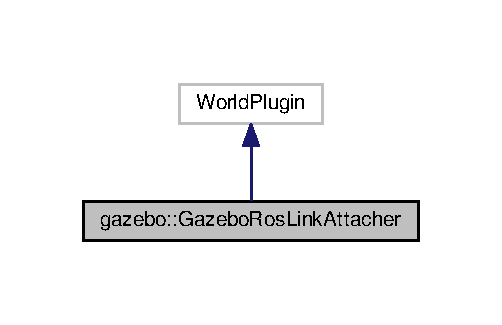
\includegraphics[width=241pt]{d9/d98/classgazebo_1_1GazeboRosLinkAttacher__inherit__graph}
\end{center}
\end{figure}


Collaboration diagram for gazebo\+:\+:Gazebo\+Ros\+Link\+Attacher\+:\nopagebreak
\begin{figure}[H]
\begin{center}
\leavevmode
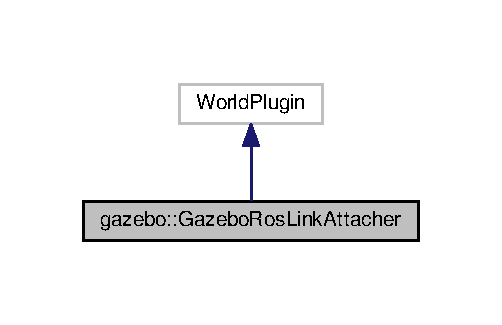
\includegraphics[width=241pt]{dc/da6/classgazebo_1_1GazeboRosLinkAttacher__coll__graph}
\end{center}
\end{figure}
\subsection*{Classes}
\begin{DoxyCompactItemize}
\item 
struct \hyperlink{structgazebo_1_1GazeboRosLinkAttacher_1_1fixedJoint}{fixed\+Joint}
\begin{DoxyCompactList}\small\item\em Internal representation of a fixed joint. \end{DoxyCompactList}\end{DoxyCompactItemize}
\subsection*{Public Member Functions}
\begin{DoxyCompactItemize}
\item 
\hyperlink{classgazebo_1_1GazeboRosLinkAttacher_a78371f65eeba823c1ba2d9afa1ec6947}{Gazebo\+Ros\+Link\+Attacher} ()\hypertarget{classgazebo_1_1GazeboRosLinkAttacher_a78371f65eeba823c1ba2d9afa1ec6947}{}\label{classgazebo_1_1GazeboRosLinkAttacher_a78371f65eeba823c1ba2d9afa1ec6947}

\begin{DoxyCompactList}\small\item\em Constructor. \end{DoxyCompactList}\item 
virtual \hyperlink{classgazebo_1_1GazeboRosLinkAttacher_a11bae998a168b982dbe92789904570db}{$\sim$\+Gazebo\+Ros\+Link\+Attacher} ()\hypertarget{classgazebo_1_1GazeboRosLinkAttacher_a11bae998a168b982dbe92789904570db}{}\label{classgazebo_1_1GazeboRosLinkAttacher_a11bae998a168b982dbe92789904570db}

\begin{DoxyCompactList}\small\item\em Destructor. \end{DoxyCompactList}\item 
void \hyperlink{classgazebo_1_1GazeboRosLinkAttacher_a11e7446b442f0cdbde9ca5d7947868c6}{Load} (physics\+::\+World\+Ptr \+\_\+world, sdf\+::\+Element\+Ptr)\hypertarget{classgazebo_1_1GazeboRosLinkAttacher_a11e7446b442f0cdbde9ca5d7947868c6}{}\label{classgazebo_1_1GazeboRosLinkAttacher_a11e7446b442f0cdbde9ca5d7947868c6}

\begin{DoxyCompactList}\small\item\em Load the controller. \end{DoxyCompactList}\item 
bool \hyperlink{classgazebo_1_1GazeboRosLinkAttacher_aa78798706ecdfe0dcbf905efbfc810fe}{attach} (std\+::string model1, std\+::string link1, std\+::string model2, std\+::string link2, std\+::string joint\+\_\+type)\hypertarget{classgazebo_1_1GazeboRosLinkAttacher_aa78798706ecdfe0dcbf905efbfc810fe}{}\label{classgazebo_1_1GazeboRosLinkAttacher_aa78798706ecdfe0dcbf905efbfc810fe}

\begin{DoxyCompactList}\small\item\em Attach with a revolute joint. \end{DoxyCompactList}\item 
bool \hyperlink{classgazebo_1_1GazeboRosLinkAttacher_a83db223615f28836f6f3cdc6590ed2c7}{detach} (std\+::string model1, std\+::string link1, std\+::string model2, std\+::string link2)\hypertarget{classgazebo_1_1GazeboRosLinkAttacher_a83db223615f28836f6f3cdc6590ed2c7}{}\label{classgazebo_1_1GazeboRosLinkAttacher_a83db223615f28836f6f3cdc6590ed2c7}

\begin{DoxyCompactList}\small\item\em Detach. \end{DoxyCompactList}\item 
bool {\bfseries get\+Joint} (std\+::string model1, std\+::string link1, std\+::string model2, std\+::string link2, \hyperlink{structgazebo_1_1GazeboRosLinkAttacher_1_1fixedJoint}{fixed\+Joint} \&joint)\hypertarget{classgazebo_1_1GazeboRosLinkAttacher_ac894e753858bc9037956bc164970dea1}{}\label{classgazebo_1_1GazeboRosLinkAttacher_ac894e753858bc9037956bc164970dea1}

\end{DoxyCompactItemize}
\subsection*{Private Member Functions}
\begin{DoxyCompactItemize}
\item 
bool {\bfseries attach\+\_\+callback} (gazebo\+\_\+ros\+\_\+link\+\_\+attacher\+::\+Attach\+::\+Request \&req, gazebo\+\_\+ros\+\_\+link\+\_\+attacher\+::\+Attach\+::\+Response \&res)\hypertarget{classgazebo_1_1GazeboRosLinkAttacher_a77b58d1c8f8f9887c4eacdbae33dbbc2}{}\label{classgazebo_1_1GazeboRosLinkAttacher_a77b58d1c8f8f9887c4eacdbae33dbbc2}

\item 
bool {\bfseries detach\+\_\+callback} (gazebo\+\_\+ros\+\_\+link\+\_\+attacher\+::\+Attach\+::\+Request \&req, gazebo\+\_\+ros\+\_\+link\+\_\+attacher\+::\+Attach\+::\+Response \&res)\hypertarget{classgazebo_1_1GazeboRosLinkAttacher_a63e93b7efb7c97e80bab07ea0a0a0fb6}{}\label{classgazebo_1_1GazeboRosLinkAttacher_a63e93b7efb7c97e80bab07ea0a0a0fb6}

\end{DoxyCompactItemize}
\subsection*{Private Attributes}
\begin{DoxyCompactItemize}
\item 
ros\+::\+Node\+Handle {\bfseries nh\+\_\+}\hypertarget{classgazebo_1_1GazeboRosLinkAttacher_aa9f2e548b0d54e7654f5d695465c35d8}{}\label{classgazebo_1_1GazeboRosLinkAttacher_aa9f2e548b0d54e7654f5d695465c35d8}

\item 
ros\+::\+Service\+Server {\bfseries attach\+\_\+service\+\_\+}\hypertarget{classgazebo_1_1GazeboRosLinkAttacher_a0ad42302b9f911db4c4ee4575da1b21b}{}\label{classgazebo_1_1GazeboRosLinkAttacher_a0ad42302b9f911db4c4ee4575da1b21b}

\item 
ros\+::\+Service\+Server {\bfseries detach\+\_\+service\+\_\+}\hypertarget{classgazebo_1_1GazeboRosLinkAttacher_ac367ec2e6d4586a0b0012691c1eb9b9e}{}\label{classgazebo_1_1GazeboRosLinkAttacher_ac367ec2e6d4586a0b0012691c1eb9b9e}

\item 
std\+::vector$<$ \hyperlink{structgazebo_1_1GazeboRosLinkAttacher_1_1fixedJoint}{fixed\+Joint} $>$ {\bfseries joints}\hypertarget{classgazebo_1_1GazeboRosLinkAttacher_a923603dd1f79d61db2eb00deab94b84f}{}\label{classgazebo_1_1GazeboRosLinkAttacher_a923603dd1f79d61db2eb00deab94b84f}

\item 
physics\+::\+Physics\+Engine\+Ptr \hyperlink{classgazebo_1_1GazeboRosLinkAttacher_a123418ffa0ed6705f100fe4c2ede7a03}{physics}\hypertarget{classgazebo_1_1GazeboRosLinkAttacher_a123418ffa0ed6705f100fe4c2ede7a03}{}\label{classgazebo_1_1GazeboRosLinkAttacher_a123418ffa0ed6705f100fe4c2ede7a03}

\begin{DoxyCompactList}\small\item\em The physics engine. \end{DoxyCompactList}\item 
physics\+::\+World\+Ptr \hyperlink{classgazebo_1_1GazeboRosLinkAttacher_a5f6e8a6b84a0f04ff9a39bf53ff651fe}{world}\hypertarget{classgazebo_1_1GazeboRosLinkAttacher_a5f6e8a6b84a0f04ff9a39bf53ff651fe}{}\label{classgazebo_1_1GazeboRosLinkAttacher_a5f6e8a6b84a0f04ff9a39bf53ff651fe}

\begin{DoxyCompactList}\small\item\em Pointer to the world. \end{DoxyCompactList}\end{DoxyCompactItemize}


The documentation for this class was generated from the following files\+:\begin{DoxyCompactItemize}
\item 
gazebo\+\_\+ros\+\_\+link\+\_\+attacher/include/gazebo\+\_\+ros\+\_\+link\+\_\+attacher.\+h\item 
gazebo\+\_\+ros\+\_\+link\+\_\+attacher/src/gazebo\+\_\+ros\+\_\+link\+\_\+attacher.\+cpp\end{DoxyCompactItemize}

\hypertarget{classLaserPredictor}{}\section{Laser\+Predictor Class Reference}
\label{classLaserPredictor}\index{Laser\+Predictor@{Laser\+Predictor}}


A class for predictings neighbour robots from the laser scanner data of another robot.  




{\ttfamily \#include $<$laser\+\_\+predictor.\+h$>$}



Collaboration diagram for Laser\+Predictor\+:\nopagebreak
\begin{figure}[H]
\begin{center}
\leavevmode
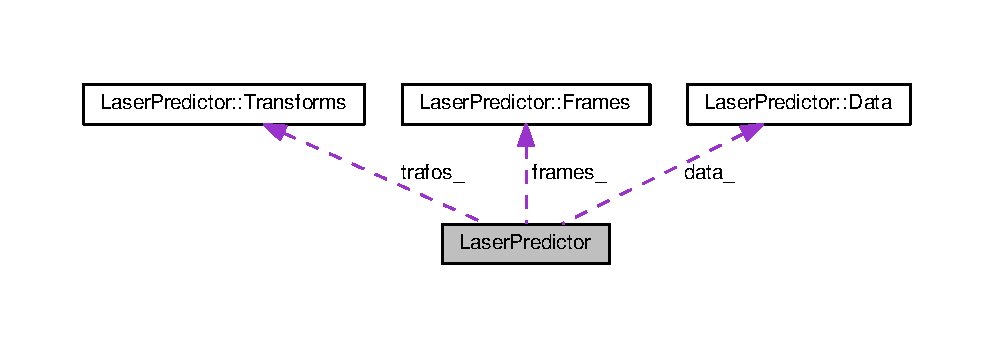
\includegraphics[width=350pt]{classLaserPredictor__coll__graph}
\end{center}
\end{figure}
\subsection*{Classes}
\begin{DoxyCompactItemize}
\item 
struct \hyperlink{structLaserPredictor_1_1Data}{Data}
\begin{DoxyCompactList}\small\item\em Holds all the data used within the predictor. \end{DoxyCompactList}\item 
struct \hyperlink{structLaserPredictor_1_1Frames}{Frames}
\begin{DoxyCompactList}\small\item\em Holds the names of all the necessary frames for the prediction class. \end{DoxyCompactList}\item 
struct \hyperlink{structLaserPredictor_1_1Transforms}{Transforms}
\begin{DoxyCompactList}\small\item\em Holds all necessary transformations. \end{DoxyCompactList}\end{DoxyCompactItemize}
\subsection*{Public Types}
\begin{DoxyCompactItemize}
\item 
typedef std\+::vector$<$ tf\+::\+Pose $>$ \hyperlink{classLaserPredictor_a6c7dc6bd4bfb6acd3d95e88e1b9b4be2}{Poses}\hypertarget{classLaserPredictor_a6c7dc6bd4bfb6acd3d95e88e1b9b4be2}{}\label{classLaserPredictor_a6c7dc6bd4bfb6acd3d95e88e1b9b4be2}

\begin{DoxyCompactList}\small\item\em Defines Poses as a std\+::vector of tf\+::\+Poses. \end{DoxyCompactList}\item 
typedef std\+::vector$<$ tf\+::\+Point $>$ \hyperlink{classLaserPredictor_ae2e95d6f06a21cf4a0b0bb0e369270b4}{Points}\hypertarget{classLaserPredictor_ae2e95d6f06a21cf4a0b0bb0e369270b4}{}\label{classLaserPredictor_ae2e95d6f06a21cf4a0b0bb0e369270b4}

\begin{DoxyCompactList}\small\item\em Defines Points as a std\+::vector of tf\+::\+Points. \end{DoxyCompactList}\item 
typedef sensor\+\_\+msgs\+::\+Point\+Cloud \hyperlink{classLaserPredictor_ae6d64da5bf82f544a2ea8a421af5a677}{Cloud}\hypertarget{classLaserPredictor_ae6d64da5bf82f544a2ea8a421af5a677}{}\label{classLaserPredictor_ae6d64da5bf82f544a2ea8a421af5a677}

\begin{DoxyCompactList}\small\item\em Defines Cloud as sensor\+\_\+msgs\+::\+Point\+Cloud. \end{DoxyCompactList}\item 
typedef \hyperlink{structLaserPredictor_1_1Frames}{Frames} \hyperlink{classLaserPredictor_a3d60b85935a522f854a8f0a34bb7b3ca}{Topics}\hypertarget{classLaserPredictor_a3d60b85935a522f854a8f0a34bb7b3ca}{}\label{classLaserPredictor_a3d60b85935a522f854a8f0a34bb7b3ca}

\begin{DoxyCompactList}\small\item\em Defines Topics as \hyperlink{structLaserPredictor_1_1Frames}{Frames}. Topics holds simmilare names as \hyperlink{structLaserPredictor_1_1Frames}{Frames} but for topics not for frames. \end{DoxyCompactList}\item 
typedef std\+::vector$<$ sensor\+\_\+msgs\+::\+Point\+Cloud $>$ \hyperlink{classLaserPredictor_ab05e971dfcde2d9abbabe861681a541c}{Clusters}\hypertarget{classLaserPredictor_ab05e971dfcde2d9abbabe861681a541c}{}\label{classLaserPredictor_ab05e971dfcde2d9abbabe861681a541c}

\begin{DoxyCompactList}\small\item\em Defines Clusters as vector of Point\+Clouds. \end{DoxyCompactList}\end{DoxyCompactItemize}
\subsection*{Public Member Functions}
\begin{DoxyCompactItemize}
\item 
\hyperlink{classLaserPredictor_a8a1c3d15f619d2b4114ffa2907cddbfb}{Laser\+Predictor} (ros\+::\+Node\+Handle \&nh, \hyperlink{structLaserPredictor_1_1Frames}{Frames} frames, \hyperlink{classLaserPredictor_a3d60b85935a522f854a8f0a34bb7b3ca}{Topics} topic)
\begin{DoxyCompactList}\small\item\em Construct a new Laser Predictor object. \end{DoxyCompactList}\item 
int \hyperlink{classLaserPredictor_a9634b4a17a0fbef515cd95c7aab5832f}{get\+Number\+Of\+Predictions} ()
\begin{DoxyCompactList}\small\item\em Get the Number Of Predictions object. \end{DoxyCompactList}\item 
\hyperlink{classLaserPredictor_a6c7dc6bd4bfb6acd3d95e88e1b9b4be2}{Poses} \hyperlink{classLaserPredictor_a91056be74cceed6f4fa79154118b69c0}{get\+Poses} ()
\begin{DoxyCompactList}\small\item\em Get the predicted Poses. \end{DoxyCompactList}\item 
tf\+::\+Pose \hyperlink{classLaserPredictor_a3d5fcd96bfdb75a0ad582b14ff2e04dd}{get\+Pose} (int i)
\begin{DoxyCompactList}\small\item\em Get one of the Pose objects. \end{DoxyCompactList}\item 
\hyperlink{classLaserPredictor_ae6d64da5bf82f544a2ea8a421af5a677}{Cloud} \hyperlink{classLaserPredictor_aafd0b92c01204d5b6ce494944e1ff381}{get\+Registered\+Points} ()
\begin{DoxyCompactList}\small\item\em Get the combination of front and back laser data. \end{DoxyCompactList}\item 
\hyperlink{classLaserPredictor_ae6d64da5bf82f544a2ea8a421af5a677}{Cloud} \hyperlink{classLaserPredictor_a665b9b39107726f46c5258908fc0abe4}{get\+Clustered\+Points} ()
\begin{DoxyCompactList}\small\item\em Get the combinaton of front and back laser data with cluster signature. \end{DoxyCompactList}\item 
void \hyperlink{classLaserPredictor_aa43afd04407b1a92d1ea722cc8d6d4bc}{guess} (\hyperlink{classLaserPredictor_a6c7dc6bd4bfb6acd3d95e88e1b9b4be2}{Poses} values)
\begin{DoxyCompactList}\small\item\em Give a guess where cluster(robots) are with respect to the base link frame. \end{DoxyCompactList}\item 
void \hyperlink{classLaserPredictor_a5e9c2c66bd54512e480bbc1c88d2c13d}{start\+Clustering} (double frequenzy)
\begin{DoxyCompactList}\small\item\em Starts the cluster algorithm. \end{DoxyCompactList}\end{DoxyCompactItemize}
\subsection*{Static Public Member Functions}
\begin{DoxyCompactItemize}
\item 
static \hyperlink{classLaserPredictor_ae6d64da5bf82f544a2ea8a421af5a677}{Cloud} \hyperlink{classLaserPredictor_a10a142e38f04a4459aa6d6783c87f1cd}{combine\+Data} (\hyperlink{classLaserPredictor_ae6d64da5bf82f544a2ea8a421af5a677}{Cloud} front, \hyperlink{classLaserPredictor_ae6d64da5bf82f544a2ea8a421af5a677}{Cloud} back)
\begin{DoxyCompactList}\small\item\em Combines the data front and back together. \end{DoxyCompactList}\item 
static void \hyperlink{classLaserPredictor_a06751e2996c1021bb8f4e4952b6286a4}{transform\+Cloud} (\hyperlink{classLaserPredictor_ae6d64da5bf82f544a2ea8a421af5a677}{Cloud} \&cloud, tf\+::\+Transform trafo)
\begin{DoxyCompactList}\small\item\em Applies the transform trafo to each point in the cloud. \end{DoxyCompactList}\end{DoxyCompactItemize}
\subsection*{Private Member Functions}
\begin{DoxyCompactItemize}
\item 
void \hyperlink{classLaserPredictor_a5f7f9dadce39c6060951ffefe590e834}{clustering} (const ros\+::\+Timer\+Event \&event)
\begin{DoxyCompactList}\small\item\em Timer callback to execute the cluster algorithm. \end{DoxyCompactList}\item 
\hyperlink{classLaserPredictor_ab05e971dfcde2d9abbabe861681a541c}{Clusters} \hyperlink{classLaserPredictor_aa1ba5f881fb2b50827bf6ef0802e596b}{k\+Means} (\hyperlink{classLaserPredictor_ae6d64da5bf82f544a2ea8a421af5a677}{Cloud} \&data, \hyperlink{classLaserPredictor_ae2e95d6f06a21cf4a0b0bb0e369270b4}{Points} \&centers)
\begin{DoxyCompactList}\small\item\em Executes k-\/means clustering at the data with respect to the guessed cluster ceneters centers. \end{DoxyCompactList}\item 
\hyperlink{classLaserPredictor_ab05e971dfcde2d9abbabe861681a541c}{Clusters} \hyperlink{classLaserPredictor_ab7fde5a32b1ac2dadc62aff4202a0456}{k\+Means} (\hyperlink{classLaserPredictor_ae6d64da5bf82f544a2ea8a421af5a677}{Cloud} \&data, \hyperlink{classLaserPredictor_a6c7dc6bd4bfb6acd3d95e88e1b9b4be2}{Poses} \&centers)
\begin{DoxyCompactList}\small\item\em Executes k-\/means clustering at the data with respect to the guessed cluster ceneters centers. \end{DoxyCompactList}\item 
void \hyperlink{classLaserPredictor_a58641b51a4d1120f6242b34def65d837}{subscriber\+Front\+Callback} (const sensor\+\_\+msgs\+::\+Laser\+Scan\+Const\+Ptr msg)
\begin{DoxyCompactList}\small\item\em Callback for the front laser scanner subscribtion. \end{DoxyCompactList}\item 
void \hyperlink{classLaserPredictor_a33365cf376510441f49e19588674ead2}{subscriber\+Back\+Callback} (const sensor\+\_\+msgs\+::\+Laser\+Scan\+Const\+Ptr msg)
\begin{DoxyCompactList}\small\item\em Callback for the back laser scanner subscribtion. \end{DoxyCompactList}\end{DoxyCompactItemize}
\subsection*{Private Attributes}
\begin{DoxyCompactItemize}
\item 
ros\+::\+Node\+Handle \hyperlink{classLaserPredictor_a9535842866b44234078f0f69bbeb8539}{nh\+\_\+}\hypertarget{classLaserPredictor_a9535842866b44234078f0f69bbeb8539}{}\label{classLaserPredictor_a9535842866b44234078f0f69bbeb8539}

\begin{DoxyCompactList}\small\item\em Nodehandle for handling namespaces and ros functionality. \end{DoxyCompactList}\item 
ros\+::\+Subscriber \hyperlink{classLaserPredictor_a0cce21a3c340df330f68c4bdc91562f8}{sub\+\_\+front\+\_\+}\hypertarget{classLaserPredictor_a0cce21a3c340df330f68c4bdc91562f8}{}\label{classLaserPredictor_a0cce21a3c340df330f68c4bdc91562f8}

\begin{DoxyCompactList}\small\item\em Subscriber for front laser scanner. \end{DoxyCompactList}\item 
ros\+::\+Subscriber \hyperlink{classLaserPredictor_a3ba0934ebaf60999f241314955038fbf}{sub\+\_\+back\+\_\+}\hypertarget{classLaserPredictor_a3ba0934ebaf60999f241314955038fbf}{}\label{classLaserPredictor_a3ba0934ebaf60999f241314955038fbf}

\begin{DoxyCompactList}\small\item\em Subscriber for back laser scanner. \end{DoxyCompactList}\item 
ros\+::\+Timer \hyperlink{classLaserPredictor_a304d7c60e689819cc6e6398bee80a891}{cluster\+\_\+scope\+\_\+}\hypertarget{classLaserPredictor_a304d7c60e689819cc6e6398bee80a891}{}\label{classLaserPredictor_a304d7c60e689819cc6e6398bee80a891}

\begin{DoxyCompactList}\small\item\em Timer for the clustering scope. \end{DoxyCompactList}\item 
laser\+\_\+geometry\+::\+Laser\+Projection \hyperlink{classLaserPredictor_a02d304374282c92530ffce61fa31dc31}{projector\+\_\+}\hypertarget{classLaserPredictor_a02d304374282c92530ffce61fa31dc31}{}\label{classLaserPredictor_a02d304374282c92530ffce61fa31dc31}

\begin{DoxyCompactList}\small\item\em Is yoused to project the laser scanner data into cartesian space. \end{DoxyCompactList}\item 
\hyperlink{structLaserPredictor_1_1Transforms}{Transforms} \hyperlink{classLaserPredictor_a462937a6b7f66cb731f53659fa69c215}{trafos\+\_\+}\hypertarget{classLaserPredictor_a462937a6b7f66cb731f53659fa69c215}{}\label{classLaserPredictor_a462937a6b7f66cb731f53659fa69c215}

\begin{DoxyCompactList}\small\item\em Holds the trasnformatiosn from base to the laser links. \end{DoxyCompactList}\item 
\hyperlink{structLaserPredictor_1_1Frames}{Frames} \hyperlink{classLaserPredictor_a381370876c2606b7aa690959490237f9}{frames\+\_\+}\hypertarget{classLaserPredictor_a381370876c2606b7aa690959490237f9}{}\label{classLaserPredictor_a381370876c2606b7aa690959490237f9}

\begin{DoxyCompactList}\small\item\em Holds the names of the links of the base and the laser links. \end{DoxyCompactList}\item 
\hyperlink{structLaserPredictor_1_1Data}{Data} \hyperlink{classLaserPredictor_a897df6d3a3d9a810ef7b586f83415046}{data\+\_\+}\hypertarget{classLaserPredictor_a897df6d3a3d9a810ef7b586f83415046}{}\label{classLaserPredictor_a897df6d3a3d9a810ef7b586f83415046}

\begin{DoxyCompactList}\small\item\em Holds all pointcloud data. \end{DoxyCompactList}\item 
\hyperlink{classLaserPredictor_a6c7dc6bd4bfb6acd3d95e88e1b9b4be2}{Poses} \hyperlink{classLaserPredictor_a0cffbd5cd61e29cd1e137854935d0072}{poses\+\_\+}\hypertarget{classLaserPredictor_a0cffbd5cd61e29cd1e137854935d0072}{}\label{classLaserPredictor_a0cffbd5cd61e29cd1e137854935d0072}

\begin{DoxyCompactList}\small\item\em Holds all estaminated poses of the robots. \end{DoxyCompactList}\end{DoxyCompactItemize}


\subsection{Detailed Description}
A class for predictings neighbour robots from the laser scanner data of another robot. 

\subsection{Constructor \& Destructor Documentation}
\index{Laser\+Predictor@{Laser\+Predictor}!Laser\+Predictor@{Laser\+Predictor}}
\index{Laser\+Predictor@{Laser\+Predictor}!Laser\+Predictor@{Laser\+Predictor}}
\subsubsection[{\texorpdfstring{Laser\+Predictor(ros\+::\+Node\+Handle \&nh, Frames frames, Topics topic)}{LaserPredictor(ros::NodeHandle &nh, Frames frames, Topics topic)}}]{\setlength{\rightskip}{0pt plus 5cm}Laser\+Predictor\+::\+Laser\+Predictor (
\begin{DoxyParamCaption}
\item[{ros\+::\+Node\+Handle \&}]{nh, }
\item[{{\bf Frames}}]{frames, }
\item[{{\bf Topics}}]{topic}
\end{DoxyParamCaption}
)}\hypertarget{classLaserPredictor_a8a1c3d15f619d2b4114ffa2907cddbfb}{}\label{classLaserPredictor_a8a1c3d15f619d2b4114ffa2907cddbfb}


Construct a new Laser Predictor object. 


\begin{DoxyParams}{Parameters}
{\em nh} & Node handle to handle namespaces and ros fucntionality \\
\hline
{\em frames} & Holds all the nescessary frames for the predictor \\
\hline
{\em topic} & Holds all the nescessary topics for the predictor \\
\hline
\end{DoxyParams}


\subsection{Member Function Documentation}
\index{Laser\+Predictor@{Laser\+Predictor}!clustering@{clustering}}
\index{clustering@{clustering}!Laser\+Predictor@{Laser\+Predictor}}
\subsubsection[{\texorpdfstring{clustering(const ros\+::\+Timer\+Event \&event)}{clustering(const ros::TimerEvent &event)}}]{\setlength{\rightskip}{0pt plus 5cm}void Laser\+Predictor\+::clustering (
\begin{DoxyParamCaption}
\item[{const ros\+::\+Timer\+Event \&}]{event}
\end{DoxyParamCaption}
)\hspace{0.3cm}{\ttfamily [private]}}\hypertarget{classLaserPredictor_a5f7f9dadce39c6060951ffefe590e834}{}\label{classLaserPredictor_a5f7f9dadce39c6060951ffefe590e834}


Timer callback to execute the cluster algorithm. 


\begin{DoxyParams}{Parameters}
{\em event} & Ros timer event \\
\hline
\end{DoxyParams}
\index{Laser\+Predictor@{Laser\+Predictor}!combine\+Data@{combine\+Data}}
\index{combine\+Data@{combine\+Data}!Laser\+Predictor@{Laser\+Predictor}}
\subsubsection[{\texorpdfstring{combine\+Data(\+Cloud front, Cloud back)}{combineData(Cloud front, Cloud back)}}]{\setlength{\rightskip}{0pt plus 5cm}sensor\+\_\+msgs\+::\+Point\+Cloud Laser\+Predictor\+::combine\+Data (
\begin{DoxyParamCaption}
\item[{{\bf Cloud}}]{front, }
\item[{{\bf Cloud}}]{back}
\end{DoxyParamCaption}
)\hspace{0.3cm}{\ttfamily [static]}}\hypertarget{classLaserPredictor_a10a142e38f04a4459aa6d6783c87f1cd}{}\label{classLaserPredictor_a10a142e38f04a4459aa6d6783c87f1cd}


Combines the data front and back together. 


\begin{DoxyParams}{Parameters}
{\em front} & First Cloud to combine \\
\hline
{\em back} & Second Cloud to combine \\
\hline
\end{DoxyParams}
\begin{DoxyReturn}{Returns}
Cloud Combined cloud 
\end{DoxyReturn}
\index{Laser\+Predictor@{Laser\+Predictor}!get\+Clustered\+Points@{get\+Clustered\+Points}}
\index{get\+Clustered\+Points@{get\+Clustered\+Points}!Laser\+Predictor@{Laser\+Predictor}}
\subsubsection[{\texorpdfstring{get\+Clustered\+Points()}{getClusteredPoints()}}]{\setlength{\rightskip}{0pt plus 5cm}sensor\+\_\+msgs\+::\+Point\+Cloud Laser\+Predictor\+::get\+Clustered\+Points (
\begin{DoxyParamCaption}
{}
\end{DoxyParamCaption}
)}\hypertarget{classLaserPredictor_a665b9b39107726f46c5258908fc0abe4}{}\label{classLaserPredictor_a665b9b39107726f46c5258908fc0abe4}


Get the combinaton of front and back laser data with cluster signature. 

\begin{DoxyReturn}{Returns}
Cloud \hyperlink{structLaserPredictor_1_1Data}{Data} wich holds a channel for the cluster number 
\end{DoxyReturn}
\index{Laser\+Predictor@{Laser\+Predictor}!get\+Number\+Of\+Predictions@{get\+Number\+Of\+Predictions}}
\index{get\+Number\+Of\+Predictions@{get\+Number\+Of\+Predictions}!Laser\+Predictor@{Laser\+Predictor}}
\subsubsection[{\texorpdfstring{get\+Number\+Of\+Predictions()}{getNumberOfPredictions()}}]{\setlength{\rightskip}{0pt plus 5cm}int Laser\+Predictor\+::get\+Number\+Of\+Predictions (
\begin{DoxyParamCaption}
{}
\end{DoxyParamCaption}
)}\hypertarget{classLaserPredictor_a9634b4a17a0fbef515cd95c7aab5832f}{}\label{classLaserPredictor_a9634b4a17a0fbef515cd95c7aab5832f}


Get the Number Of Predictions object. 

\begin{DoxyReturn}{Returns}
int Number of Predictions 
\end{DoxyReturn}
\index{Laser\+Predictor@{Laser\+Predictor}!get\+Pose@{get\+Pose}}
\index{get\+Pose@{get\+Pose}!Laser\+Predictor@{Laser\+Predictor}}
\subsubsection[{\texorpdfstring{get\+Pose(int i)}{getPose(int i)}}]{\setlength{\rightskip}{0pt plus 5cm}tf\+::\+Pose Laser\+Predictor\+::get\+Pose (
\begin{DoxyParamCaption}
\item[{int}]{i}
\end{DoxyParamCaption}
)}\hypertarget{classLaserPredictor_a3d5fcd96bfdb75a0ad582b14ff2e04dd}{}\label{classLaserPredictor_a3d5fcd96bfdb75a0ad582b14ff2e04dd}


Get one of the Pose objects. 


\begin{DoxyParams}{Parameters}
{\em i} & Index of the Pose to get \\
\hline
\end{DoxyParams}
\begin{DoxyReturn}{Returns}
tf\+::\+Pose Pose at this index 
\end{DoxyReturn}
\index{Laser\+Predictor@{Laser\+Predictor}!get\+Poses@{get\+Poses}}
\index{get\+Poses@{get\+Poses}!Laser\+Predictor@{Laser\+Predictor}}
\subsubsection[{\texorpdfstring{get\+Poses()}{getPoses()}}]{\setlength{\rightskip}{0pt plus 5cm}{\bf Laser\+Predictor\+::\+Poses} Laser\+Predictor\+::get\+Poses (
\begin{DoxyParamCaption}
{}
\end{DoxyParamCaption}
)}\hypertarget{classLaserPredictor_a91056be74cceed6f4fa79154118b69c0}{}\label{classLaserPredictor_a91056be74cceed6f4fa79154118b69c0}


Get the predicted Poses. 

\begin{DoxyReturn}{Returns}
Poses Predicted Poses 
\end{DoxyReturn}
\index{Laser\+Predictor@{Laser\+Predictor}!get\+Registered\+Points@{get\+Registered\+Points}}
\index{get\+Registered\+Points@{get\+Registered\+Points}!Laser\+Predictor@{Laser\+Predictor}}
\subsubsection[{\texorpdfstring{get\+Registered\+Points()}{getRegisteredPoints()}}]{\setlength{\rightskip}{0pt plus 5cm}sensor\+\_\+msgs\+::\+Point\+Cloud Laser\+Predictor\+::get\+Registered\+Points (
\begin{DoxyParamCaption}
{}
\end{DoxyParamCaption}
)}\hypertarget{classLaserPredictor_aafd0b92c01204d5b6ce494944e1ff381}{}\label{classLaserPredictor_aafd0b92c01204d5b6ce494944e1ff381}


Get the combination of front and back laser data. 

\begin{DoxyReturn}{Returns}
Cloud The combination of front and back laser data 
\end{DoxyReturn}
\index{Laser\+Predictor@{Laser\+Predictor}!guess@{guess}}
\index{guess@{guess}!Laser\+Predictor@{Laser\+Predictor}}
\subsubsection[{\texorpdfstring{guess(\+Poses values)}{guess(Poses values)}}]{\setlength{\rightskip}{0pt plus 5cm}void Laser\+Predictor\+::guess (
\begin{DoxyParamCaption}
\item[{{\bf Poses}}]{values}
\end{DoxyParamCaption}
)}\hypertarget{classLaserPredictor_aa43afd04407b1a92d1ea722cc8d6d4bc}{}\label{classLaserPredictor_aa43afd04407b1a92d1ea722cc8d6d4bc}


Give a guess where cluster(robots) are with respect to the base link frame. 


\begin{DoxyParams}{Parameters}
{\em values} & each tf\+::\+Pose specifies a possible robot and is used as start value for clustering algorithms \\
\hline
\end{DoxyParams}
\index{Laser\+Predictor@{Laser\+Predictor}!k\+Means@{k\+Means}}
\index{k\+Means@{k\+Means}!Laser\+Predictor@{Laser\+Predictor}}
\subsubsection[{\texorpdfstring{k\+Means(\+Cloud \&data, Points \&centers)}{kMeans(Cloud &data, Points &centers)}}]{\setlength{\rightskip}{0pt plus 5cm}{\bf Laser\+Predictor\+::\+Clusters} Laser\+Predictor\+::k\+Means (
\begin{DoxyParamCaption}
\item[{{\bf Cloud} \&}]{data, }
\item[{{\bf Points} \&}]{centers}
\end{DoxyParamCaption}
)\hspace{0.3cm}{\ttfamily [private]}}\hypertarget{classLaserPredictor_aa1ba5f881fb2b50827bf6ef0802e596b}{}\label{classLaserPredictor_aa1ba5f881fb2b50827bf6ef0802e596b}


Executes k-\/means clustering at the data with respect to the guessed cluster ceneters centers. 


\begin{DoxyParams}{Parameters}
{\em data} & \hyperlink{structLaserPredictor_1_1Data}{Data} wich are modified during the clustering process \\
\hline
{\em centers} & Centers wich are modified during the clustering process \\
\hline
\end{DoxyParams}
\begin{DoxyReturn}{Returns}
Points Final cluster centers 
\end{DoxyReturn}
\index{Laser\+Predictor@{Laser\+Predictor}!k\+Means@{k\+Means}}
\index{k\+Means@{k\+Means}!Laser\+Predictor@{Laser\+Predictor}}
\subsubsection[{\texorpdfstring{k\+Means(\+Cloud \&data, Poses \&centers)}{kMeans(Cloud &data, Poses &centers)}}]{\setlength{\rightskip}{0pt plus 5cm}{\bf Laser\+Predictor\+::\+Clusters} Laser\+Predictor\+::k\+Means (
\begin{DoxyParamCaption}
\item[{{\bf Cloud} \&}]{data, }
\item[{{\bf Poses} \&}]{centers}
\end{DoxyParamCaption}
)\hspace{0.3cm}{\ttfamily [private]}}\hypertarget{classLaserPredictor_ab7fde5a32b1ac2dadc62aff4202a0456}{}\label{classLaserPredictor_ab7fde5a32b1ac2dadc62aff4202a0456}


Executes k-\/means clustering at the data with respect to the guessed cluster ceneters centers. 


\begin{DoxyParams}{Parameters}
{\em data} & \hyperlink{structLaserPredictor_1_1Data}{Data} wich are modified during the clustering process \\
\hline
{\em centers} & Centers wich are modified during the clustering process \\
\hline
\end{DoxyParams}
\begin{DoxyReturn}{Returns}
Points Final cluster centers 
\end{DoxyReturn}
\index{Laser\+Predictor@{Laser\+Predictor}!start\+Clustering@{start\+Clustering}}
\index{start\+Clustering@{start\+Clustering}!Laser\+Predictor@{Laser\+Predictor}}
\subsubsection[{\texorpdfstring{start\+Clustering(double frequenzy)}{startClustering(double frequenzy)}}]{\setlength{\rightskip}{0pt plus 5cm}void Laser\+Predictor\+::start\+Clustering (
\begin{DoxyParamCaption}
\item[{double}]{frequenzy}
\end{DoxyParamCaption}
)}\hypertarget{classLaserPredictor_a5e9c2c66bd54512e480bbc1c88d2c13d}{}\label{classLaserPredictor_a5e9c2c66bd54512e480bbc1c88d2c13d}


Starts the cluster algorithm. 


\begin{DoxyParams}{Parameters}
{\em frequenzy} & Frequenzy how often the algorithm should be executed \\
\hline
\end{DoxyParams}
\index{Laser\+Predictor@{Laser\+Predictor}!subscriber\+Back\+Callback@{subscriber\+Back\+Callback}}
\index{subscriber\+Back\+Callback@{subscriber\+Back\+Callback}!Laser\+Predictor@{Laser\+Predictor}}
\subsubsection[{\texorpdfstring{subscriber\+Back\+Callback(const sensor\+\_\+msgs\+::\+Laser\+Scan\+Const\+Ptr msg)}{subscriberBackCallback(const sensor_msgs::LaserScanConstPtr msg)}}]{\setlength{\rightskip}{0pt plus 5cm}void Laser\+Predictor\+::subscriber\+Back\+Callback (
\begin{DoxyParamCaption}
\item[{const sensor\+\_\+msgs\+::\+Laser\+Scan\+Const\+Ptr}]{msg}
\end{DoxyParamCaption}
)\hspace{0.3cm}{\ttfamily [private]}}\hypertarget{classLaserPredictor_a33365cf376510441f49e19588674ead2}{}\label{classLaserPredictor_a33365cf376510441f49e19588674ead2}


Callback for the back laser scanner subscribtion. 


\begin{DoxyParams}{Parameters}
{\em msg} & data at the laser scanner topic \\
\hline
\end{DoxyParams}
\index{Laser\+Predictor@{Laser\+Predictor}!subscriber\+Front\+Callback@{subscriber\+Front\+Callback}}
\index{subscriber\+Front\+Callback@{subscriber\+Front\+Callback}!Laser\+Predictor@{Laser\+Predictor}}
\subsubsection[{\texorpdfstring{subscriber\+Front\+Callback(const sensor\+\_\+msgs\+::\+Laser\+Scan\+Const\+Ptr msg)}{subscriberFrontCallback(const sensor_msgs::LaserScanConstPtr msg)}}]{\setlength{\rightskip}{0pt plus 5cm}void Laser\+Predictor\+::subscriber\+Front\+Callback (
\begin{DoxyParamCaption}
\item[{const sensor\+\_\+msgs\+::\+Laser\+Scan\+Const\+Ptr}]{msg}
\end{DoxyParamCaption}
)\hspace{0.3cm}{\ttfamily [private]}}\hypertarget{classLaserPredictor_a58641b51a4d1120f6242b34def65d837}{}\label{classLaserPredictor_a58641b51a4d1120f6242b34def65d837}


Callback for the front laser scanner subscribtion. 


\begin{DoxyParams}{Parameters}
{\em msg} & data at the laser scanner topic \\
\hline
\end{DoxyParams}
\index{Laser\+Predictor@{Laser\+Predictor}!transform\+Cloud@{transform\+Cloud}}
\index{transform\+Cloud@{transform\+Cloud}!Laser\+Predictor@{Laser\+Predictor}}
\subsubsection[{\texorpdfstring{transform\+Cloud(\+Cloud \&cloud, tf\+::\+Transform trafo)}{transformCloud(Cloud &cloud, tf::Transform trafo)}}]{\setlength{\rightskip}{0pt plus 5cm}void Laser\+Predictor\+::transform\+Cloud (
\begin{DoxyParamCaption}
\item[{{\bf Cloud} \&}]{cloud, }
\item[{tf\+::\+Transform}]{trafo}
\end{DoxyParamCaption}
)\hspace{0.3cm}{\ttfamily [static]}}\hypertarget{classLaserPredictor_a06751e2996c1021bb8f4e4952b6286a4}{}\label{classLaserPredictor_a06751e2996c1021bb8f4e4952b6286a4}


Applies the transform trafo to each point in the cloud. 


\begin{DoxyParams}{Parameters}
{\em cloud} & cloud to be transformed \\
\hline
{\em trafo} & trafo to be applied \\
\hline
\end{DoxyParams}


The documentation for this class was generated from the following files\+:\begin{DoxyCompactItemize}
\item 
formation/include/formation/laser\+\_\+predictor.\+h\item 
formation/src/laser\+\_\+predictor.\+cpp\end{DoxyCompactItemize}

\hypertarget{structLissajousPlanner_1_1LissajousPlan}{}\section{Lissajous\+Planner\+:\+:Lissajous\+Plan Struct Reference}
\label{structLissajousPlanner_1_1LissajousPlan}\index{Lissajous\+Planner\+::\+Lissajous\+Plan@{Lissajous\+Planner\+::\+Lissajous\+Plan}}
\subsection*{Public Attributes}
\begin{DoxyCompactItemize}
\item 
float {\bfseries dphi}\hypertarget{structLissajousPlanner_1_1LissajousPlan_a60c6081d5506c1be5e0c4b48d5980b8d}{}\label{structLissajousPlanner_1_1LissajousPlan_a60c6081d5506c1be5e0c4b48d5980b8d}

\item 
float {\bfseries omegax}\hypertarget{structLissajousPlanner_1_1LissajousPlan_a54e05e3d4666b9843c13afe751d868e6}{}\label{structLissajousPlanner_1_1LissajousPlan_a54e05e3d4666b9843c13afe751d868e6}

\item 
int {\bfseries ratio}\hypertarget{structLissajousPlanner_1_1LissajousPlan_a1d7a8cb09570d913576d0b3592674e1f}{}\label{structLissajousPlanner_1_1LissajousPlan_a1d7a8cb09570d913576d0b3592674e1f}

\item 
float {\bfseries Ax}\hypertarget{structLissajousPlanner_1_1LissajousPlan_a85bedcfba3d78cb16bd67cc402b674ef}{}\label{structLissajousPlanner_1_1LissajousPlan_a85bedcfba3d78cb16bd67cc402b674ef}

\item 
float {\bfseries Ay}\hypertarget{structLissajousPlanner_1_1LissajousPlan_a72082318cebb55674e68a3383a81721f}{}\label{structLissajousPlanner_1_1LissajousPlan_a72082318cebb55674e68a3383a81721f}

\end{DoxyCompactItemize}


The documentation for this struct was generated from the following file\+:\begin{DoxyCompactItemize}
\item 
simulation\+\_\+env/include/simulation\+\_\+env/planner.\+h\end{DoxyCompactItemize}

\hypertarget{classLissajousPlanner}{}\section{Lissajous\+Planner Class Reference}
\label{classLissajousPlanner}\index{Lissajous\+Planner@{Lissajous\+Planner}}


Inheritance diagram for Lissajous\+Planner\+:\nopagebreak
\begin{figure}[H]
\begin{center}
\leavevmode
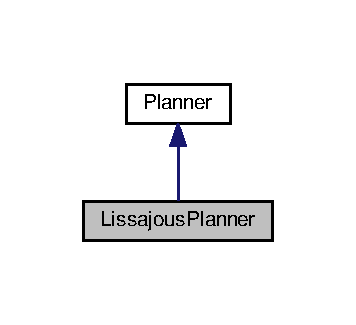
\includegraphics[width=171pt]{classLissajousPlanner__inherit__graph}
\end{center}
\end{figure}


Collaboration diagram for Lissajous\+Planner\+:\nopagebreak
\begin{figure}[H]
\begin{center}
\leavevmode
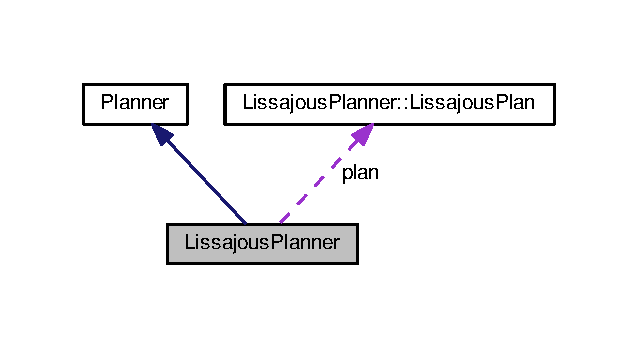
\includegraphics[width=306pt]{classLissajousPlanner__coll__graph}
\end{center}
\end{figure}
\subsection*{Classes}
\begin{DoxyCompactItemize}
\item 
struct \hyperlink{structLissajousPlanner_1_1LissajousPlan}{Lissajous\+Plan}
\end{DoxyCompactItemize}
\subsection*{Public Member Functions}
\begin{DoxyCompactItemize}
\item 
{\bfseries Lissajous\+Planner} (ros\+::\+Node\+Handle \&\hyperlink{classPlanner_a9714d036f444a07ce90be8d135b9a40c}{nh})\hypertarget{classLissajousPlanner_a82095ebb2cd29944a201321377fc78fe}{}\label{classLissajousPlanner_a82095ebb2cd29944a201321377fc78fe}

\item 
void {\bfseries set\+\_\+parameter} (float omegax, float dphi=0.\+0, int ratio=2, float Ax=3.\+0, float Ay=3.\+0)\hypertarget{classLissajousPlanner_aa6e4d941a535dca182aaf8b73b5a0dcd}{}\label{classLissajousPlanner_aa6e4d941a535dca182aaf8b73b5a0dcd}

\item 
void {\bfseries load} ()\hypertarget{classLissajousPlanner_ae7ecff9989a37d29e591bac082b781ac}{}\label{classLissajousPlanner_ae7ecff9989a37d29e591bac082b781ac}

\end{DoxyCompactItemize}
\subsection*{Private Member Functions}
\begin{DoxyCompactItemize}
\item 
tf\+::\+Vector3 {\bfseries get\+\_\+position} (ros\+::\+Duration time)\hypertarget{classLissajousPlanner_aeb9a2e0f3cb8e651518bcd0dcd80bf2f}{}\label{classLissajousPlanner_aeb9a2e0f3cb8e651518bcd0dcd80bf2f}

\item 
tf\+::\+Quaternion {\bfseries get\+\_\+orientation} (ros\+::\+Duration time)\hypertarget{classLissajousPlanner_a07eb5dc306609dd6ae1f91e2738aee95}{}\label{classLissajousPlanner_a07eb5dc306609dd6ae1f91e2738aee95}

\item 
tf\+::\+Vector3 {\bfseries get\+\_\+velocity} (ros\+::\+Duration time)\hypertarget{classLissajousPlanner_a17a85db0fe0f380164297b8365232ab2}{}\label{classLissajousPlanner_a17a85db0fe0f380164297b8365232ab2}

\item 
double {\bfseries get\+\_\+angular\+\_\+velocity} (ros\+::\+Duration time)\hypertarget{classLissajousPlanner_ab7ef88484995f3fd223c8dcbd6f86a8e}{}\label{classLissajousPlanner_ab7ef88484995f3fd223c8dcbd6f86a8e}

\item 
void {\bfseries check\+\_\+period} (ros\+::\+Duration time)\hypertarget{classLissajousPlanner_a9001fcfa7f1d25e4ae7826499b0b2ebc}{}\label{classLissajousPlanner_a9001fcfa7f1d25e4ae7826499b0b2ebc}

\end{DoxyCompactItemize}
\subsection*{Private Attributes}
\begin{DoxyCompactItemize}
\item 
\hyperlink{structLissajousPlanner_1_1LissajousPlan}{Lissajous\+Plan} {\bfseries plan}\hypertarget{classLissajousPlanner_ac3365f9d9d84307b680a94cff01edd9b}{}\label{classLissajousPlanner_ac3365f9d9d84307b680a94cff01edd9b}

\end{DoxyCompactItemize}
\subsection*{Additional Inherited Members}


The documentation for this class was generated from the following files\+:\begin{DoxyCompactItemize}
\item 
simulation\+\_\+env/include/simulation\+\_\+env/planner.\+h\item 
simulation\+\_\+env/src/planner.\+cpp\end{DoxyCompactItemize}

\hypertarget{structController_1_1LyapunovParameter}{}\section{Controller\+:\+:Lyapunov\+Parameter Struct Reference}
\label{structController_1_1LyapunovParameter}\index{Controller\+::\+Lyapunov\+Parameter@{Controller\+::\+Lyapunov\+Parameter}}


Specifies the parameters needed for the lyapunov based control law.  




{\ttfamily \#include $<$controller.\+h$>$}

\subsection*{Public Member Functions}
\begin{DoxyCompactItemize}
\item 
\hyperlink{structController_1_1LyapunovParameter_ae0d081687dfc7637bfbce3fe4cc2d9dd}{Lyapunov\+Parameter} ()\hypertarget{structController_1_1LyapunovParameter_ae0d081687dfc7637bfbce3fe4cc2d9dd}{}\label{structController_1_1LyapunovParameter_ae0d081687dfc7637bfbce3fe4cc2d9dd}

\begin{DoxyCompactList}\small\item\em Construct a new Lyapunov Parameter object with default Parameter. \end{DoxyCompactList}\item 
\hyperlink{structController_1_1LyapunovParameter_acca8d24226201cd98caa44ccd4ddc4ac}{Lyapunov\+Parameter} (float \hyperlink{structController_1_1LyapunovParameter_a4183bf21c97669dc44d4f67cb9a0d26c}{kx}, float \hyperlink{structController_1_1LyapunovParameter_a4cde698202cddb2fb3971fcc0f0804ca}{ky}, float \hyperlink{structController_1_1LyapunovParameter_a4ffd5e85451097367940acc6536d2a4c}{kphi})
\begin{DoxyCompactList}\small\item\em Construct a new Lyapunov Parameter object with given parameters. \end{DoxyCompactList}\item 
\hyperlink{structController_1_1LyapunovParameter_a5c8cfc9a6c9168848ddce0d15f17ec02}{Lyapunov\+Parameter} (std\+::vector$<$ float $>$ param)
\begin{DoxyCompactList}\small\item\em Construct a new Lyapunov Parameter object with given parameters by vector. \end{DoxyCompactList}\end{DoxyCompactItemize}
\subsection*{Public Attributes}
\begin{DoxyCompactItemize}
\item 
float \hyperlink{structController_1_1LyapunovParameter_a4183bf21c97669dc44d4f67cb9a0d26c}{kx}\hypertarget{structController_1_1LyapunovParameter_a4183bf21c97669dc44d4f67cb9a0d26c}{}\label{structController_1_1LyapunovParameter_a4183bf21c97669dc44d4f67cb9a0d26c}

\begin{DoxyCompactList}\small\item\em Control gain in x-\/direction. \end{DoxyCompactList}\item 
float \hyperlink{structController_1_1LyapunovParameter_a4cde698202cddb2fb3971fcc0f0804ca}{ky}\hypertarget{structController_1_1LyapunovParameter_a4cde698202cddb2fb3971fcc0f0804ca}{}\label{structController_1_1LyapunovParameter_a4cde698202cddb2fb3971fcc0f0804ca}

\begin{DoxyCompactList}\small\item\em Control gain in y-\/direction. \end{DoxyCompactList}\item 
float \hyperlink{structController_1_1LyapunovParameter_a4ffd5e85451097367940acc6536d2a4c}{kphi}\hypertarget{structController_1_1LyapunovParameter_a4ffd5e85451097367940acc6536d2a4c}{}\label{structController_1_1LyapunovParameter_a4ffd5e85451097367940acc6536d2a4c}

\begin{DoxyCompactList}\small\item\em Control gain in theta-\/direction. \end{DoxyCompactList}\end{DoxyCompactItemize}


\subsection{Detailed Description}
Specifies the parameters needed for the lyapunov based control law. 

\subsection{Constructor \& Destructor Documentation}
\index{Controller\+::\+Lyapunov\+Parameter@{Controller\+::\+Lyapunov\+Parameter}!Lyapunov\+Parameter@{Lyapunov\+Parameter}}
\index{Lyapunov\+Parameter@{Lyapunov\+Parameter}!Controller\+::\+Lyapunov\+Parameter@{Controller\+::\+Lyapunov\+Parameter}}
\subsubsection[{\texorpdfstring{Lyapunov\+Parameter(float kx, float ky, float kphi)}{LyapunovParameter(float kx, float ky, float kphi)}}]{\setlength{\rightskip}{0pt plus 5cm}Controller\+::\+Lyapunov\+Parameter\+::\+Lyapunov\+Parameter (
\begin{DoxyParamCaption}
\item[{float}]{kx, }
\item[{float}]{ky, }
\item[{float}]{kphi}
\end{DoxyParamCaption}
)\hspace{0.3cm}{\ttfamily [inline]}}\hypertarget{structController_1_1LyapunovParameter_acca8d24226201cd98caa44ccd4ddc4ac}{}\label{structController_1_1LyapunovParameter_acca8d24226201cd98caa44ccd4ddc4ac}


Construct a new Lyapunov Parameter object with given parameters. 


\begin{DoxyParams}{Parameters}
{\em kx} & ///$<$ Gain in kartesian x direction \\
\hline
{\em ky} & ///$<$Gain in kartesian y direction \\
\hline
{\em kphi} & ///$<$Gain in phi direction (around the z axis) \\
\hline
\end{DoxyParams}
\index{Controller\+::\+Lyapunov\+Parameter@{Controller\+::\+Lyapunov\+Parameter}!Lyapunov\+Parameter@{Lyapunov\+Parameter}}
\index{Lyapunov\+Parameter@{Lyapunov\+Parameter}!Controller\+::\+Lyapunov\+Parameter@{Controller\+::\+Lyapunov\+Parameter}}
\subsubsection[{\texorpdfstring{Lyapunov\+Parameter(std\+::vector$<$ float $>$ param)}{LyapunovParameter(std::vector< float > param)}}]{\setlength{\rightskip}{0pt plus 5cm}Controller\+::\+Lyapunov\+Parameter\+::\+Lyapunov\+Parameter (
\begin{DoxyParamCaption}
\item[{std\+::vector$<$ float $>$}]{param}
\end{DoxyParamCaption}
)\hspace{0.3cm}{\ttfamily [inline]}}\hypertarget{structController_1_1LyapunovParameter_a5c8cfc9a6c9168848ddce0d15f17ec02}{}\label{structController_1_1LyapunovParameter_a5c8cfc9a6c9168848ddce0d15f17ec02}


Construct a new Lyapunov Parameter object with given parameters by vector. 


\begin{DoxyParams}{Parameters}
{\em param} & vector that must contain the three object parameters \\
\hline
\end{DoxyParams}


The documentation for this struct was generated from the following file\+:\begin{DoxyCompactItemize}
\item 
controller/include/controller/controller.\+h\end{DoxyCompactItemize}

\hypertarget{classMaster}{}\section{Master Class Reference}
\label{classMaster}\index{Master@{Master}}


Class that implements a master robot for multi robot formation control.  




{\ttfamily \#include $<$master.\+h$>$}



Inheritance diagram for Master\+:\nopagebreak
\begin{figure}[H]
\begin{center}
\leavevmode
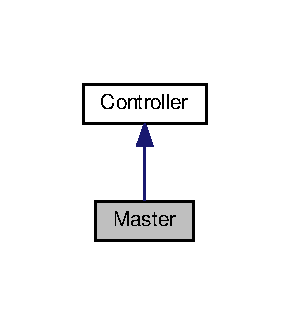
\includegraphics[width=139pt]{classMaster__inherit__graph}
\end{center}
\end{figure}


Collaboration diagram for Master\+:\nopagebreak
\begin{figure}[H]
\begin{center}
\leavevmode
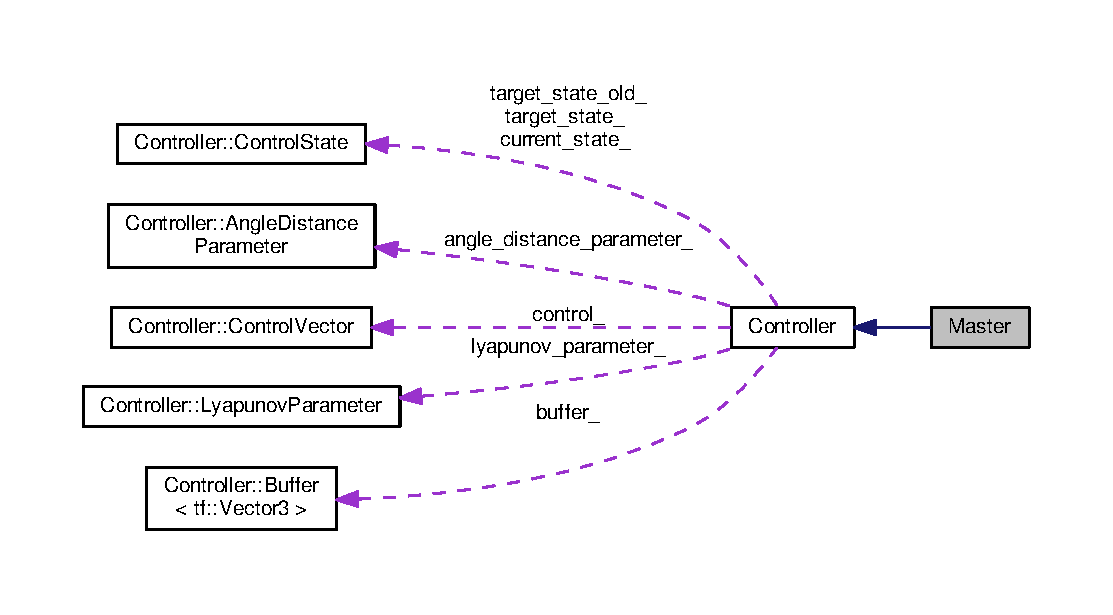
\includegraphics[width=350pt]{classMaster__coll__graph}
\end{center}
\end{figure}
\subsection*{Public Member Functions}
\begin{DoxyCompactItemize}
\item 
\hyperlink{classMaster_ab52840de45f9ce7022c9cf58cfb49398}{Master} (ros\+::\+Node\+Handle \&\hyperlink{classController_a24e3d3c2536f6ed29018bad1fd53dae2}{nh})
\begin{DoxyCompactList}\small\item\em Construct a new \hyperlink{classMaster}{Master} object. \end{DoxyCompactList}\end{DoxyCompactItemize}
\subsection*{Additional Inherited Members}


\subsection{Detailed Description}
Class that implements a master robot for multi robot formation control. 

\subsection{Constructor \& Destructor Documentation}
\index{Master@{Master}!Master@{Master}}
\index{Master@{Master}!Master@{Master}}
\subsubsection[{\texorpdfstring{Master(ros\+::\+Node\+Handle \&nh)}{Master(ros::NodeHandle &nh)}}]{\setlength{\rightskip}{0pt plus 5cm}Master\+::\+Master (
\begin{DoxyParamCaption}
\item[{ros\+::\+Node\+Handle \&}]{nh}
\end{DoxyParamCaption}
)}\hypertarget{classMaster_ab52840de45f9ce7022c9cf58cfb49398}{}\label{classMaster_ab52840de45f9ce7022c9cf58cfb49398}


Construct a new \hyperlink{classMaster}{Master} object. 


\begin{DoxyParams}{Parameters}
{\em nh} & Nodehandle \\
\hline
\end{DoxyParams}


The documentation for this class was generated from the following files\+:\begin{DoxyCompactItemize}
\item 
controller/include/controller/master.\+h\item 
controller/src/master.\+cpp\end{DoxyCompactItemize}

\hypertarget{classOdometryPredictor}{}\section{Odometry\+Predictor Class Reference}
\label{classOdometryPredictor}\index{Odometry\+Predictor@{Odometry\+Predictor}}
\subsection*{Public Member Functions}
\begin{DoxyCompactItemize}
\item 
{\bfseries Odometry\+Predictor} (ros\+::\+Node\+Handle \&nh)\hypertarget{classOdometryPredictor_a9b4cc16ef852f876d3628213e341d263}{}\label{classOdometryPredictor_a9b4cc16ef852f876d3628213e341d263}

\item 
{\bfseries Odometry\+Predictor} (ros\+::\+Node\+Handle \&nh, std\+::string topic\+\_\+name, tf\+::\+Transform initial\+\_\+trafo)\hypertarget{classOdometryPredictor_a18c088e85a802c82732fdc0f8dcbb961}{}\label{classOdometryPredictor_a18c088e85a802c82732fdc0f8dcbb961}

\item 
tf\+::\+Pose {\bfseries get\+Pose} ()\hypertarget{classOdometryPredictor_ac7c175fe97fec3d08c95be541c6551c9}{}\label{classOdometryPredictor_ac7c175fe97fec3d08c95be541c6551c9}

\end{DoxyCompactItemize}
\subsection*{Private Member Functions}
\begin{DoxyCompactItemize}
\item 
void {\bfseries callback\+Odometry} (const nav\+\_\+msgs\+::\+Odometry\+Const\+Ptr msg)\hypertarget{classOdometryPredictor_abfa0a69c2ba018d53e7976853366b833}{}\label{classOdometryPredictor_abfa0a69c2ba018d53e7976853366b833}

\end{DoxyCompactItemize}
\subsection*{Private Attributes}
\begin{DoxyCompactItemize}
\item 
ros\+::\+Node\+Handle {\bfseries nh\+\_\+}\hypertarget{classOdometryPredictor_a7f30f2dc41e540c0e22544ae08d4a793}{}\label{classOdometryPredictor_a7f30f2dc41e540c0e22544ae08d4a793}

\item 
ros\+::\+Subscriber {\bfseries odom\+\_\+sub\+\_\+}\hypertarget{classOdometryPredictor_a90649d9a1d3bfa1ee6a5bd0fee0a329c}{}\label{classOdometryPredictor_a90649d9a1d3bfa1ee6a5bd0fee0a329c}

\item 
std\+::string {\bfseries topic\+\_\+name\+\_\+}\hypertarget{classOdometryPredictor_a222da0dc75ff986e0105520cbf1a85d0}{}\label{classOdometryPredictor_a222da0dc75ff986e0105520cbf1a85d0}

\item 
tf\+::\+Transform {\bfseries initial\+\_\+trafo\+\_\+}\hypertarget{classOdometryPredictor_ab2d3f0deca499511a9b446d864a7ff66}{}\label{classOdometryPredictor_ab2d3f0deca499511a9b446d864a7ff66}

\item 
tf\+::\+Pose {\bfseries pose\+\_\+}\hypertarget{classOdometryPredictor_aae2765bb63f00d48860a50ff9b692910}{}\label{classOdometryPredictor_aae2765bb63f00d48860a50ff9b692910}

\end{DoxyCompactItemize}


The documentation for this class was generated from the following files\+:\begin{DoxyCompactItemize}
\item 
formation/include/formation/odometry\+\_\+predictor.\+h\item 
formation/src/odometry\+\_\+predictor.\+cpp\end{DoxyCompactItemize}

\hypertarget{classPlanner}{}\section{Planner Class Reference}
\label{classPlanner}\index{Planner@{Planner}}


Inheritance diagram for Planner\+:\nopagebreak
\begin{figure}[H]
\begin{center}
\leavevmode
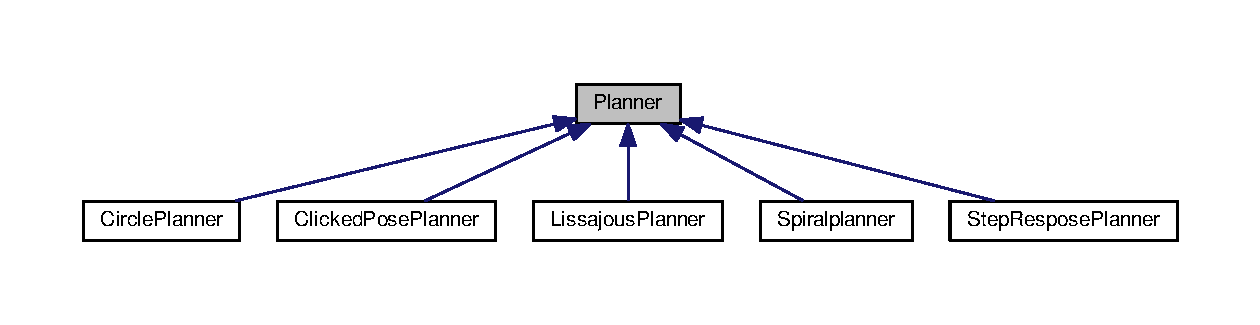
\includegraphics[width=264pt]{classPlanner__inherit__graph}
\end{center}
\end{figure}
\subsection*{Public Member Functions}
\begin{DoxyCompactItemize}
\item 
{\bfseries Planner} (ros\+::\+Node\+Handle \&\hyperlink{classPlanner_a9714d036f444a07ce90be8d135b9a40c}{nh})\hypertarget{classPlanner_a32475baddd401921adb1aab3ab842210}{}\label{classPlanner_a32475baddd401921adb1aab3ab842210}

\item 
void {\bfseries start} ()\hypertarget{classPlanner_a6c1c8d67d0cac41f738b413d1833c007}{}\label{classPlanner_a6c1c8d67d0cac41f738b413d1833c007}

\item 
void {\bfseries stop} ()\hypertarget{classPlanner_a3d0a3d404d39f59bfc21f275b0da408a}{}\label{classPlanner_a3d0a3d404d39f59bfc21f275b0da408a}

\item 
void {\bfseries pause} ()\hypertarget{classPlanner_a400f2aefad591e55a62e0fb13cb02521}{}\label{classPlanner_a400f2aefad591e55a62e0fb13cb02521}

\item 
void {\bfseries set\+\_\+start\+\_\+pose} (tf\+::\+Pose pose)\hypertarget{classPlanner_acaf55e0e250d6f3ba14bfcf3c4f06ffb}{}\label{classPlanner_acaf55e0e250d6f3ba14bfcf3c4f06ffb}

\item 
virtual void {\bfseries load} ()=0\hypertarget{classPlanner_af10d045ffe58c7d2149156567dc8b10a}{}\label{classPlanner_af10d045ffe58c7d2149156567dc8b10a}

\end{DoxyCompactItemize}
\subsection*{Protected Attributes}
\begin{DoxyCompactItemize}
\item 
int {\bfseries iterations\+\_\+counter}\hypertarget{classPlanner_a99b577203757a2466e8a3424c28d3449}{}\label{classPlanner_a99b577203757a2466e8a3424c28d3449}

\item 
ros\+::\+Node\+Handle \hyperlink{classPlanner_a9714d036f444a07ce90be8d135b9a40c}{nh}\hypertarget{classPlanner_a9714d036f444a07ce90be8d135b9a40c}{}\label{classPlanner_a9714d036f444a07ce90be8d135b9a40c}

\begin{DoxyCompactList}\small\item\em Counter for the iterations of periodic planner functions. \end{DoxyCompactList}\end{DoxyCompactItemize}
\subsection*{Private Member Functions}
\begin{DoxyCompactItemize}
\item 
void {\bfseries plan} (const ros\+::\+Timer\+Event \&events)\hypertarget{classPlanner_a6ccd3cb4a24886ddeff615e665f2fbbd}{}\label{classPlanner_a6ccd3cb4a24886ddeff615e665f2fbbd}

\item 
void {\bfseries publish} ()\hypertarget{classPlanner_aa8937e0a808cebc224393438941515e4}{}\label{classPlanner_aa8937e0a808cebc224393438941515e4}

\item 
tf\+::\+Transform \hyperlink{classPlanner_a311803ff0901b953c4ff9db7a3f5bb01}{get\+\_\+transform} (tf\+::\+Pose pose)
\item 
void \hyperlink{classPlanner_a0ce8028259452e2e17ed07bbb0c8463a}{transform\+\_\+values} (tf\+::\+Transform trafo)
\item 
bool \hyperlink{classPlanner_aef1abb6588a8fb7953183bc5f3479857}{srv\+\_\+start} (std\+\_\+srvs\+::\+Set\+Bool\+::\+Request \&req, std\+\_\+srvs\+::\+Set\+Bool\+::\+Response \&res)
\item 
bool \hyperlink{classPlanner_ac98453a1cd02d1d77055900f4fc4741f}{srv\+\_\+stop} (std\+\_\+srvs\+::\+Set\+Bool\+::\+Request \&req, std\+\_\+srvs\+::\+Set\+Bool\+::\+Response \&res)
\item 
virtual tf\+::\+Vector3 {\bfseries get\+\_\+position} (ros\+::\+Duration time)=0\hypertarget{classPlanner_ab388545a3fd2f37f70403d8484473a12}{}\label{classPlanner_ab388545a3fd2f37f70403d8484473a12}

\item 
virtual tf\+::\+Quaternion {\bfseries get\+\_\+orientation} (ros\+::\+Duration time)=0\hypertarget{classPlanner_a161fc00d031fd65914dae8f4b2edeffb}{}\label{classPlanner_a161fc00d031fd65914dae8f4b2edeffb}

\item 
virtual tf\+::\+Vector3 {\bfseries get\+\_\+velocity} (ros\+::\+Duration time)=0\hypertarget{classPlanner_a02af8b9ab29a19bd82c1cc35afcf2cc5}{}\label{classPlanner_a02af8b9ab29a19bd82c1cc35afcf2cc5}

\item 
virtual double {\bfseries get\+\_\+angular\+\_\+velocity} (ros\+::\+Duration time)=0\hypertarget{classPlanner_ab5c6ec661acf83b1f095ba404dc4c958}{}\label{classPlanner_ab5c6ec661acf83b1f095ba404dc4c958}

\item 
virtual void {\bfseries check\+\_\+period} (ros\+::\+Duration time)=0\hypertarget{classPlanner_a1bc7f9ca05b5de8aa4c9ccda126c2be2}{}\label{classPlanner_a1bc7f9ca05b5de8aa4c9ccda126c2be2}

\end{DoxyCompactItemize}
\subsection*{Private Attributes}
\begin{DoxyCompactItemize}
\item 
ros\+::\+Timer {\bfseries tim\+\_\+sampling}\hypertarget{classPlanner_a8dd2352bf15aef91d49337d95dfe6b04}{}\label{classPlanner_a8dd2352bf15aef91d49337d95dfe6b04}

\item 
ros\+::\+Publisher {\bfseries pub\+\_\+current\+\_\+odometry}\hypertarget{classPlanner_a1eea64fbf5b532bedd2f5a20eaedb4d8}{}\label{classPlanner_a1eea64fbf5b532bedd2f5a20eaedb4d8}

\item 
ros\+::\+Service\+Server {\bfseries set\+\_\+start\+\_\+service}\hypertarget{classPlanner_ad3cb4222b988ec69a5b89e1c67b119cd}{}\label{classPlanner_ad3cb4222b988ec69a5b89e1c67b119cd}

\item 
ros\+::\+Service\+Server {\bfseries set\+\_\+stop\+\_\+service}\hypertarget{classPlanner_a9211a5e71956ef94e1306adcabb2e51d}{}\label{classPlanner_a9211a5e71956ef94e1306adcabb2e51d}

\item 
bool {\bfseries is\+\_\+planning}\hypertarget{classPlanner_afcb5f703c4d2a54bb8c8f8360864b763}{}\label{classPlanner_afcb5f703c4d2a54bb8c8f8360864b763}

\item 
bool {\bfseries is\+\_\+paused}\hypertarget{classPlanner_a247ba912994c9035473b9ee037aac307}{}\label{classPlanner_a247ba912994c9035473b9ee037aac307}

\item 
int {\bfseries iterations}\hypertarget{classPlanner_a19220ea8cd70f4f3bfa3e35e1250ed00}{}\label{classPlanner_a19220ea8cd70f4f3bfa3e35e1250ed00}

\item 
std\+::string {\bfseries frame\+\_\+name}\hypertarget{classPlanner_a1578a9b87a63d6a806ab46a863ec55cb}{}\label{classPlanner_a1578a9b87a63d6a806ab46a863ec55cb}

\item 
ros\+::\+Duration {\bfseries paused}\hypertarget{classPlanner_a0e99faac21bce026cb9b0b576b734c71}{}\label{classPlanner_a0e99faac21bce026cb9b0b576b734c71}

\item 
ros\+::\+Time {\bfseries start\+\_\+time}\hypertarget{classPlanner_ade39963b5d3f74b75feed62ab669979e}{}\label{classPlanner_ade39963b5d3f74b75feed62ab669979e}

\item 
tf\+::\+Pose {\bfseries start\+\_\+pose}\hypertarget{classPlanner_af8043c3dfe8d863cec156f6b5abddd76}{}\label{classPlanner_af8043c3dfe8d863cec156f6b5abddd76}

\item 
tf\+::\+Vector3 {\bfseries planned\+\_\+vel}\hypertarget{classPlanner_a3d271654bd61b688e1db4f942722dd53}{}\label{classPlanner_a3d271654bd61b688e1db4f942722dd53}

\item 
tf\+::\+Vector3 {\bfseries vel}\hypertarget{classPlanner_aae4477f491ca6ba2e7f9ec2f0ca297c6}{}\label{classPlanner_aae4477f491ca6ba2e7f9ec2f0ca297c6}

\item 
tf\+::\+Vector3 {\bfseries pos}\hypertarget{classPlanner_a0f68f1ba4044c5a451e9352aed57ab9f}{}\label{classPlanner_a0f68f1ba4044c5a451e9352aed57ab9f}

\item 
tf\+::\+Quaternion {\bfseries orientation}\hypertarget{classPlanner_a3ce130c29c044931c6e8e7eeffd24c25}{}\label{classPlanner_a3ce130c29c044931c6e8e7eeffd24c25}

\item 
double {\bfseries ang\+\_\+vel}\hypertarget{classPlanner_a026af8deca2879d9f16b9eeddd003d88}{}\label{classPlanner_a026af8deca2879d9f16b9eeddd003d88}

\item 
tf\+::\+Transform {\bfseries start\+\_\+reference}\hypertarget{classPlanner_aae0304ebd1813766f1437b80d5195e90}{}\label{classPlanner_aae0304ebd1813766f1437b80d5195e90}

\end{DoxyCompactItemize}


\subsection{Member Function Documentation}
\index{Planner@{Planner}!get\+\_\+transform@{get\+\_\+transform}}
\index{get\+\_\+transform@{get\+\_\+transform}!Planner@{Planner}}
\subsubsection[{\texorpdfstring{get\+\_\+transform(tf\+::\+Pose pose)}{get_transform(tf::Pose pose)}}]{\setlength{\rightskip}{0pt plus 5cm}tf\+::\+Transform Planner\+::get\+\_\+transform (
\begin{DoxyParamCaption}
\item[{tf\+::\+Pose}]{pose}
\end{DoxyParamCaption}
)\hspace{0.3cm}{\ttfamily [private]}}\hypertarget{classPlanner_a311803ff0901b953c4ff9db7a3f5bb01}{}\label{classPlanner_a311803ff0901b953c4ff9db7a3f5bb01}
Gets the transformation form the given pose to the pose at timestamp zero 
\begin{DoxyParams}{Parameters}
{\em pose} & \+: Pose from wich the planner should start \\
\hline
\end{DoxyParams}
\index{Planner@{Planner}!srv\+\_\+start@{srv\+\_\+start}}
\index{srv\+\_\+start@{srv\+\_\+start}!Planner@{Planner}}
\subsubsection[{\texorpdfstring{srv\+\_\+start(std\+\_\+srvs\+::\+Set\+Bool\+::\+Request \&req, std\+\_\+srvs\+::\+Set\+Bool\+::\+Response \&res)}{srv_start(std_srvs::SetBool::Request &req, std_srvs::SetBool::Response &res)}}]{\setlength{\rightskip}{0pt plus 5cm}bool Planner\+::srv\+\_\+start (
\begin{DoxyParamCaption}
\item[{std\+\_\+srvs\+::\+Set\+Bool\+::\+Request \&}]{req, }
\item[{std\+\_\+srvs\+::\+Set\+Bool\+::\+Response \&}]{res}
\end{DoxyParamCaption}
)\hspace{0.3cm}{\ttfamily [private]}}\hypertarget{classPlanner_aef1abb6588a8fb7953183bc5f3479857}{}\label{classPlanner_aef1abb6588a8fb7953183bc5f3479857}
service procedure for satrting the planner 
\begin{DoxyParams}{Parameters}
{\em req} & \+: Reqest the service is getting \\
\hline
{\em res} & \+: Response the service is sending \\
\hline
\end{DoxyParams}
\index{Planner@{Planner}!srv\+\_\+stop@{srv\+\_\+stop}}
\index{srv\+\_\+stop@{srv\+\_\+stop}!Planner@{Planner}}
\subsubsection[{\texorpdfstring{srv\+\_\+stop(std\+\_\+srvs\+::\+Set\+Bool\+::\+Request \&req, std\+\_\+srvs\+::\+Set\+Bool\+::\+Response \&res)}{srv_stop(std_srvs::SetBool::Request &req, std_srvs::SetBool::Response &res)}}]{\setlength{\rightskip}{0pt plus 5cm}bool Planner\+::srv\+\_\+stop (
\begin{DoxyParamCaption}
\item[{std\+\_\+srvs\+::\+Set\+Bool\+::\+Request \&}]{req, }
\item[{std\+\_\+srvs\+::\+Set\+Bool\+::\+Response \&}]{res}
\end{DoxyParamCaption}
)\hspace{0.3cm}{\ttfamily [private]}}\hypertarget{classPlanner_ac98453a1cd02d1d77055900f4fc4741f}{}\label{classPlanner_ac98453a1cd02d1d77055900f4fc4741f}
service procedure for stopping the planner 
\begin{DoxyParams}{Parameters}
{\em req} & \+: Reqest the service is getting \\
\hline
{\em res} & \+: Response the service is sending \\
\hline
\end{DoxyParams}
\index{Planner@{Planner}!transform\+\_\+values@{transform\+\_\+values}}
\index{transform\+\_\+values@{transform\+\_\+values}!Planner@{Planner}}
\subsubsection[{\texorpdfstring{transform\+\_\+values(tf\+::\+Transform trafo)}{transform_values(tf::Transform trafo)}}]{\setlength{\rightskip}{0pt plus 5cm}void Planner\+::transform\+\_\+values (
\begin{DoxyParamCaption}
\item[{tf\+::\+Transform}]{trafo}
\end{DoxyParamCaption}
)\hspace{0.3cm}{\ttfamily [private]}}\hypertarget{classPlanner_a0ce8028259452e2e17ed07bbb0c8463a}{}\label{classPlanner_a0ce8028259452e2e17ed07bbb0c8463a}
Transforming all values that are not rotation or translation invariant 
\begin{DoxyParams}{Parameters}
{\em trafo} & \+: The Transformation applied to all values \\
\hline
\end{DoxyParams}


The documentation for this class was generated from the following files\+:\begin{DoxyCompactItemize}
\item 
simulation\+\_\+env/include/simulation\+\_\+env/planner.\+h\item 
simulation\+\_\+env/src/planner.\+cpp\end{DoxyCompactItemize}

\hypertarget{structFormation_1_1Robot}{}\section{Formation\+:\+:Robot Struct Reference}
\label{structFormation_1_1Robot}\index{Formation\+::\+Robot@{Formation\+::\+Robot}}


Holds a robot to handle with formation member stuff.  




{\ttfamily \#include $<$formation.\+h$>$}

\subsection*{Public Attributes}
\begin{DoxyCompactItemize}
\item 
tf\+::\+Pose \hyperlink{structFormation_1_1Robot_a63752bb5263e86b35e8f28f3c5948c88}{pose}\hypertarget{structFormation_1_1Robot_a63752bb5263e86b35e8f28f3c5948c88}{}\label{structFormation_1_1Robot_a63752bb5263e86b35e8f28f3c5948c88}

\begin{DoxyCompactList}\small\item\em Pose of the robot. \end{DoxyCompactList}\item 
\hyperlink{classFormation_a174a86b886bea3cb5d2c60526e73074d}{Neighbours} \hyperlink{structFormation_1_1Robot_a1a1dad64a86cf61f9c2633952a900b69}{neighbours}\hypertarget{structFormation_1_1Robot_a1a1dad64a86cf61f9c2633952a900b69}{}\label{structFormation_1_1Robot_a1a1dad64a86cf61f9c2633952a900b69}

\begin{DoxyCompactList}\small\item\em Neighbours of the robot. \end{DoxyCompactList}\item 
\hyperlink{classFormation_a57c79726ce19c016f8cb19ebe1b7f379}{Laser\+Pointer} \hyperlink{structFormation_1_1Robot_a01aa4b4c32c01bf74210d6e720815d33}{laser}\hypertarget{structFormation_1_1Robot_a01aa4b4c32c01bf74210d6e720815d33}{}\label{structFormation_1_1Robot_a01aa4b4c32c01bf74210d6e720815d33}

\begin{DoxyCompactList}\small\item\em \hyperlink{classLaserPredictor}{Laser\+Predictor} for this robot. \end{DoxyCompactList}\item 
Odom\+Pointer \hyperlink{structFormation_1_1Robot_a0b912dd3ce3e56cdc66261a981f7dc39}{odom}\hypertarget{structFormation_1_1Robot_a0b912dd3ce3e56cdc66261a981f7dc39}{}\label{structFormation_1_1Robot_a0b912dd3ce3e56cdc66261a981f7dc39}

\begin{DoxyCompactList}\small\item\em \hyperlink{classOdometryPredictor}{Odometry\+Predictor} for this robot. \end{DoxyCompactList}\item 
Odom\+Pointer \hyperlink{structFormation_1_1Robot_a770933c2c9760bc47c81a8d6579de317}{ekf}\hypertarget{structFormation_1_1Robot_a770933c2c9760bc47c81a8d6579de317}{}\label{structFormation_1_1Robot_a770933c2c9760bc47c81a8d6579de317}

\begin{DoxyCompactList}\small\item\em E\+KF Predictor for this robot. \end{DoxyCompactList}\end{DoxyCompactItemize}


\subsection{Detailed Description}
Holds a robot to handle with formation member stuff. 

The documentation for this struct was generated from the following file\+:\begin{DoxyCompactItemize}
\item 
formation/include/formation/formation.\+h\end{DoxyCompactItemize}

\hypertarget{structFormation_1_1RobotProperties}{}\section{Formation\+:\+:Robot\+Properties Struct Reference}
\label{structFormation_1_1RobotProperties}\index{Formation\+::\+Robot\+Properties@{Formation\+::\+Robot\+Properties}}


Defines Properties of a \hyperlink{structFormation_1_1Robot}{Robot}.  




{\ttfamily \#include $<$formation.\+h$>$}



Collaboration diagram for Formation\+:\+:Robot\+Properties\+:\nopagebreak
\begin{figure}[H]
\begin{center}
\leavevmode
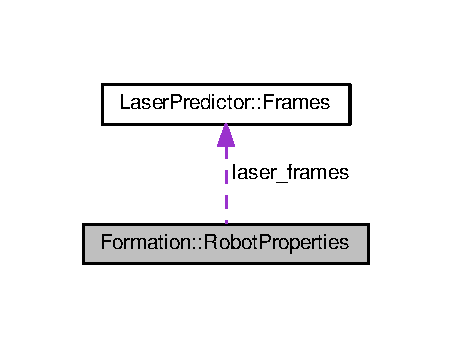
\includegraphics[width=217pt]{structFormation_1_1RobotProperties__coll__graph}
\end{center}
\end{figure}
\subsection*{Public Attributes}
\begin{DoxyCompactItemize}
\item 
std\+::string \hyperlink{structFormation_1_1RobotProperties_ade6ca62035362f280bab204b6a968541}{name}\hypertarget{structFormation_1_1RobotProperties_ade6ca62035362f280bab204b6a968541}{}\label{structFormation_1_1RobotProperties_ade6ca62035362f280bab204b6a968541}

\begin{DoxyCompactList}\small\item\em Name of the robot. \end{DoxyCompactList}\item 
tf\+::\+Pose \hyperlink{structFormation_1_1RobotProperties_a43b9b984481bb065f7170b09ce15e00b}{pose}\hypertarget{structFormation_1_1RobotProperties_a43b9b984481bb065f7170b09ce15e00b}{}\label{structFormation_1_1RobotProperties_a43b9b984481bb065f7170b09ce15e00b}

\begin{DoxyCompactList}\small\item\em Pose of the robot. \end{DoxyCompactList}\item 
\hyperlink{classFormation_a174a86b886bea3cb5d2c60526e73074d}{Formation\+::\+Neighbours} \hyperlink{structFormation_1_1RobotProperties_aed14aa20da03f0b2c37b5f891a8506ec}{neighbours}\hypertarget{structFormation_1_1RobotProperties_aed14aa20da03f0b2c37b5f891a8506ec}{}\label{structFormation_1_1RobotProperties_aed14aa20da03f0b2c37b5f891a8506ec}

\begin{DoxyCompactList}\small\item\em neighbours of the robot by name \end{DoxyCompactList}\item 
\hyperlink{structLaserPredictor_1_1Frames}{Laser\+Predictor\+::\+Frames} {\bfseries laser\+\_\+frames}\hypertarget{structFormation_1_1RobotProperties_ae8a53f87b542e2bf6bd05454b86dd012}{}\label{structFormation_1_1RobotProperties_ae8a53f87b542e2bf6bd05454b86dd012}

\item 
\hyperlink{classLaserPredictor_a3d60b85935a522f854a8f0a34bb7b3ca}{Laser\+Predictor\+::\+Topics} \hyperlink{structFormation_1_1RobotProperties_add5ddfcbb47487d1fb6c623a82bda89c}{laser\+\_\+topics}\hypertarget{structFormation_1_1RobotProperties_add5ddfcbb47487d1fb6c623a82bda89c}{}\label{structFormation_1_1RobotProperties_add5ddfcbb47487d1fb6c623a82bda89c}

\begin{DoxyCompactList}\small\item\em Topics the laserscanner messages are published at. \end{DoxyCompactList}\item 
std\+::string \hyperlink{structFormation_1_1RobotProperties_a23922628a06ebf33073ce00dd853b6ba}{odom\+\_\+topic}\hypertarget{structFormation_1_1RobotProperties_a23922628a06ebf33073ce00dd853b6ba}{}\label{structFormation_1_1RobotProperties_a23922628a06ebf33073ce00dd853b6ba}

\begin{DoxyCompactList}\small\item\em Name of the odometry topic. \end{DoxyCompactList}\item 
std\+::string \hyperlink{structFormation_1_1RobotProperties_a6b597cb09fe46f80f22853fcaf44bcae}{ekf\+\_\+topic}\hypertarget{structFormation_1_1RobotProperties_a6b597cb09fe46f80f22853fcaf44bcae}{}\label{structFormation_1_1RobotProperties_a6b597cb09fe46f80f22853fcaf44bcae}

\begin{DoxyCompactList}\small\item\em Name of the ekf topic. \end{DoxyCompactList}\end{DoxyCompactItemize}


\subsection{Detailed Description}
Defines Properties of a \hyperlink{structFormation_1_1Robot}{Robot}. 

The documentation for this struct was generated from the following file\+:\begin{DoxyCompactItemize}
\item 
formation/include/formation/formation.\+h\end{DoxyCompactItemize}

\hypertarget{classSlave}{}\section{Slave Class Reference}
\label{classSlave}\index{Slave@{Slave}}


Inheritance diagram for Slave\+:\nopagebreak
\begin{figure}[H]
\begin{center}
\leavevmode
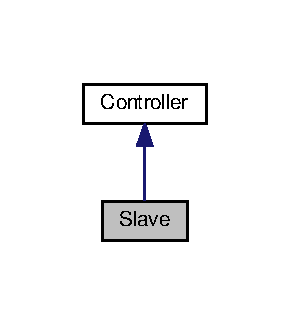
\includegraphics[width=139pt]{classSlave__inherit__graph}
\end{center}
\end{figure}


Collaboration diagram for Slave\+:\nopagebreak
\begin{figure}[H]
\begin{center}
\leavevmode
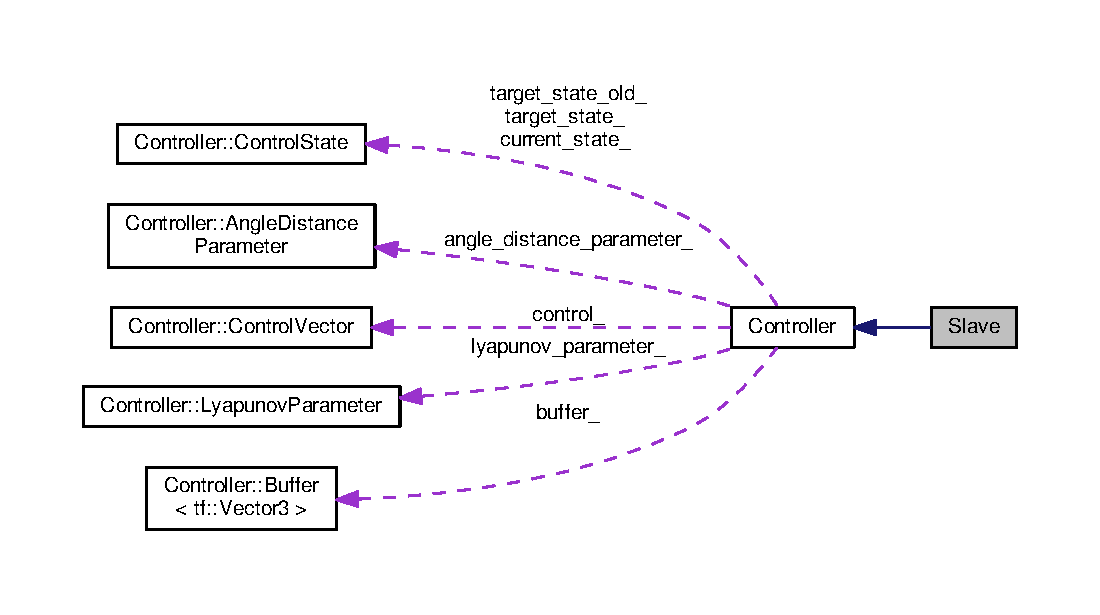
\includegraphics[width=223pt]{classSlave__coll__graph}
\end{center}
\end{figure}
\subsection*{Public Member Functions}
\begin{DoxyCompactItemize}
\item 
{\bfseries Slave} (ros\+::\+Node\+Handle \&\hyperlink{classController_a24e3d3c2536f6ed29018bad1fd53dae2}{nh})\hypertarget{classSlave_a855a824b462dd05eddaa8d53b27faea4}{}\label{classSlave_a855a824b462dd05eddaa8d53b27faea4}

\item 
void \hyperlink{classSlave_a9b5d1d499c7bd05d5260fbe5b8afbbb5}{scope} ()\hypertarget{classSlave_a9b5d1d499c7bd05d5260fbe5b8afbbb5}{}\label{classSlave_a9b5d1d499c7bd05d5260fbe5b8afbbb5}

\begin{DoxyCompactList}\small\item\em A Scope within the execute function. Repeating calculation in inheriting classes are implemented here. \end{DoxyCompactList}\end{DoxyCompactItemize}
\subsection*{Private Member Functions}
\begin{DoxyCompactItemize}
\item 
void \hyperlink{classSlave_a2a38a730d6ac93fcced035a7d764612d}{optimal\+\_\+control} ()
\item 
void \hyperlink{classSlave_a09394d0f823a06e04f6259ee490bc867}{target\+\_\+state\+\_\+callback} (geometry\+\_\+msgs\+::\+Pose\+Stamped msg)\hypertarget{classSlave_a09394d0f823a06e04f6259ee490bc867}{}\label{classSlave_a09394d0f823a06e04f6259ee490bc867}

\begin{DoxyCompactList}\small\item\em Callback for input target state message. Is executed everytima a target state input is incoming. Writes data to target\+\_\+pose state. \end{DoxyCompactList}\item 
void \hyperlink{classSlave_a2227f30ab058b623de7f6a940d079c90}{target\+\_\+velocities\+\_\+callback} (geometry\+\_\+msgs\+::\+Twist msg)\hypertarget{classSlave_a2227f30ab058b623de7f6a940d079c90}{}\label{classSlave_a2227f30ab058b623de7f6a940d079c90}

\begin{DoxyCompactList}\small\item\em Callback for input velocitiy message. Is executed everytime a velocitiy input is incoming. Writes data to input state. \end{DoxyCompactList}\item 
void \hyperlink{classSlave_a0d732637d1c0d06c214112a381ead6be}{target\+\_\+odometry\+\_\+callback} (nav\+\_\+msgs\+::\+Odometry msg)\hypertarget{classSlave_a0d732637d1c0d06c214112a381ead6be}{}\label{classSlave_a0d732637d1c0d06c214112a381ead6be}

\begin{DoxyCompactList}\small\item\em Callback for input target odometry message. Is executed everytima a target odometry input is incoming. Writes data to target\+\_\+pose state and target\+\_\+vel. \end{DoxyCompactList}\end{DoxyCompactItemize}
\subsection*{Private Attributes}
\begin{DoxyCompactItemize}
\item 
ros\+::\+Subscriber {\bfseries master\+\_\+odom}\hypertarget{classSlave_ae16b74032864ebb31211f992d37a73ab}{}\label{classSlave_ae16b74032864ebb31211f992d37a73ab}

\item 
tf\+::\+Pose {\bfseries master\+\_\+pose}\hypertarget{classSlave_ab6effa214fce2263784c296ecba8d3e0}{}\label{classSlave_ab6effa214fce2263784c296ecba8d3e0}

\end{DoxyCompactItemize}
\subsection*{Additional Inherited Members}


\subsection{Member Function Documentation}
\index{Slave@{Slave}!optimal\+\_\+control@{optimal\+\_\+control}}
\index{optimal\+\_\+control@{optimal\+\_\+control}!Slave@{Slave}}
\subsubsection[{\texorpdfstring{optimal\+\_\+control()}{optimal_control()}}]{\setlength{\rightskip}{0pt plus 5cm}void Slave\+::optimal\+\_\+control (
\begin{DoxyParamCaption}
{}
\end{DoxyParamCaption}
)\hspace{0.3cm}{\ttfamily [private]}}\hypertarget{classSlave_a2a38a730d6ac93fcced035a7d764612d}{}\label{classSlave_a2a38a730d6ac93fcced035a7d764612d}
This implements a least sqaures determination of control vector \mbox{[}v,omega\mbox{]} \mbox{[}control.\+v control.\+omega\mbox{]} from the given cartesian velocity state d/dt\mbox{[}x,y,phi\mbox{]} (cart\+\_\+vel) 

The documentation for this class was generated from the following files\+:\begin{DoxyCompactItemize}
\item 
controller/include/controller/slave.\+h\item 
controller/src/slave.\+cpp\end{DoxyCompactItemize}

\hypertarget{structSpiralplanner_1_1SpiralPlan}{}\section{Spiralplanner\+:\+:Spiral\+Plan Struct Reference}
\label{structSpiralplanner_1_1SpiralPlan}\index{Spiralplanner\+::\+Spiral\+Plan@{Spiralplanner\+::\+Spiral\+Plan}}
\subsection*{Public Attributes}
\begin{DoxyCompactItemize}
\item 
float {\bfseries r\+\_\+offset}\hypertarget{structSpiralplanner_1_1SpiralPlan_aa854c769a18405f2b69023063f4228a0}{}\label{structSpiralplanner_1_1SpiralPlan_aa854c769a18405f2b69023063f4228a0}

\item 
float {\bfseries r\+\_\+growth}\hypertarget{structSpiralplanner_1_1SpiralPlan_a64b2ae98f74cac59a2d35cc44f07f2d9}{}\label{structSpiralplanner_1_1SpiralPlan_a64b2ae98f74cac59a2d35cc44f07f2d9}

\item 
float {\bfseries omega}\hypertarget{structSpiralplanner_1_1SpiralPlan_a8cb0e1eca79013b8a84d4bf9162cb481}{}\label{structSpiralplanner_1_1SpiralPlan_a8cb0e1eca79013b8a84d4bf9162cb481}

\end{DoxyCompactItemize}


The documentation for this struct was generated from the following file\+:\begin{DoxyCompactItemize}
\item 
simulation\+\_\+env/include/simulation\+\_\+env/planner.\+h\end{DoxyCompactItemize}

\hypertarget{classSpiralplanner}{}\section{Spiralplanner Class Reference}
\label{classSpiralplanner}\index{Spiralplanner@{Spiralplanner}}


Inheritance diagram for Spiralplanner\+:\nopagebreak
\begin{figure}[H]
\begin{center}
\leavevmode
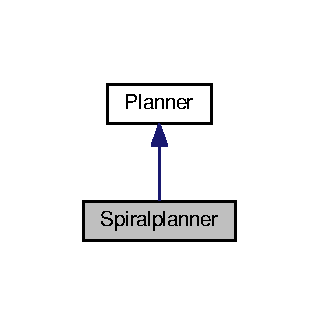
\includegraphics[width=153pt]{classSpiralplanner__inherit__graph}
\end{center}
\end{figure}


Collaboration diagram for Spiralplanner\+:\nopagebreak
\begin{figure}[H]
\begin{center}
\leavevmode
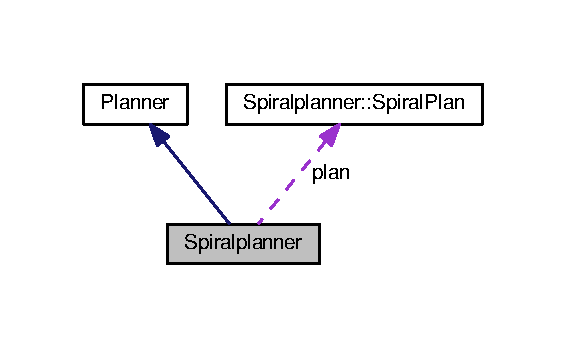
\includegraphics[width=272pt]{classSpiralplanner__coll__graph}
\end{center}
\end{figure}
\subsection*{Classes}
\begin{DoxyCompactItemize}
\item 
struct \hyperlink{structSpiralplanner_1_1SpiralPlan}{Spiral\+Plan}
\end{DoxyCompactItemize}
\subsection*{Public Member Functions}
\begin{DoxyCompactItemize}
\item 
{\bfseries Spiralplanner} (ros\+::\+Node\+Handle \&\hyperlink{classPlanner_a9714d036f444a07ce90be8d135b9a40c}{nh})\hypertarget{classSpiralplanner_af4fea271fc1dba2cde0d4e91e549ac00}{}\label{classSpiralplanner_af4fea271fc1dba2cde0d4e91e549ac00}

\item 
void {\bfseries set\+\_\+parameter} (double r\+\_\+offset, double r\+\_\+growth, double omega)\hypertarget{classSpiralplanner_a29bf0fc1aa4461c29fbe39e73f819b43}{}\label{classSpiralplanner_a29bf0fc1aa4461c29fbe39e73f819b43}

\item 
void {\bfseries load\+Child} ()\hypertarget{classSpiralplanner_a13b72cad3bd032c37f056303b7aeebf4}{}\label{classSpiralplanner_a13b72cad3bd032c37f056303b7aeebf4}

\end{DoxyCompactItemize}
\subsection*{Private Member Functions}
\begin{DoxyCompactItemize}
\item 
tf\+::\+Vector3 {\bfseries get\+\_\+position} (ros\+::\+Duration time)\hypertarget{classSpiralplanner_a5aacbbacdd271e9257bc6bb043d8c4e0}{}\label{classSpiralplanner_a5aacbbacdd271e9257bc6bb043d8c4e0}

\item 
tf\+::\+Quaternion {\bfseries get\+\_\+orientation} (ros\+::\+Duration time)\hypertarget{classSpiralplanner_ac6e8919f923ac0c4d888688a5d31503c}{}\label{classSpiralplanner_ac6e8919f923ac0c4d888688a5d31503c}

\item 
tf\+::\+Vector3 {\bfseries get\+\_\+velocity} (ros\+::\+Duration time)\hypertarget{classSpiralplanner_a4357a15b2fb9b585c17dee5a8662edfd}{}\label{classSpiralplanner_a4357a15b2fb9b585c17dee5a8662edfd}

\item 
double {\bfseries get\+\_\+angular\+\_\+velocity} (ros\+::\+Duration time)\hypertarget{classSpiralplanner_aea4f2405021302a3ceca29d485cd3f01}{}\label{classSpiralplanner_aea4f2405021302a3ceca29d485cd3f01}

\item 
tf\+::\+Vector3 {\bfseries get\+\_\+acceleration} (ros\+::\+Duration time)\hypertarget{classSpiralplanner_aac5f5d9c7b3180bbb8791b257445705c}{}\label{classSpiralplanner_aac5f5d9c7b3180bbb8791b257445705c}

\item 
void {\bfseries check\+\_\+period} (ros\+::\+Duration time)\hypertarget{classSpiralplanner_aa609defc35ad224a8f3bcb95d9cf8844}{}\label{classSpiralplanner_aa609defc35ad224a8f3bcb95d9cf8844}

\end{DoxyCompactItemize}
\subsection*{Private Attributes}
\begin{DoxyCompactItemize}
\item 
\hyperlink{structSpiralplanner_1_1SpiralPlan}{Spiral\+Plan} {\bfseries plan}\hypertarget{classSpiralplanner_a5aa839f0766271bdda12795126649ed6}{}\label{classSpiralplanner_a5aa839f0766271bdda12795126649ed6}

\end{DoxyCompactItemize}
\subsection*{Additional Inherited Members}


The documentation for this class was generated from the following files\+:\begin{DoxyCompactItemize}
\item 
simulation\+\_\+env/include/simulation\+\_\+env/planner.\+h\item 
simulation\+\_\+env/src/planner.\+cpp\end{DoxyCompactItemize}

\hypertarget{structStepResposePlanner_1_1StepPlan}{}\section{Step\+Respose\+Planner\+:\+:Step\+Plan Struct Reference}
\label{structStepResposePlanner_1_1StepPlan}\index{Step\+Respose\+Planner\+::\+Step\+Plan@{Step\+Respose\+Planner\+::\+Step\+Plan}}
\subsection*{Public Member Functions}
\begin{DoxyCompactItemize}
\item 
{\bfseries Step\+Plan} (std\+::vector$<$ float $>$ parameter)\hypertarget{structStepResposePlanner_1_1StepPlan_aede87fc069ba7e25ca148719ac28f68a}{}\label{structStepResposePlanner_1_1StepPlan_aede87fc069ba7e25ca148719ac28f68a}

\item 
{\bfseries Step\+Plan} (float delay, std\+::vector$<$ float $>$ parameter)\hypertarget{structStepResposePlanner_1_1StepPlan_ac5edeb9dfe1c66e8bf147198f70fb5ae}{}\label{structStepResposePlanner_1_1StepPlan_ac5edeb9dfe1c66e8bf147198f70fb5ae}

\end{DoxyCompactItemize}
\subsection*{Public Attributes}
\begin{DoxyCompactItemize}
\item 
std\+::vector$<$ float $>$ {\bfseries step\+\_\+sizes}\hypertarget{structStepResposePlanner_1_1StepPlan_afca5a2237ca3a290cb551f3189d578ef}{}\label{structStepResposePlanner_1_1StepPlan_afca5a2237ca3a290cb551f3189d578ef}

\item 
float {\bfseries delay\+\_\+time}\hypertarget{structStepResposePlanner_1_1StepPlan_ae532a987989c76a84f5e19b248c7cd9a}{}\label{structStepResposePlanner_1_1StepPlan_ae532a987989c76a84f5e19b248c7cd9a}

\end{DoxyCompactItemize}


The documentation for this struct was generated from the following file\+:\begin{DoxyCompactItemize}
\item 
simulation\+\_\+env/include/simulation\+\_\+env/planner.\+h\end{DoxyCompactItemize}

\hypertarget{classStepResposePlanner}{}\section{Step\+Respose\+Planner Class Reference}
\label{classStepResposePlanner}\index{Step\+Respose\+Planner@{Step\+Respose\+Planner}}


Inheritance diagram for Step\+Respose\+Planner\+:\nopagebreak
\begin{figure}[H]
\begin{center}
\leavevmode
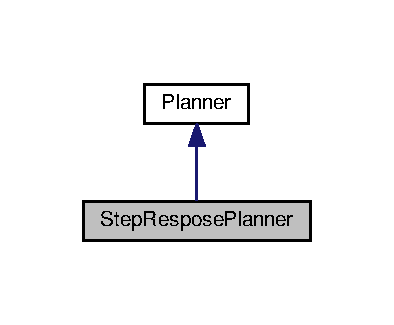
\includegraphics[width=189pt]{d5/d1c/classStepResposePlanner__inherit__graph}
\end{center}
\end{figure}


Collaboration diagram for Step\+Respose\+Planner\+:\nopagebreak
\begin{figure}[H]
\begin{center}
\leavevmode
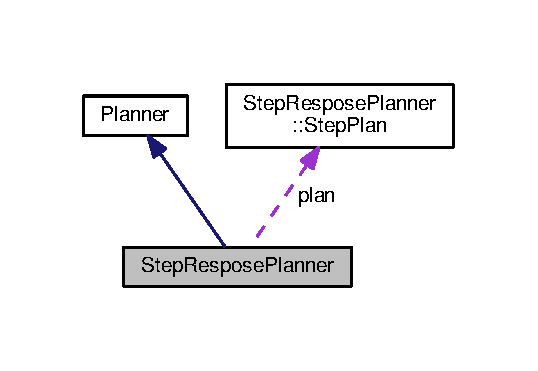
\includegraphics[width=258pt]{d6/de2/classStepResposePlanner__coll__graph}
\end{center}
\end{figure}
\subsection*{Classes}
\begin{DoxyCompactItemize}
\item 
struct \hyperlink{structStepResposePlanner_1_1StepPlan}{Step\+Plan}
\end{DoxyCompactItemize}
\subsection*{Public Member Functions}
\begin{DoxyCompactItemize}
\item 
{\bfseries Step\+Respose\+Planner} (ros\+::\+Node\+Handle \&\hyperlink{classPlanner_a9714d036f444a07ce90be8d135b9a40c}{nh})\hypertarget{classStepResposePlanner_afefbc3a96d82bcbce781e79730307bcb}{}\label{classStepResposePlanner_afefbc3a96d82bcbce781e79730307bcb}

\item 
void {\bfseries load\+Child} ()\hypertarget{classStepResposePlanner_a2fe2221f82b19b10cf4842caedcf3c3a}{}\label{classStepResposePlanner_a2fe2221f82b19b10cf4842caedcf3c3a}

\end{DoxyCompactItemize}
\subsection*{Private Member Functions}
\begin{DoxyCompactItemize}
\item 
tf\+::\+Vector3 {\bfseries get\+\_\+position} (ros\+::\+Duration time)\hypertarget{classStepResposePlanner_a5bdbf4b5df7c662d8b9bf0c79c9226b2}{}\label{classStepResposePlanner_a5bdbf4b5df7c662d8b9bf0c79c9226b2}

\item 
tf\+::\+Quaternion {\bfseries get\+\_\+orientation} (ros\+::\+Duration time)\hypertarget{classStepResposePlanner_a93d42c102eb19c7eefb52591c2c74901}{}\label{classStepResposePlanner_a93d42c102eb19c7eefb52591c2c74901}

\item 
tf\+::\+Vector3 {\bfseries get\+\_\+velocity} (ros\+::\+Duration time)\hypertarget{classStepResposePlanner_a1045bc185b58ef79410ff1f007cbe6e9}{}\label{classStepResposePlanner_a1045bc185b58ef79410ff1f007cbe6e9}

\item 
double {\bfseries get\+\_\+angular\+\_\+velocity} (ros\+::\+Duration time)\hypertarget{classStepResposePlanner_ac608ace99798a07f710ddd7eece983f6}{}\label{classStepResposePlanner_ac608ace99798a07f710ddd7eece983f6}

\item 
tf\+::\+Vector3 {\bfseries get\+\_\+acceleration} (ros\+::\+Duration time)\hypertarget{classStepResposePlanner_a30a5fb556a1576f9f1bc5f8300147202}{}\label{classStepResposePlanner_a30a5fb556a1576f9f1bc5f8300147202}

\item 
void {\bfseries check\+\_\+period} (ros\+::\+Duration time)\hypertarget{classStepResposePlanner_afb46272417c25b3b4304412bf25bded2}{}\label{classStepResposePlanner_afb46272417c25b3b4304412bf25bded2}

\end{DoxyCompactItemize}
\subsection*{Private Attributes}
\begin{DoxyCompactItemize}
\item 
\hyperlink{structStepResposePlanner_1_1StepPlan}{Step\+Plan} {\bfseries plan}\hypertarget{classStepResposePlanner_ac3fb95c79f21607429d8b6bd39e46451}{}\label{classStepResposePlanner_ac3fb95c79f21607429d8b6bd39e46451}

\item 
tf\+::\+Vector3 {\bfseries pos\+\_\+old\+\_\+}\hypertarget{classStepResposePlanner_a071fe84deb0d5fef56137d954cc3b98c}{}\label{classStepResposePlanner_a071fe84deb0d5fef56137d954cc3b98c}

\item 
tf\+::\+Vector3 {\bfseries pos\+\_\+new\+\_\+}\hypertarget{classStepResposePlanner_a201263730eb30540bb8ebdfae2548fc2}{}\label{classStepResposePlanner_a201263730eb30540bb8ebdfae2548fc2}

\item 
tf\+::\+Quaternion {\bfseries ori\+\_\+old\+\_\+}\hypertarget{classStepResposePlanner_a2bf8a7e217249ea9f8ecfb31d13bde7d}{}\label{classStepResposePlanner_a2bf8a7e217249ea9f8ecfb31d13bde7d}

\item 
tf\+::\+Quaternion {\bfseries ori\+\_\+new\+\_\+}\hypertarget{classStepResposePlanner_a6d30759d611861e771bc30116bda63af}{}\label{classStepResposePlanner_a6d30759d611861e771bc30116bda63af}

\end{DoxyCompactItemize}
\subsection*{Additional Inherited Members}


The documentation for this class was generated from the following files\+:\begin{DoxyCompactItemize}
\item 
simulation\+\_\+env/include/simulation\+\_\+env/planner.\+h\item 
simulation\+\_\+env/src/planner.\+cpp\end{DoxyCompactItemize}

\hypertarget{structLaserPredictor_1_1Transforms}{}\section{Laser\+Predictor\+:\+:Transforms Struct Reference}
\label{structLaserPredictor_1_1Transforms}\index{Laser\+Predictor\+::\+Transforms@{Laser\+Predictor\+::\+Transforms}}


Holds all necessary transformations.  




{\ttfamily \#include $<$laser\+\_\+predictor.\+h$>$}

\subsection*{Public Attributes}
\begin{DoxyCompactItemize}
\item 
tf\+::\+Stamped\+Transform \hyperlink{structLaserPredictor_1_1Transforms_ac9dbf63ff6bdd04249b2430571b667d8}{front}\hypertarget{structLaserPredictor_1_1Transforms_ac9dbf63ff6bdd04249b2430571b667d8}{}\label{structLaserPredictor_1_1Transforms_ac9dbf63ff6bdd04249b2430571b667d8}

\begin{DoxyCompactList}\small\item\em Transformation from front link to base link. \end{DoxyCompactList}\item 
tf\+::\+Stamped\+Transform \hyperlink{structLaserPredictor_1_1Transforms_a06e94a39aa0a24421366af139cf82f8e}{back}\hypertarget{structLaserPredictor_1_1Transforms_a06e94a39aa0a24421366af139cf82f8e}{}\label{structLaserPredictor_1_1Transforms_a06e94a39aa0a24421366af139cf82f8e}

\begin{DoxyCompactList}\small\item\em Transformation from back link to base link. \end{DoxyCompactList}\end{DoxyCompactItemize}


\subsection{Detailed Description}
Holds all necessary transformations. 

The documentation for this struct was generated from the following file\+:\begin{DoxyCompactItemize}
\item 
formation/include/formation/laser\+\_\+predictor.\+h\end{DoxyCompactItemize}

%--- End generated contents ---

% Index
\backmatter
\newpage
\phantomsection
\clearemptydoublepage
\addcontentsline{toc}{chapter}{Index}
\printindex

\end{document}
